% Generated by GrindEQ Word-to-LaTeX 
\documentclass{article} % use \documentstyle for old LaTeX compilers

\usepackage[utf8]{inputenc} % 'cp1252'-Western, 'cp1251'-Cyrillic, etc.
\usepackage[english]{babel} % 'french', 'german', 'spanish', 'danish', etc.
\usepackage{amsmath}
\usepackage{amssymb}
\usepackage{txfonts}
\usepackage{mathdots}
\usepackage[classicReIm]{kpfonts}
\usepackage{graphicx}

% You can include more LaTeX packages here 


\begin{document}

%\selectlanguage{english} % remove comment delimiter ('%') and select language if required


\noindent \textbf{Elite Leading Mutation Backtracking Search Algorithm for High-Dimensional Medical Data Feature Selection }

\noindent Jian Wang${}^{a}$, Yi Chen${}^{a}$, Huilai Zou${}^{b*}$, Chenglang Lu${}^{b}$, Ali Asghar Heidari${}^{c}$, Lei Liu${}^{d}$, Huiling Chen${}^{a*}$, Guoxi Liang${}^{e*}$


\noindent \textit{${}^{a}$ Key Laboratory of Intelligent Informatics for Safety \& Emergency of Zhejiang Province, Wenzhou University, Wenzhou 325035, China}

\noindent \textit{jona.wzu@gmail.com, kenyoncy2016@gmail.com}mailto:\textit{, }chenhuiling.jlu@gmail.com\textit{\underbar{}}

\noindent \textit{${}^{b}$ College of modern information technology, Zhejiang Institute of Mechanical and Electrical Engineering, Hangzhou, Zhejiang 310051}

\noindent gameai@126.com\textit{, 6160212@qq.com}

\noindent \textit{${}^{c}$${}^{\ }$School of Surveying and Geospatial Engineering, College of Engineering, University of Tehran, Tehran, Iran}

\noindent aliasghar68@gmaill.com\textit{\underbar{}}

\textit{${}^{d\ }$College of Computer Science, Sichuan University, Chengdu, Sichuan 610065, China}

liulei.cx@gmail.com\textit{}

\noindent \textit{${}^{e}$ Department of Artificial Intelligence, Wenzhou Polytechnic, Wenzhou 325035, China}

\noindent \textit{guoxiliang2017@gmail.com}

\noindent \textit{}

\noindent \textbf{\textit{*Corresponding Author: }}\textit{Huilai Zou (gameai@126.com), Huiling Chen (}chenhuiling.jlu@gmail.com) and\textit{ Guoxi Liang (guoxiliang2017@gmail.com)}

\noindent 
\section{Abstract}

\noindent The Backtracking Search Algorithm (BSA), a population-based algorithm categorized under evolutionary computation, is renowned for its exploration capabilities and superior numerical optimization prowess, thanks to its unique historical memory, along with mutation and crossover operators. However, the intrinsic randomness of the original BSA hinders its ability to effectively balance exploration and exploitation, thereby limiting its local exploitation capabilities necessary for refining solution accuracy near optimal regions identified by elite individuals. This study aims to mitigate the randomness inherent in the original BSA and dynamically balance the trade-off between the exploration and exploitation phases. Mutation and crossover operators have been modified to better utilize elite individual information, enhancing solution accuracy. The performance of the proposed Improved Backtracking Search Algorithm (IBSA) was validated against the benchmark IEEE CEC 2017 functions, comparing it with 23 state-of-the-art algorithms, which include 12 classical meta-heuristic algorithms (MAs) and 11 advanced versions. The experimental results demonstrate that IBSA outperforms the original BSA in both convergence speed and solution accuracy. Furthermore, to authenticate IBSA's practical engineering applications, a binary version of IBSA (bIBSA) was developed using a v-shaped transformation function and applied to feature selection tasks in real-life engineering problems across 12 medical datasets encompassing various disease scenarios. These were compared against eight classical feature selection optimizers. Performance indicators such as average fitness value, number of selected features, average error rate, and time cost from comparative experiments underscore bIBSA's superior optimization ability within the binary problem domain. These results affirm the efficiency and robustness of the proposed elite leading mutation strategy integrated within the IBSA algorithm.



\noindent \textbf{Keywords: }Backtracking search algorithm; Elite leading mutation strategy; Evolution algorithms; Global optimization; Feature selection\textbf{}


\section{  Introduction}

Across the multifaceted landscape of computer science, a diverse array of challenges is characterized as NP-hard problems. These span decision-making [1, 2] as well as combinatorial optimization tasks [3, 4], all of which, to our best understanding, defy resolution within polynomial time. Such problems present significant obstacles due to their inherent complexity and their widespread occurrence across a multitude of disciplines [5, 6]. The expanding fields of data science [7] and machine learning [8] have markedly underscored the urgency for devising robust and efficient algorithms capable of surmounting these NP-hard conundrums.

In illustrating the prevalence of NP-hard challenges, consider the iconic Traveling Salesman Problem (TSP) [9]. As a salient example, the TSP permeates numerous computational areas, influencing sectors from manufacturing, such as circuit board drilling [10] and DNA sequencing [11], to the operations of daily logistical planning [12]. Decades of studious research have reinforced that addressing these problems remains a balancing act between systematic scientific approaches and the artistry of innovation.

Nevertheless, the struggle with NP-hard problems extends beyond conventional computational disciplines. Emerging fields, notably machine learning [13], data mining [14], and bioinformatics [15], grapple with the rapid surge in complexity that characterizes these issues. In these spheres, proficiently unravelling NP-hard problems becomes integral, especially for effective data analytics in the era dominated by the vastness of big data.

Building upon the escalating intricacy brought forth by big data in fields like machine learning, our research concentrates on a particular subset of NP-hard challenges inherent in global optimization and feature selection. Global optimization is the quest for an ultimate configuration that garners the best possible outcome [16]. This quest becomes even more intricate when coupled with feature selection, a critical process in developing machine learning models that entails selecting a group of significant features [17]. This process spawns a complex assortment of decisions, encapsulating the quintessential nature of NP-hard issues. Amidst the "curse of dimensionality" [18], the task of selecting the most pertinent features within high-dimensional data sets becomes paramount. Traditional approaches to feature selection typically involve two main components: the search mechanism to generate viable feature sets and the corresponding evaluation criterion for these sets. Presently, search mechanisms predominantly employ stochastic methods, which represent a divergence from exhaustive or sequential searching, due to the practical impossibility of reviewing every possible feature subset amidst an exponentially large number of possibilities [19].

Advancing from the stochastic mechanisms now prevalent in feature selection, we categorize these methods into three distinct types: filter-based, embedded, and wrapper-based approaches. Filter-based methods scrutinize features based on inherent characteristics, independent of any learning algorithm [20]. Embedded methods meld the feature selection process with the classifier training, yielding feature sets directly from the learning classifiers [21]. Contrastingly, wrapper-based methods appraise feature sets by assessing the performance of a classifier specifically trained on those sets. This classifier's performance becomes the metric for the suitability of the feature sets [22, 23]. Notably, wrapper methods take into account feature interdependencies by assessing bundled features, unlike filter approaches that evaluate features in isolation, thereby overlooking potential synergistic or antagonistic interactions. Consequently, this research is dedicated to the development of an advanced wrapper-based algorithm.

In the wake of recognizing wrapper-based methods' superior effectiveness and optimization capabilities, the pursuit of developing and refining these algorithms has intensified among researchers keen to meet the challenges of the 'big data era.' In machine learning models, wrapper algorithms typically employ meta-heuristic algorithms (MAs) acclaimed for their robust global optimization capabilities [24]. MAs traditionally fall into four categories, as illustrated in Fig. 1: \eqref{GrindEQ__1_} Biology-inspired, such as Ant Colony Optimization (ACO) [25], Particle Swarm Optimization (PSO) [26], Artificial Bee Colony (ABC) [27], and Slime Mould Algorithm (SMA) [28]; \eqref{GrindEQ__2_} Physics-inspired, including Simulated Annealing (SA) [29], Gravitational Search Algorithm (GSA) [30], Sine Cosine Algorithm (SCA) [31], and Equilibrium Optimizer (EO) [32]; \eqref{GrindEQ__3_} Evolutionary, like Genetic Algorithm (GA) [33], Differential Evolution (DE) [34], Evolution Programming (EP) [35], and Evolution Strategies [36]; and \eqref{GrindEQ__4_} Human behavior-inspired, such as Teaching Learning Based Optimization (TLBO) [37], Political Optimizer (PO) [38], Harmony Search Algorithm (HAS) [39], and Brain Storm Optimization (BSO) [40]. Among these, PSO is exceedingly popular for global optimization due to its swift convergence and minimal parameter tuning, proving invaluable in feature selection tasks [41]. Similarly, Simulated Annealing, which simulates the methodical cooling of materials to minimize structural faults, boasts a wide array of applications across various domains. Abdel-Basset et al. [42] enhanced this technique by integrating it with the Harris Hawk Algorithm (HHO) and applying it to feature selection, achieving improved classification accuracy and computational efficiency. The Genetic Algorithm, drawing on Darwinian evolutionary concepts, has also been prevalent in research. Dong et al. [43] examined how the granularity level can affect classification accuracy and the size of the feature subset in feature selection, leading to the proposition of a granularity-optimized genetic algorithm for this purpose. Furthermore, the pedagogically-inspired TLBO has achieved recognition, with Hosseini et al. [44] introducing a binary version augmented by a mutation operator, successfully applied to feature selection, yielding an optimal feature subset.

The scope of these MAs extends well beyond mere optimization, their deployment in feature selection is pivotal across a spectrum of applications, spanning from nuanced medical diagnostics to the complexities of image analysis [45], the sculpting of neural networks [46], and the deciphering of natural language processing [47]. The impetus behind adopting these sophisticated algorithms transcends the reduction of computational demands, it envisions enhancing model clarity and mitigating the perils of overfitting [48]. Illustratively, Reddy et al. [49] introduced an innovative Adaptive Genetic Algorithm with Fuzzy Logic (AGAFL), targeting the early detection of heart disease. Their model boasts superior performance over existing methodologies, attributed to its adeptness at pinpointing critical features and finely-tuning classification criteria utilizing UCI datasets.

Yet, the journey through the extensive search space of feature subsets is not without tribulations. While the promise is vast, the practical application of these MAs often grapples with an excessive dependence on computational resources, a critical sensitivity to parameter calibration, and issues of run-time efficiency that cannot be overlooked [50, 51]. Moreover, the field's progression beyond the well-trodden path of single-objective feature selection methodologies calls for an increasingly nuanced approach. The objective now is not simply to curtail feature numbers but to achieve a concurrent maximization of model accuracy---a delicate balancing act necessitating more intricate strategies [52].

In response to these multifaceted challenges, our paper is firmly directed at refining the innovative backtracking search algorithm---categorized under evolution-based approaches---that addresses global optimization. We endeavor to adapt this algorithm to a binary context, applying a v-shaped function specifically tailored for the task of feature selection. The performance and resilience of our proposed algorithm are meticulously scrutinized by contrasting it with a total of 23 prominent algorithms in CEC 2017 benchmark functions and 8 binary optimizers dedicated to feature selection tasks. The contributions articulated in this paper unfold as follows:

\begin{enumerate}
\item  We pioneer an elite leading mutation strategy built upon the foundational BSA algorithm, distinguishing the elite individual and leveraging elite information to enhance local exploitation and the accuracy of solutions.

\item  Innovative operators, inspired by the introduced vector $m$, are devised to augment the local exploitation capabilities of non-elite individuals.

\item  To navigate the trade-off between exploration and exploitation adeptly, a self-adaptive parameter $s$ is integrated, orchestrating the shift between global and local crossover operators.

\item  The efficacy of our proposed algorithm in global optimization, along with its binary adaptation for feature selection, is corroborated through extensive experimental evaluation.
\end{enumerate}

This paper is organized as follows: Section 2 presents an extensive literature review, highlighting significant research and emerging trends pertinent to enhancing the BSA for NP-hard problems. Section 3 introduces the motivation behind our research and provides detailed information about the proposed algorithm---including its binary version---and analyzes its computational complexity. Section 4 offers a rigorous quality analysis and global optimization performance validation of our proposed algorithm by comparison with 23 recently proposed MAs. Section 5 explores practical applications in real-life engineering problems, employing the binary version of our proposed algorithm for feature selection tasks and comparing its performance against eight classical binary optimizers. Finally, Section 6 draws conclusions from our findings and discusses potential future directions for this research.

\begin{figure}[htbp]
  \centering
  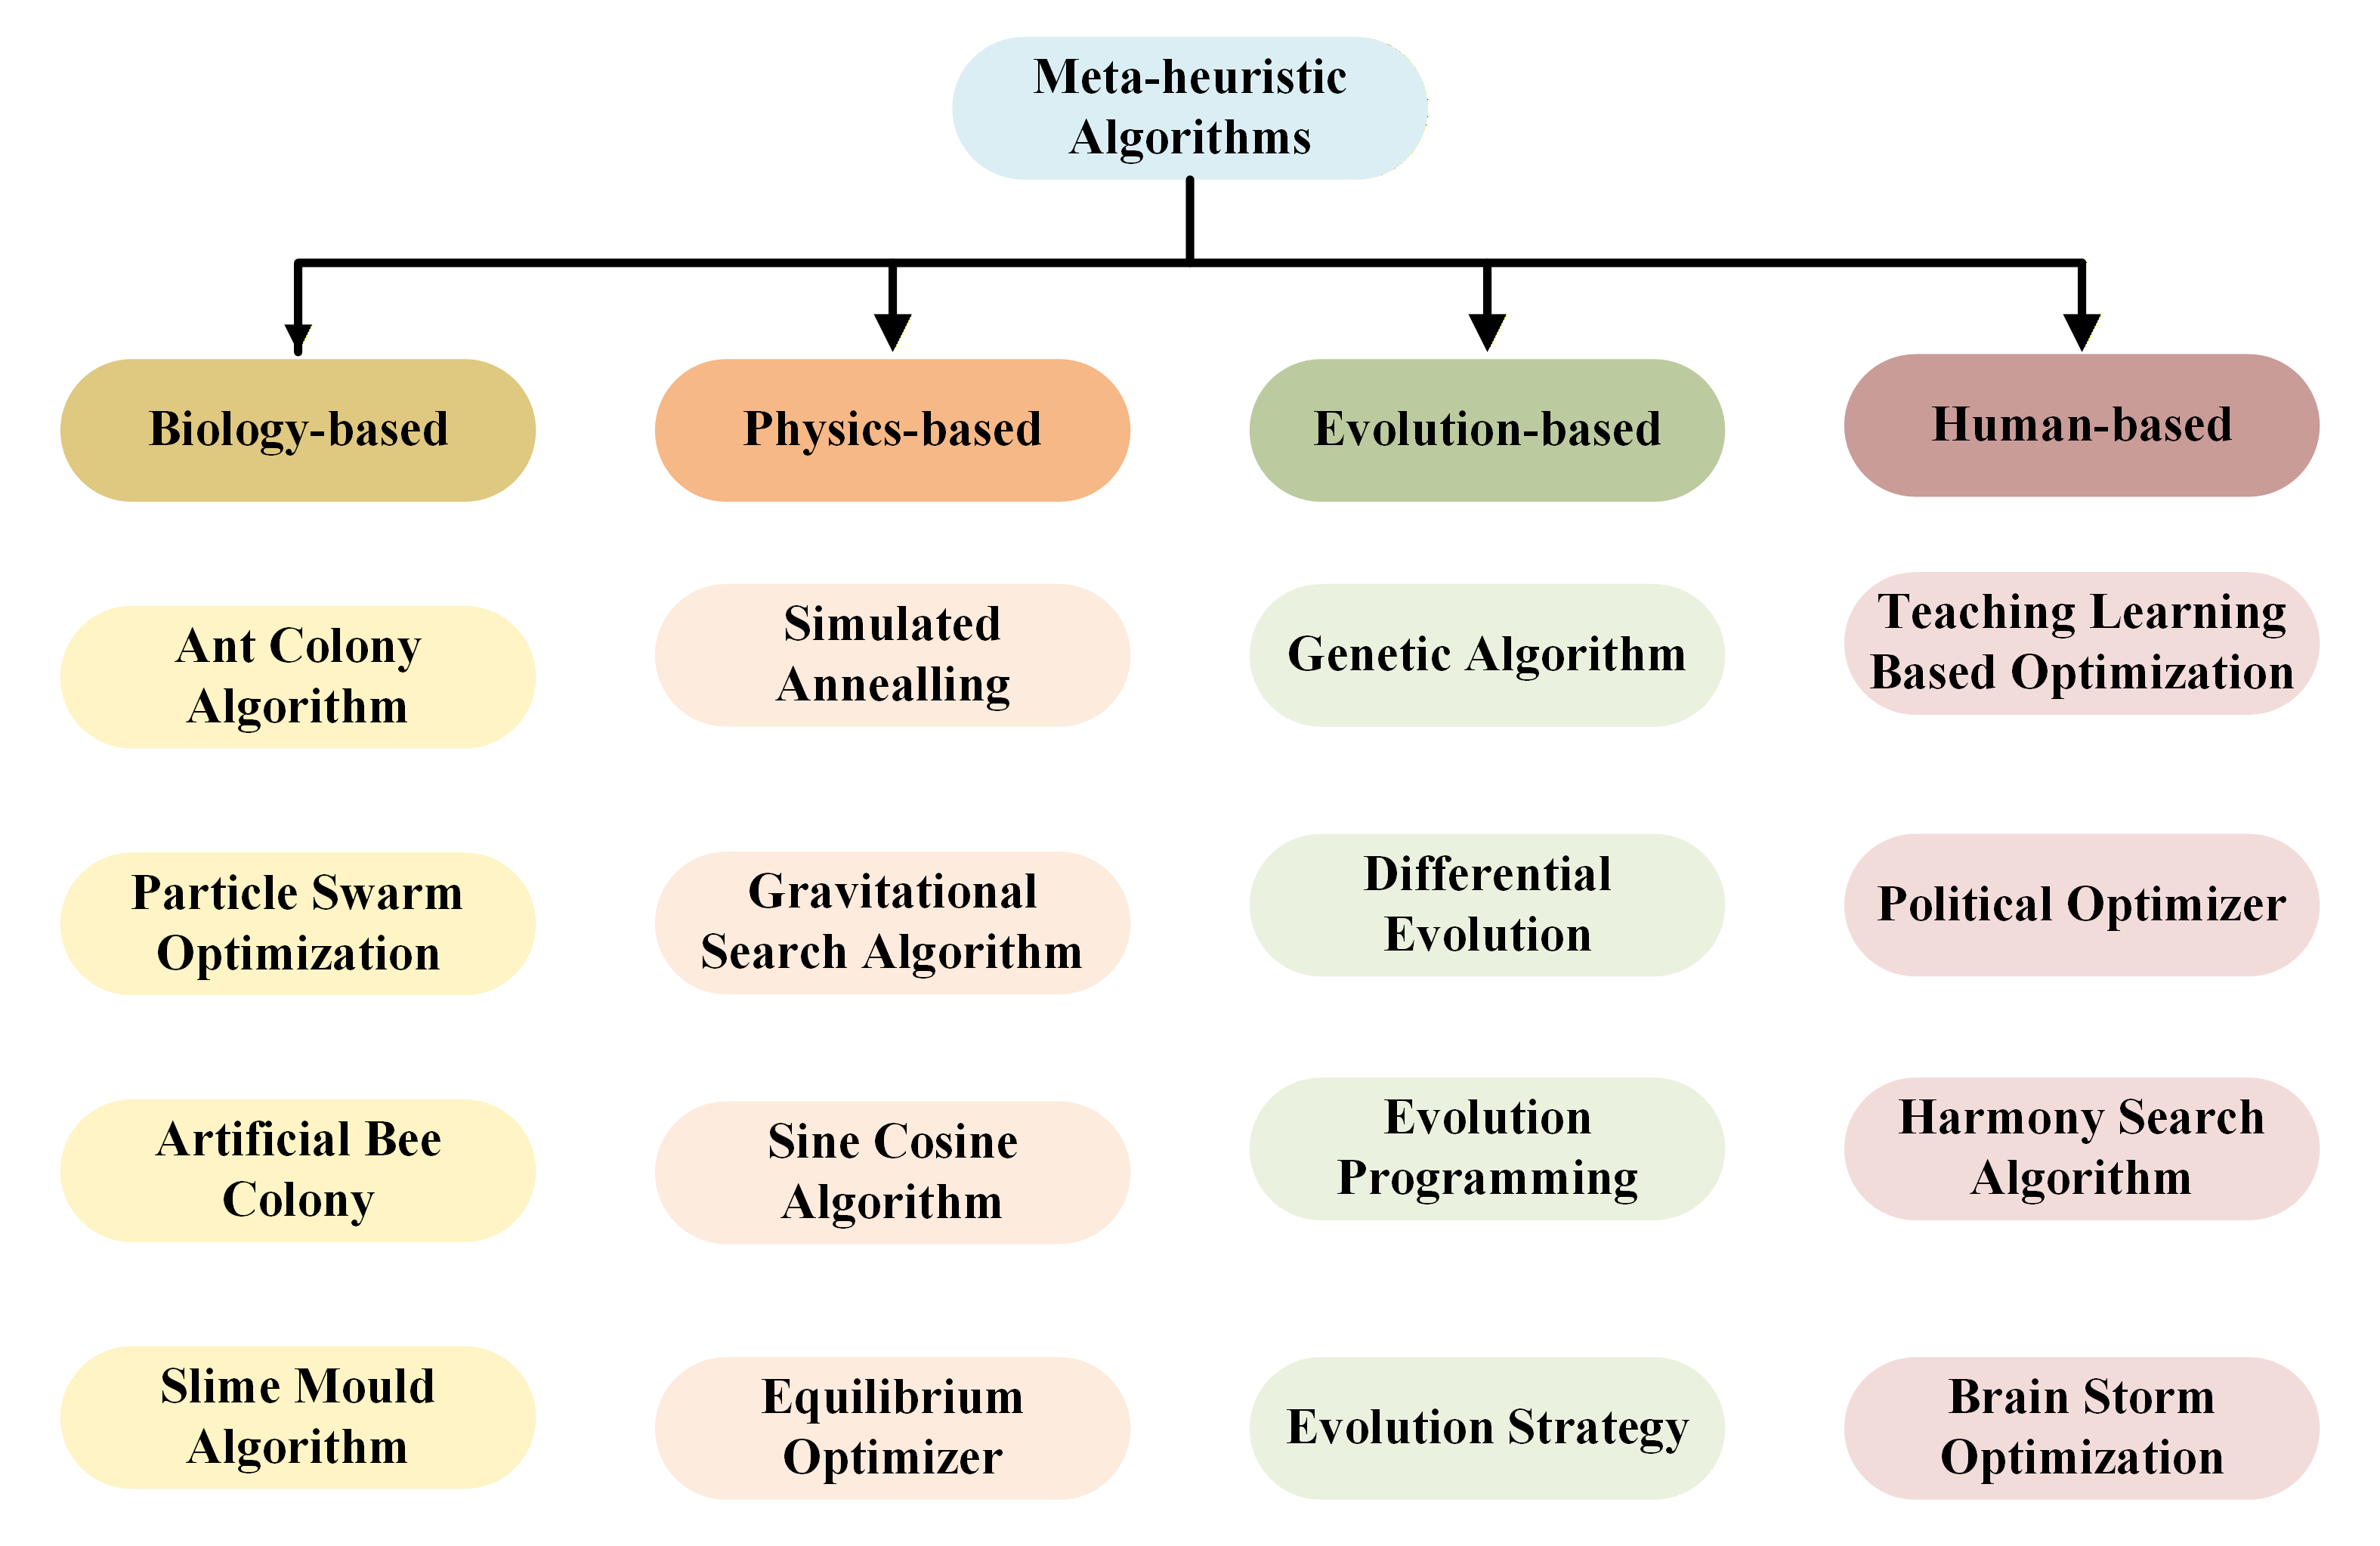
\includegraphics[width=\textwidth]{figures/fig1_classification_of_MAs.png}
  \caption{The four types of MAs.}
  \label{fig:classification_of_MAs}
\end{figure}


\section{ Literature review}

Introduced by Civicioglu in 2013, the BSA [53] has garnered attention for its uncomplicated yet effective architecture, particularly famed for its distinct memory strategies, which set it apart from Differential Evolution (DE) [34] and its acclaimed successors---JDE [54], JADE [55], and SADE [56]. The BSA's robust global search capability, stemming from its tolerance to variations in the parameter $F$, offers adaptability across diverse problems---users have the latitude to tune $F$ in alignment with the specific challenge at hand.

In its essence, BSA employs a single operator to engender a trial population, standing as the sole mechanism for population renewal within the evolutionary process. This operator harnesses the power of the existing population, in tandem with a direct search matrix, to amplify diversity---an attribute cherishing ease of use and accounting for BSA's widespread application. Nevertheless, this simplicity also surfaces as a constraint, as the algorithm's exploratory prowess overshadows its exploitative efficiency, impeding its quest for precise solutions [57].

Building upon the initial exposition of BSA's attributes, current research trends can be categorized into three distinctive strands, each aimed at overcoming continuous optimization challenges. Firstly, modifications to the original BSA are being explored to enhance algorithmic performance. Secondly, hybridization attempts are underway, melding BSA with other MAs to amalgamate their strengths and mitigate inherent weaknesses. Lastly, BSA's performance is being augmented through the integration of efficacious mechanisms and strategies. A detailed summarization of these research endeavors is presented below.

Continuing the discourse on BSA's evolution, a noteworthy adaptation is Zhang et al.'s [58] BSARDVs---an enhancement that capitalizes on the reutilization of differential vectors, eliminating the need for a central control parameter. This innovation positions it as a method unburdened by fine-tuning, boasting both efficiency and user-friendliness. When put to the test across three photovoltaic (PV) models, the BSARDVs demonstrated superior performance, outstripping competing algorithms with fewer function evaluations. Despite these advancements, the BSARDVs model has its own Achilles' heel: an exclusive reliance on historical populations and past differential vectors in its search strategy, without drawing on current population insights. This could inadvertently heighten the risk of convergence on local optima, particularly when addressing intricate optimization challenges.

Building on the modifications to BSA, Nama et al. [59] introduced a variant they christened gQR-BSA. This methodology harnesses the power of quantum Gaussian mutations alongside quasi-reflection-based jumps, a combination poised to deepen search efficiency within optimization problems. gQR-BSA, by reconfiguring the coordinate structure ingrained in the original BSA, seeks to transcend the rigidities of pre-established frameworks, augmenting the thoroughness of search space exploration which could pave the way for a leap in problem-solving efficacy. Despite these promising advancements, gQR-BSA does not escape scrutiny. The very act of balancing exploration with exploitation continues to be a delicate tightrope walk. Furthermore, the method grapples with computational complexity, an obstacle intrinsically woven into its fabric. These aspects beckon careful consideration as we chart the algorithm's trajectory in optimization realms.

Tsai et al. [60] delve into enhancements of the BSA, bringing forth ten distinct mutation tactics, each subjected to a comparative performance analysis. Alongside this array of strategies, the study carves out new parameters that draw upon historical averages and peak positions. A unidimensional crossover approach is also woven into the framework, serving as a bulwark against premature convergence. Yet, this innovative method is not without its trade-offs---introducing additional parameters puts a damper on user-friendliness and encumbers its ability to be seamlessly generalized across a spectrum of intricate optimization challenges.

In an effort to overcome one of the original BSA's shortcomings---the inability to learn from optimal individuals---Zhao et al. [61] introduced a Hierarchical Knowledge Guided BSA (HKBSA). This innovative approach is inspired by the patterns observed in nature, where living beings return to fruitful hunting grounds at sporadic junctures, thus increasing their chances of success. HKBSA weaves together self-learning and elite-learning strategies into the individual generation sequence, significantly enriching the diversity of the algorithm's population and bolstering its proficiency in learning and adaptation.

Zaman [62] masterminded a synergy between PSO (Particle Swarm Optimization) and BSA algorithms to birth PSOBSA---a hybrid with the intent to marry PSO's swift convergence with BSA's potent global exploration capacity. Tweaks to the mutation and crossover operators of BSA were strategized, aimed at honing convergence precision while avoiding the pitfalls of local optima. The hybrid's prowess in global optimization was put to the test across a suite of benchmark problems, attesting to its effectiveness. Nonetheless, the composite nature of PSOBSA does come with heightened complexity when juxtaposed with either algorithm alone, and a more intricate parameter tuning ordeal as well as heightened parameter sensitivity appear to be par for the course.

Chen et al. [63] cast light on an advanced iteration of the BSA, known as the Adaptive BSA with Knowledge Learning (KLBSA), which was conceived to amplify the algorithm's overall efficacy. This variant introduces an adaptive control parameter that leverages both global and local swarm intelligence, delicately calibrating the algorithm's exploration and exploitation competences. In addition, a groundbreaking mutation strategy is unveiled, aiming to boost the optimization function. To further escalate proficiency, a multi-population tactic is adopted, ensuring a rigorous probe across diverse search regions while safeguarding the variety within the population. However, the addition of multiple new strategies and parameters to KLBSA inevitably ratchets up the algorithm's complexity and may infuse the computational process with significant expense.

In their quest to bridge the divide between theoretical exploration and practical application, Lu et al. [64] bring forth a Hybrid Multi-Objective Backtracking Search Algorithm (HMOBSA) targeting the Permutation Flow Shop Scheduling Problem (PFSP) with a special focus on energy efficiency. This innovation underscores the often-neglected setup and transportation times, heralding sustainable manufacturing practices. The efficacy of HMOBSA is corroborated through its application in an authentic case scenario from a manufacturing firm. Nonetheless, it's important to note that the algorithm's sophistication and computational demands escalate due to the implementation of a dual population strategy and a self-adaptive selection mechanism. These attributes, while raising the complexity, concurrently augment the diversity and efficiency of the algorithm.

Diving into the realm of BSA research reveals a bounty of applications and enhancements. Nevertheless, to our cognizance, there is a conspicuous absence of studies employing BSA or its variants in medical data feature selection tasks. Given the exponential growth in big data and technological advancements, the sheer volume and complexity of medical data present a formidable obstacle in the patient treatment process. Addressing this lacuna, our paper introduces an augmented BSA variant that refines the original algorithm through sophisticated mutation and crossover modifications. This new strategy, dubbed the elite leading mutation strategy, is designed to amplify the inherent randomness of the original BSA and bolster the local exploitation prowess, distinguishing elite individuals from the rest to home in on more precise solutions. The enhanced model's efficacy and resilience have been substantiated against both the IEEE CEC 2017 benchmark suite and the intricate, real-world engineering challenge of high dimensional medical data feature selection.


\section{ Proposed methods}


\paragraph{ motivation}

The steadfast constants or probability constants are pivotal elements ingrained within MAs, serving as the cornerstone for harmonizing the crucial balance between exploration and exploitation. These parameters are traditionally dialed in through empirical experimentation, a process that can be exceedingly labor-intensive [65]. Yet, it's not a one-size-fits-all scenario, these constants may necessitate alterations to adapt to varying circumstances, such as distinct engineering conundrums. For instance, in the SA algorithm, a multitude of components like the normalization constant, initial temperature, cooling factor, and iteration count all sway its performance. Similarly, the crossover and mutation rates are critical knobs in the DE, demanding meticulous calibration for optimal efficacy. Furthermore, the Cuckoo Search Algorithm (CSA) [66] hinges on a switch parameter initially pegged at 0.25 to regulate local and global random walks, although it has fewer parameters compared to other MAs, CSA's success is tightly intertwined with this singular setting, calling for adjustments tailored to the specific problem domain.

This shared trait among various MAs has captivated a growing number of researchers to forge methodical solutions over the past two decades. A myriad of parameter-tuning methods have emerged as a result. Nevertheless, these approaches are not without their pitfalls. The omnipresent snag of non-universality and the necessity for numerous iterations across a gamut of parameters for each problem instance dampen these tuning methods' appeal, curtailing their application's scope. It's this ubiquitous challenge---the stringent requirements for algorithm parameter tuning - that stands as a formidable hurdle for other population-based optimization algorithms as well.

The BSA is ingeniously engineered to navigate through a diverse spectrum of problem landscapes, resorting to strategic backtracking as necessary to zero in on prime solutions---a trait that singularly marks its territory in the domain of evolutionary algorithms. At the core of BSA, five cardinal facets operate in concert: initialization, Selection I, Mutation, Crossover, and Selection II. These components coalesce to facilitate the algorithm's quest in the solution exploration, showcasing BSA as an adept and potent tool adept for deciphering the complexities of various problem areas.

\begin{enumerate}
\item  \textbf{Initialization:} This stage serves the vital purpose of spawning the initial population that speckles the vast solution space. The genesis of the initial population is governed by Eq. \eqref{GrindEQ__1_}.
\end{enumerate}

\begin{tabular}{|p{0.5in}|p{3.0in}|p{0.4in}|} \hline 
 & $X_i,_j=U(low_j,\ up_j)$ & (1) \\ \hline 
\end{tabular}

Here, $X$ stands for the swarm of candidate solutions. The variable $i$ indexes the individual members of this swarm, numbering from 1 to $N$, where $N$ denotes the total count of search agents within the population. Meanwhile, $j$ represents individual dimensions of the particular problem, which range from 1 to $D$, with $D$ signifying the problem's total dimensions. The terms $low$ and $up$ define the lower and upper bounds for the variables, respectively.

\begin{enumerate}
\item  \textbf{Selection I: }Within the BSA framework lies the critical Selection I phase, which plays an instrumental role in setting up the historical population. This historical population is a repository of accumulated information amassed throughout the evolutionary journey, serving as the foundational dataset for crafting the trial population during the mutation stage. This repository, symbolized as $OldX$, is computed through Eq. \eqref{GrindEQ__2_} and subsequently refined using Eq. \eqref{GrindEQ__3_} and Eq. \eqref{GrindEQ__4_}.
\end{enumerate}

\begin{tabular}{|p{0.5in}|p{3.0in}|p{0.4in}|} \hline 
 & $OldX_i,_j=U(low_j,\ up_j)$ & (2) \\ \hline 
\end{tabular}

The historical figures $OldX$ undergo an update, which unfolds as follows:

\begin{tabular}{|p{0.5in}|p{3.0in}|p{0.4in}|} \hline 
 & $OldX=\ \left\{ \begin{array}{c}
X\ \ \ \ \ \ \ \ \ \ \ \ \ \ \ \ \ if\ a<b \\ 
OldX\ \ \ \ \ \ \ \ \ \ \ \ \ \ Otherwise \end{array}
\right.$ & (3) \\ \hline 
\end{tabular}

In this context, $a$ and $b$ are randomly spawned numbers within the bracket of 0 to 1. This randomization injects a much-needed degree of variability into the process.

\begin{tabular}{|p{0.5in}|p{3.0in}|p{0.4in}|} \hline 
 & $OldX=permuting\left(OldX\right)$ & (4) \\ \hline 
\end{tabular}

The term $permuting(\cdot )$ encapsulates the action of shuffling the positions of the search agents within the population in a random fashion. This permutation plays a crucial role in fueling diversity within the population while also staving off the premature convergence of the algorithm toward subpar solutions.

\begin{enumerate}
\item  \textbf{Mutation:} The mutation phase plays a pivotal role within the BSA algorithm, where it employs both the historical and the current populations to spearhead the creation of the $Mutant$ population. This newly formed $Mutant$ set acts as the progenitor for the trial population. The mathematical operation defining this mutation is encapsulated by Eq. \eqref{GrindEQ__5_}.
\end{enumerate}

\begin{tabular}{|p{0.5in}|p{2.9in}|p{0.6in}|} \hline 
 & $Mutant=X+F\mathrm{\times }\left(oldX-X\right)$ & (5) \\ \hline 
\end{tabular}

In this equation, $F$ stands as a crucial amplitude control factor that notably sways the stretching of the $Mutant$ population. It achieves this by modulating the director matrix, which springs from the interplay between the historical $(OldX)$ and current $(X)$ populations. The chosen value for $F$ is derived from the expression $3\ *\ rndn$, wherein $rndn$ aligns with a standard normal distribution.

\begin{enumerate}
\item  \textbf{Crossover:} Post the mutation, we arrive at the creation of the final trial population, a crucial moment where crossover mechanics come into play. This is where two distinct parts become relevant. To commence, we establish a binary integer matrix, known as the $map$, with dimensions $N\ *\ D$ that initially contains only zeros. This $map$ is poised for an upgrade---a choice between two evolutionary paths influenced by either Eq \eqref{GrindEQ__6_}, the global crossover, or Eq \eqref{GrindEQ__7_}, the local crossover. In global crossover, numerous decision variables are simultaneously altered, whereas in local crossover, modification is restricted to a solitary decision variable within each solution. These pathways are not fixed but are rather randomly selected during each cycle of population generation, determining the crossover method to be applied to the trial population borne out of the mutation phase. The overarching aim is to either revitalize multiple facets of the solution or fine-tune singular aspects for optimized results. Defined by Eq \eqref{GrindEQ__8_}, elements of the final trial population $T$ are meticulously selected from the $Mutant$ and current populations based on the $map$ generated earlier.
\end{enumerate}

\begin{tabular}{|p{0.3in}|p{3.2in}|p{0.4in}|} \hline 
 & $map_i,_{u\left(1:\left\lceil M\mathrm{\times }rand\mathrm{\times }D\right\rceil \right)}=1\mathrm{\mid }u=permuting\left(1,2,3,\dots ,\ D\right),\ rand\in \left(0,\ 1\right)$ & (6) \\ \hline 
 & $map_i,_{randi\left(D\right)}=1$ & (7) \\ \hline 
 & $T\mathrm{=}\left\{ \begin{array}{c}
Mutant_i,_j\mathrm{,\ \ }map_i,_j=1 \\ 
X_i,_j\mathrm{,\ \ \ \ \ \ \ \ \ \ \ \ \ \ \ \ }map_i,_j=0 \end{array}
\right.$ & (8) \\ \hline 
\end{tabular}

The notation $\mathrm{\textrm{┌}}\mathrm{\ }\mathrm{\textrm{┐}}$ signifies the ceiling function, which effectively rounds up any real numbers to the nearest integer. The variable $M$ denotes the mix rate, serving as a control parameter that affects the extent of crossover for each search agent's decision variables. The function $permuting(\cdot )$ shuffles the order of decision variables, injecting an element of randomness into the process and enhancing the algorithm's robustness.

\begin{enumerate}
\item  \textbf{Selection II}: At this juncture within the BSA algorithm, we reach the Selection II phase, which hinges on the principle of greedy selection. Here, a decisive evaluation occurs between each corresponding member of the current population and their final trial counterpart. The one showcasing superior performance, as per a metric of choice, is retained, thus shaping the forthcoming generation. The criterion for selection within this phase is encapsulated by Eq \eqref{GrindEQ__9_}.
\end{enumerate}

\begin{tabular}{|p{0.4in}|p{2.9in}|p{0.5in}|} \hline 
 & $X_i=\ \left\{ \begin{array}{c}
T_i\ \ \ \ \ \ \ \ \ \ \ \ \ \ f\left(T_i\right)<f\left(X_i\right) \\ 
X_i\ \ \ \ \ \ \ \ \ \ \ \ \ \ Otherwise \end{array}
\right.$ & (9) \\ \hline 
\end{tabular}

In this formula,$\ f(\textrm{·})$ denotes the objective function---a measure designed to assess the quality of an individual solution. The terms  $T_i$ and $X_i$ correspond to the respective individuals from the final trial and the current populations. The process ensures that only those individuals who offer improved outcomes, as determined by the objective function, will progress into the next population. This method of selection is critical for fostering continuous improvement within the population, steering it towards ever-more-optimal solutions.

 We can conclude from the five components of the BSA that it only has one extra control parameter in the process of optimization. It will make the parameter-tuning process be more easy to tackle, and there may have a way to make the BSA a parameter-free algorithm so as to widen the application of BSA. Moreover, the BSA can not well balance the trades-off between the exploration and exploitation since the crossover of the basic trail population are randomly selected from two of the mapping operator [63]. So, the trail population only gather the information of the historical population and current population, and the elite information is not so well used. As we all know, we maintain the population diversity to decrease the possibility of trapping into local optimal. The BSA population use the historical information and current information to explore the promising area of the solution space. However, the precision of the solution is somewhat lost if the elite individual does not have a specific local search enhanced ability [67]. Besides, the basic trail population $Mutant$ have a critical influence of updating the BSA population location, but the historical population that guided the search direction are randomly selected. From the above analysis we can conclude although the BSA is elaborate designed, but there still have room to improve it and so as to make it can be used to solve real life problem without parameter-tuning more efficient. Based on the analysis we have made, this research proposed an elite leading mutation strategy which not only change the historical population selection decision but also separate the two crossover mechanism so as to balance the trade-off of exploration and exploitation and craft the solution accuracy.

In summarizing the essence of the BSA's structure, it becomes apparent that this system is characterized by its minimalistic approach to control parameters during the optimization process. This streamlined design facilitates a simpler parameter-tuning experience, hinting at the potential evolution of BSA towards a parameter-free model, which could significantly broaden its applicability. However, despite its ingenuity, BSA does not inherently ensure an equilibrium between exploration and exploitation---a result of its reliance on the random selection of crossover processes from two mapping operators [63]. Consequently, the trial population mainly incorporates data from historical and current populations, neglecting the valuable insights of the elite.

Preserving diverse genetic variety within the population is a universally recognized tactic to stave off convergence to local optima. While BSA adeptly navigates towards promising regions of the solution space by utilizing historical and present information, it regrettably sacrifices solution precision when elite individuals lack enhanced local search capabilities [67]. Moreover, the basic trial population, dubbed $Mutant$, significantly impacts the evolution of the populace's location, yet the guidance furnished by the historical population is randomized.

From this analysis, we discern that despite the thoughtfully crafted BSA, there exists an opportunity for refinement to further potentiate its efficacy in solving practical problems with greater efficiency and without the necessity for parameter-tuning. In alignment with our critical examination, the present study introduces an elite leading mutation Strategy, designed to not only refine the historical population's selection process but also to discretely unravel the dual crossover mechanisms. And aim to judiciously balance the scales of exploration and exploitation and to finetune the acuity of the solution.


\paragraph{ The Elite Leading Mutation Strategy}

 In the progression of our exposition on refinement strategies, we now divert our attention to section 3.2 encapsulating the elite leading mutation strategy. The conventional BSA is recognized for its intricate crossover approach, surpassing several of its evolutionary counterparts. However, it lacks the propensity to consistently employ fitness-superior individuals for exploration, as previously deliberated [53]. Notably, the erratic nature of map selection during crossover, coupled with the unpredictability in choosing the historical population, cultivates an environment of uncertainty, which particularly hampers the algorithm's precision in high-dimensional problems.

 In an innovative twist, inspired by the Random Spare Reinforced Whale Optimization Algorithm [68], a self-regulating parameter $s$ is introduced to refine the distinction between the current population and the optimal solution. As the population converges on a local optimum---indicated by stagnation in the location of the best search agent---the parameter $s$ dynamically increases, reciprocally decrementing to its square root upon discovering a superior solution. This parameter plays a pivotal role in defining the parameter $p$ which gauges the suitable mechanism for updating the $Mutant$, directed by Eq. \eqref{GrindEQ__11_}. The balanced trade-off between exploration and exploitation is achieved through the responsiveness of $s$, as elucidated in Eq. \eqref{GrindEQ__10_}. Here's the mathematical expression to update $s$ and $p$:

\begin{tabular}{|p{0.4in}|p{2.9in}|p{0.5in}|} \hline 
 & $s=\ \left\{ \begin{array}{c}
sqrt(s)\ \ \ \ \ \ \ \ \ \ \ \ \ \ \ \ \ if\ elite\ updated \\ 
s+1\ \ \ \ \ \ \ \ \ \ \ \ \ \ \ \ \ \ \ \ Otherwise \end{array}
\right.$ & (10) \\ \hline 
 & $p\ =\frac{sqrt\left(\frac{t}{Max\_FEs}\right)}{1\ +\ exp\left(-s\right)}$ & (11) \\ \hline 
\end{tabular}

Moving forward, the historical population selection is intricately entwined with the information derived from the crossover process. When a global crossover strategy substantially modifies the mutation population, it is strategically beneficial to employ this extensive information to direct future search trajectories. In this scenario, the historical population is selected, fostering an enhanced understanding of the solution space and thus improving the probability of identifying the optimal solution. Eq. \eqref{GrindEQ__12_} outlines the formulation of $OldX$, with $flag$ being determined by Eq. \eqref{GrindEQ__13_}:

\begin{tabular}{|p{0.4in}|p{2.9in}|p{0.5in}|} \hline 
 & $OldX=\ X\ \ \ if\ flag==1$ & (12) \\ \hline 
 & $flag=\ \left\{ \begin{array}{c}
1\ \ \ \ \ \ \ \ \ \ \ \ \ \ \ \ \ \ \ if\ global\ crossover \\ 
0\ \ \ \ \ \ \ \ \ \ \ \ \ \ \ \ \ \ \ Otherwise \end{array}
\right.$ & (13) \\ \hline 
\end{tabular}

 Additionally, a vector $m$ is allocated to non-elite individuals within the population. The magnitude of $m$ oscillates between -1 and +1, tapering to null as the evolutionary process matures, as defined in Eq. \eqref{GrindEQ__14_}. This measure ensures that the mutation's scope is localized, diversifying as warranted by the evolving conditions and contributing to the BSA's capacity to deftly navigate the exploration-exploitation continuum.

\begin{tabular}{|p{0.3in}|p{3.4in}|p{0.3in}|} \hline 
 & $m_i=\ \left\{ \begin{array}{c}
1\ \ \ \ \ \ \ \ \ \ \ \ \ \ \ \ \ \ \ \ \ \ \ \ \ \ \ \ \ \ \ \ \ \ \ \ \ \ \ \ \ \ \ if\ rand>\left(\frac{t}{Max\_FEs}\right)\wedge 3 \\ 
unifrnd(-\frac{t}{Max\_FEs},\frac{t}{Max\_FEs})\ \ \ \ \ \ \ \ \ \ \ \ Otherwise \end{array}
\right.$ & (14) \\ \hline 
\end{tabular}

 This strategically nuanced vector $m$ not only bolsters the BSA's explorative prowess but also disentangles elite from average individuals, endowing the former with a superior capability to pinpoint more precise solutions. Nevertheless, despite the enhancement it brings to the utilization of elite information, it does come at the cost of increased algorithmic complexity. The $Mutant$ operator adapts in accordance with Eq. \eqref{GrindEQ__15_}, and the elite are consequently refreshed as outlined by Eq. \eqref{GrindEQ__16_}.

\begin{tabular}{|p{0.3in}|p{3.4in}|p{0.3in}|} \hline 
 & ${\mathrm{Mutant}}_{\mathrm{i}}=m_i*\left(X_i+F*map_i\ .*\left(OldX_i-X_i\right)\right)\ \ \ if\ i\sim =BestX\_idx$ & (15) \\ \hline 
 & ${\mathrm{Mutant}}_{\mathrm{i}}=BestX+F*\left(OldX_i-X_i\right)\ \ \ if\ i==BestX\_idx$ & (16) \\ \hline 
\end{tabular}

Here, the subscript $i$ denotes the $i$th element respective to each variable, with matrix notations indicating row vectors and scalar notations representing individual elements. The $F$ value is defined as thrice the random number $rndn$ ranging between 0 to 1. 

Lastly, the pseudo-code for the Elite Leading Mutation Strategy is presented in \textbf{Algorithm 1} to visually convey the implementation details.

\begin{tabular}{|p{3.9in}|} \hline 
\textbf{Algorithm }1 Pseudo-code of Elite Leading Mutation Strategy \\ \hline 
Initialize $BestX,\ map,\ s,\ \ flag$; \\ \hline 
\textbf{If} $BestX$ updated \\ \hline 
    U$p$date $s$ by Eq. \eqref{GrindEQ__10_}; \\ \hline 
\textbf{End If} \\ \hline 
\textbf{If} $flag$ updated \\ \hline 
    Update $OldX$ by Eq. \eqref{GrindEQ__12_}; \\ \hline 
\textbf{End} \\ \hline 
$OldX\ =\ permuting(OldX)$; \\ \hline 
Calculate $p$ by Eq. \eqref{GrindEQ__11_}; \\ \hline 
\textbf{If} p $\mathrm{>}$ rand \\ \hline 
    Update $flag$ by Eq. \eqref{GrindEQ__13_}; \\ \hline 
    Update \textit{m} by Eq. \eqref{GrindEQ__14_}; \\ \hline 
    \textbf{For} $i\ =\ 1:N$ \\ \hline 
        \textbf{If} $i\ \sim =\ \boldsymbol{BestX}\boldsymbol{\_}\boldsymbol{idx}$ \\ \hline 
            Update $map$ by Eq. \eqref{GrindEQ__6_}; \\ \hline 
            Update Mutant by Eq. \eqref{GrindEQ__15_}; \\ \hline 
        \textbf{Else} \\ \hline 
            Update $Mutant$ by Eq. \eqref{GrindEQ__16_}; \\ \hline 
        \textbf{End If} \\ \hline 
    \textbf{End} \textbf{For} \\ \hline 
    \textbf{Else} \\ \hline 
\textbf{        }Update flag by Eq. \eqref{GrindEQ__13_}; \\ \hline 
\textbf{        For }$i\ =\ 1:N$ \\ \hline 
            Update $map$ by Eq. \eqref{GrindEQ__7_}; \\ \hline 
            Update Mutant by Eq. \eqref{GrindEQ__5_} and Eq. \eqref{GrindEQ__8_}; \\ \hline 
        \textbf{End For} \\ \hline 
    \textbf{End If} \\ \hline 
    Boundary control for $Mutant$; \\ \hline 
\textbf{End If} \\ \hline 
\end{tabular}




\paragraph{ The Proposed IBSA}

In this section, we delve into the intricacies of the proposed IBSA, a refined version of the original BSA enhanced by integrating the elite leading mutation strategy. This advanced IBSA is tailored to mitigate the inherent randomness and uncertainties observed in the foundational BSA's framework.

Reflecting on Civicioglu's optimization approach for BSA, it becomes evident that the historical population $(OldX)$, utilized for crafting the direction matrix, is conventionally derived from a random selection within the evolutionary lineage. This distinctive method sets BSA apart as a dual-population algorithm and starkly contrasts it with the deterministic designs of PSO, Covariance Matrix Adaptation Evolution Strategy (CMAES) [69], ABC, DE, and their variants. However, the haphazard method of historical sampling has been a pronounced downside, blurring the line between global exploration and exploitation due to the lack of directed search strategies.

To address these shortcomings, this research eschews random population selection in favor of clear-cut decision-making processes, establishing more predictable and dynamic trade-offs between exploration and exploitation. Whenever a global crossover incites considerable changes within the mutation population, suggesting an enhanced understanding of the solution space, the freshly-minted population assumes the role of $OldX$. Additionally, the newly introduced parameter $s$ plays a pivotal role in ascertaining the likelihood of the population becoming ensnared in local optima; it oscillates accordingly with mutation strategy probabilities, shaped into a non-linear curve exhibiting a steeper gradient at lower $s$ values and stabilizing as $s$ surpasses a certain threshold. Global crossovers are favored when $s$ and consequently $p$ are lower, supported by the design of $p$, which employs a modified sigmoid function for a nonlinear mapping from $s$ to a range between 0 and 1---a thoughtful adjustment ensuring a balanced interplay of mutation operators. As the evolutionary cycle matures, the focus drifts towards local crossover, with the randomized $rand$ metric determining the potential switch back to a global crossover stance.

Furthermore, both global mutation and crossover methodologies have been fine-tuned to reinforce local exploitation capabilities and capitalize on elite information for precision results.

IBSA is operationalized through a structured process:

In summary, the IBSA framework consists of the following key steps:

\begin{enumerate}
\item  Initialization:

\item  Preparing variables $X$, $OldX$, $BestFitness$, $PreBestFitness$, $BestX$, $map$, $s$, and $flag$.

\item  Selection-I:

\item  Calculating $s$ by subjecting $BestFitness$ with $PreBestFitness$.

\item  Deciding on historical population guided by $flag$.

\item  Mutation and Crossover:

\item  Determining $p$ from $s$.

\item  Electing mutation strategy (global or local) informed by $rand$ comparison with $p$, influencing flag accordingly.

\item  Selection-II:

\item  Iteratively refining $X$ through fitness comparison of each individual and the trial population.

\item  Udating $BestX$ and $BestFitness$.
\end{enumerate}

This sequence repeats until cessation criteria are attained, embodying the algorithm's intent to seek out finely tuned solutions via enhanced exploitation, escape from local optima, and judicious use of elite agents within the population.

The IBSA aims to significantly enhance the BSA's local search and exploitation capabilities while fully leveraging the elite information for more precise outcomes during the optimization process. The introduction of parameters $p$, which are intricately adjusted based on parameter $s$, are specifically designed to help the BSA population avoid becoming trapped in local optima. The use of vector $m$ further improves the local exploitation ability within the algorithm.

The mutation operator, thanks to the vector $m$, undergoes key modifications to distinguish elite individuals from the rest of the population, allowing for more tailored use of elite agent information. This differentiation facilitates strategic operation for each group, strengthening the algorithm's overall effectiveness.

To illustrate these changes, IBSA's procedural intricacies are codified within pseudo-code, designated as \textbf{Algorithm 2}, while a comprehensive flowchart detailing the steps and decision points of the algorithm is presented in Fig. 2. These tools serve to provide a clear visual understanding of IBSA's operational framework and the enhancements it brings to the BSA.

\begin{tabular}{|p{3.9in}|} \hline 
\textbf{Algorithm }2 Pseudo-code of IBSA \\ \hline 
Input $N,\ D,\ Max\_FEs,\ Lb,\ Ub,\ ObjFun$;\textit{} \\ \hline 
Initialize $X,\ OldX,\ BestFitness,\ PreBestFitness,\ BestX,\ map,\ s,\ \ flag$; \\ \hline 
\textbf{While} $t\ <\ Max\_FEs$ \\ \hline 
    Calculate and sort fitness of $X$; \\ \hline 
    Update $BestFitness,\ PreBestFitness,\ BestX,\ BestX\_idx$; \\ \hline 
\textbf{    Carry out Elite Leading Mutation Strategy;} \\ \hline 
    Calculate fitness of $Mutant$; \\ \hline 
    Update $X$ by Eq. \eqref{GrindEQ__9_}; \\ \hline 
    $t\ =\ t\ +\ 1$; \\ \hline 
\textbf{End While} \\ \hline 
\textbf{Return} \textit{B}$estFitness,\ BestX$. \\ \hline 
\end{tabular}



\begin{figure}[htbp]
  \centering
  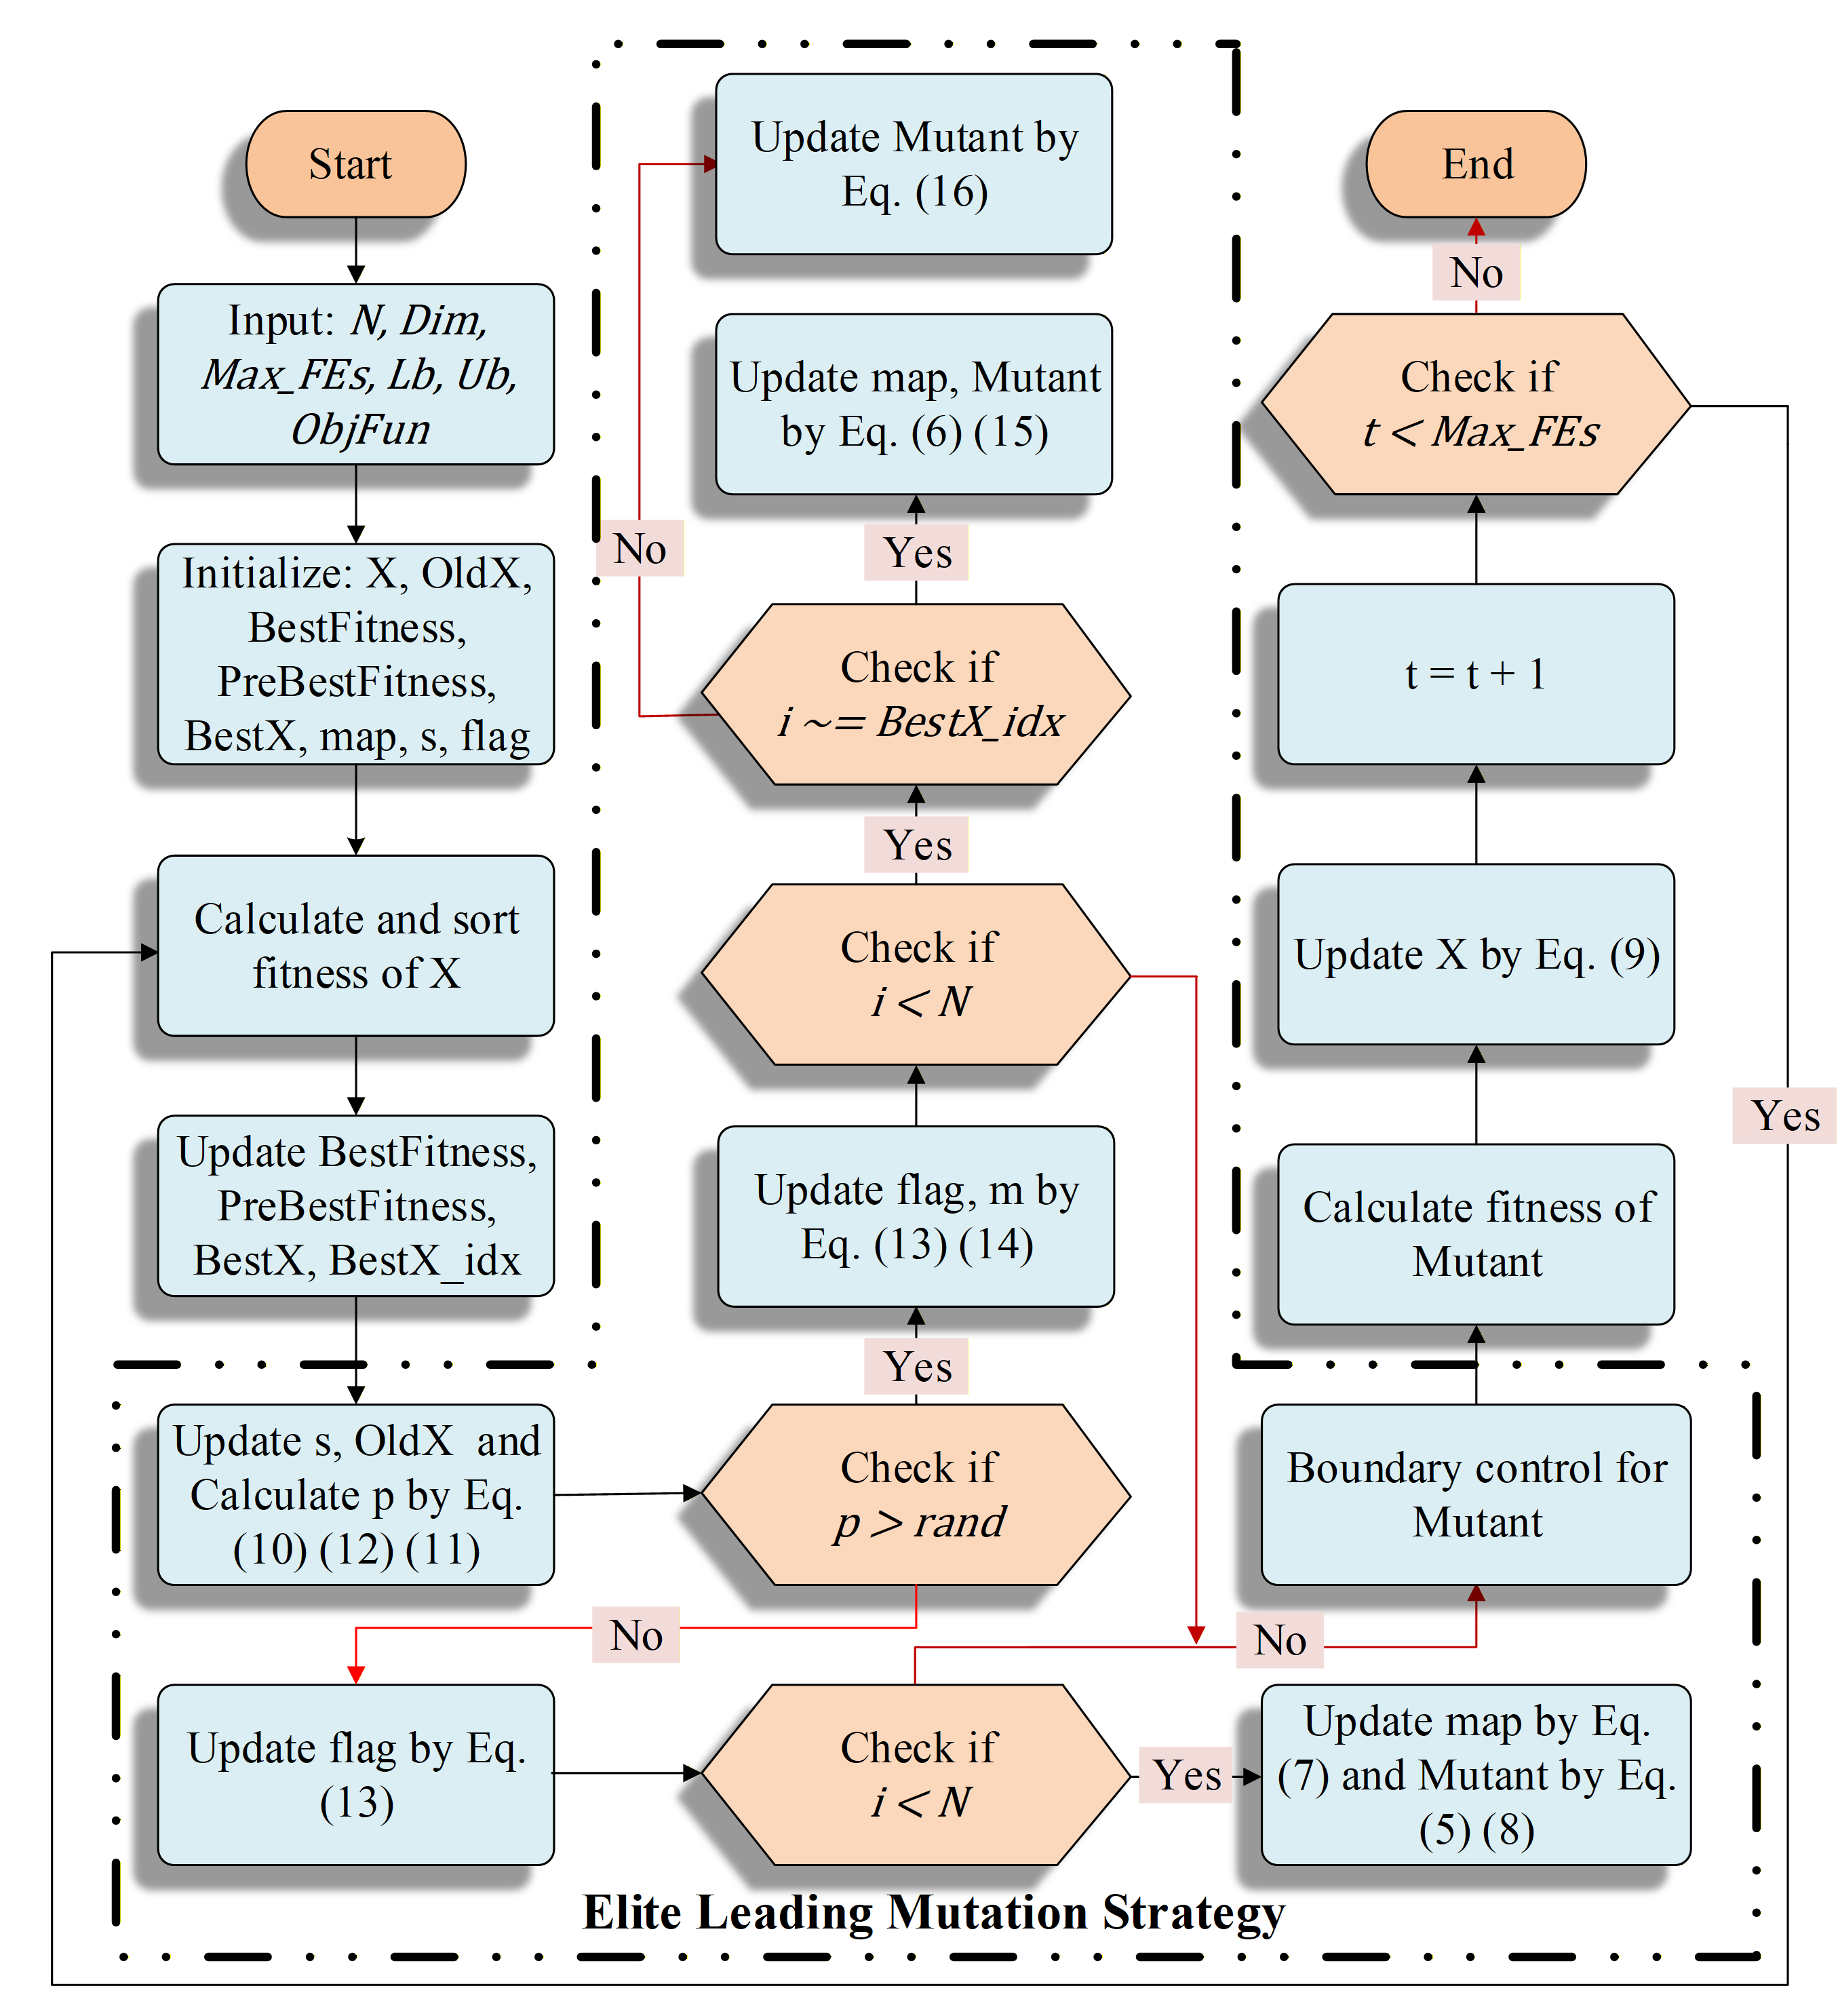
\includegraphics[width=\textwidth]{figures/fig2_flowchart_IBSA.png}
  \caption{Flowchart of IBSA.}
  \label{fig:flowchart_IBSA}
\end{figure}


\paragraph{ Binary IBSA for FS problem}

In this section, we turn our attention to the binary IBSA (bIBSA), ingeniously designed for binary discrete problem spaces, with a particular application to feature selection tasks in this study. The intricacies of bIBSA are geared towards effectively navigating the combinatorial challenges presented by feature subset selection, which, given $n$ features, results in potentially $2^n$ combinations.

To manage the complexity of evaluating such an extensive array of feature subsets, the bIBSA is teamed up with the KNN classifier [70] as an integral component of each iteration within the algorithm. A detailed diagram, Fig. 3, visualizes the overarching wrapper method process, highlighting its role in the decision-making pathway. The necessity for a discerning filter becomes clear here---without it, the evaluation phase would impose an impractical computational burden.

Leveraging the IBSA's robust capabilities in exploration and its advancements in exploitation, we incorporate a v-shaped transfer function [71] that succinctly transforms the algorithm into its binary counterpart bIBSA. This adaptation is crucial in narrowing down the subsets needing assessment by the classifier, hence conserving computational effort. Within the binary domain, the bIBSA exhibits a heightened level of straightforwardness relative to its continuous counterpart. This stems from the binary limitation of each feature dimension that oscillates strictly between 0 and 1, shaping a hypercubic search space wherein the algorithm's agents explore discrete corners by bit-by-bit shifts.

The forthcoming segment promises a comprehensive revelation of the IBSA-to-bIBSA transition, elucidating the decision logic that underpins these agents' searches. The fitness function, relying on the KNN classifier, serves as the evaluative compass for bIBSA, directing it towards an ideal balance of precision and succinctness in feature selection. The dual aims of maximizing accuracy while minimizing feature count are the hallmarks of this optimization pursuit.

The v-shaped transfer function is meticulously tailored to meet the needs of the Binary Improved Backtracking Search Algorithm, optimizing its performance for binary search spaces. Renowned for its distinctive characteristics, the function also sees wide application in fields such as signal processing and control systems. The transition of IBSA search agents' positions is governed by the rule defined in Eq. \eqref{GrindEQ__18_}.

A salient benefit of employing the v-shaped function in bIBSA is its gentle approach to binary decision-making. It does not rigidly impose binary values upon the decision variables, rather, it nudges them towards a binary state by incentivizing the flipping of a dimension's value if a more promising location is likely, according to Eq. \eqref{GrindEQ__17_}. Conversely, if no better prospects are detected, the algorithm permits the value to remain as is, leveraging the current position of the search agent to inform this decision.

This transitionary mechanism between continuous and binary domains conserves the core functional operators of the original IBSA. Thus, the bIBSA retains the essence of IBSA's operation, despite the shift in the problem domain. The operators' continuity ensures that the bIBSA upholds the pioneering characteristics of IBSA, while it embarks on the exploration within the binary hypercube.

\begin{tabular}{|p{0.4in}|p{2.9in}|p{0.5in}|} \hline 
 & $V\left(X^j_i\left(t\right)\right)=\left|\frac{2}{π}*\mathrm{atan}\mathrm{}(\frac{π}{2}*X^j_i\left(t\right))\right|$ & (17) \\ \hline 
 & $X^j_i\left(t+1\right)\mathrm{=}\left\{ \begin{array}{c}
1\mathrm{,\ \ }\ r\ \ge V\left(P^j_i\left(t\right)\right) \\ 
0\mathrm{,\ \ }\ r<V\left(P^j_i\left(t\right)\right) \end{array}
\right.$ & (18) \\ \hline 
\end{tabular}

Here, $X^j_i\left(t\right)$ represents the position of the $i$th search agent in the $j$th dimension at the $t$th iteration. The outcome of Eq. \eqref{GrindEQ__17_} remains a continuous value, which then, pursuant to Eq. \eqref{GrindEQ__18_}, is converted into a binary number if it exceeds the designated threshold.

The pursuit of optimizing features within a binary search space invariably presents itself as a multi-objective quest where the primary objectives are to minimize the number of selected features and simultaneously enhance classification accuracy to the greatest extent possible. This delicate balance underscores the essence of feature selection and is the driving force behind the refinement of solutions within bIBSA.

Each solution uncovered by bIBSA undergoes a rigorous evaluative process by a fitness function intrinsically linked to a KNN classifier. This fitness function plays an instrumental role in weighing the two critical aspects of feature selection---quantity and quality---the number of features and their collective predictive accuracy, respectively. The function, denoted by Eq. \eqref{GrindEQ__19_}, is integral to the assessment of each potential solution visited by the algorithm.

\begin{tabular}{|p{0.4in}|p{2.9in}|p{0.5in}|} \hline 
 & $Fitness=α\cdot γ_R\left(N\right)+β\cdot \frac{\left|R\right|}{\left|N\right|}$ & (19) \\ \hline 
\end{tabular}

Here, $γ_R(\cdot )$ signifies the function responsible for computing the error rate associated with the selected feature subset, $R$. Meanwhile, $R$ and $N$ denote the currently selected features and the total number of features in the dataset, respectively. To tailor the evaluation in alignment with our dual objectives --- selecting the smallest feature set and ensuring its high accuracy---we rely on two coefficients, $α$ and $β$. Their role is to apportion the appropriate weights to each component of the fitness equation to achieve an optimal balance.

Through experimental calibration, the coefficient $α$ has been set at 0.5, establishing a baseline for how much emphasis to place on either goal. Consequently, its counterpart $β$ assumes the value of $1-α$, which, based on our setup, culminates in a figure of 0.95 [72]. This ratio essentially dictates the trade-off between the feature subset size and the classification accuracy, with each variable weighed according to its defined coefficient, guiding bIBSA towards the most favorable feature selection outcome.

\begin{figure}[htbp]
  \centering
  
\includegraphics[width=\textwidth]{figures/fig3_wrapper_feature_selection.png}
  \caption{The wrapper feature selection process.}
  \label{fig:wrapper_feature_selection}
\end{figure}




\paragraph{ Computational complexity analysis}

In the dissection of the computational complexity of the IBSA, we take into account multiple pivotal parameters: the size of the population $(N)$, the dimensionality of the optimization problem $(D)$, and the upper bound of iterations $(T)$, denoting the maximum evaluations permitted for the objective function. These variables collectively influence the termination criterion for the algorithm.

IBSA's architecture encompasses five distinct phases: initialization, selection-I, mutation, crossover, and selection-II. Notably, with the exception of initialization, the subsequent four phases are engulfed within the ambit of the elite leading mutation strategy. Consequently, to appraise the total computational load, we focus on the initialization phase and the holistic elite leading mutation strategy.

Commencing with the initialization phase, we acknowledge that both the population and historical population's magnitude bear the dimensionality of $N*D$, thus commanding a significant portion of the computational resources as compared to other preparatory activities. Therefore, the complexity of this phase, $O(initialization)$, is denoted as $O(N*D)$.

Proceeding to the elite leading mutation strategy, we dissect the intricacies of its composite parts: selection-I, mutation, crossover, and selection-II. For the selection-I phase within this strategy, its role is largely to select the historical population based on a predefined $flag$, leading to a negligible computational load denoted as constant, and henceforth, can be omitted from our intensive complexity analysis.

Addressing the mutation and crossover phases, these operations form the cornerstone of IBSA's functionality. Due to their interwoven nature, it is more coherent to analyze their complexity in tandem, not in isolation. Within these phases, three operatives are engaged to cultivate the trail population, distinctly sorting the elite individuals from the general populace. This sorting incurs a time complexity of $O(log(N))$. Post-sorting, varying mutation strategies are executed, accruing a computational load of $O(T*N*D)$.

Finally, the selection-II phase operates as a comparative filter, distinguishing and retaining superior individuals from the juxtaposition of current and mutated populations. This phase imparts a time complexity of $O($$T*N)$.

Bringing these analyses together, the overarching computational complexity of IBSA is synthesized as the sum of the initialization phase and the elite leading mutation strategy, encapsulated by $O(initialization)\ +\ O(elite\ leading\ mutation\ strategy)$. Expressing this in formal terms translates to a complexity of $O(N*D+log(N)+(T*N)*(D+1))$, encapsulating the algorithm's total computational expenditure.


\section{ Analysis and comparison of IBSA}

In this pivotal section, we embark on a series of rigorous experiments designed to rigorously evaluate the efficacy of the IBSA algorithm, particularly spotlighting the Elite Leading Mutation Strategy. These tests are crucial in determining the viability and effectiveness of our proposed modifications to the Backtracking Search Algorithm.

Initially, a thorough quality analysis is conducted, laying out a comparison between the balance and diversity offered by IBSA and the baseline BSA algorithm across select functions from the CEC 2017 suite. This comparison not only highlights the advantages of our proposed IBSA but also serves to underline the incremental gains achieved through the elite leading mutation strategy.

In alignment with this analysis, convergence curves are plotted to provide a visual and statistical representation of the optimization trajectory followed by both algorithms. These curves are a revealing indicator of the speed at which each algorithm converges to a solution, as well as the precision of the solutions they ultimately yield. The inclusion of convergence curves in our analysis provides compelling evidence of the substantial improvements that the elite leading mutation strategy lends to IBSA's performance.

It's crucial, however, to preface the upcoming detailed exploration of IBSA's balance and diversity with an introduction to the metrics and indicators that are employed to quantify these attributes. By establishing a clear understanding of these evaluative tools, we set the stage for a more informed and meaningful comparison between IBSA and BSA.

In just a moment, I will delineate the respective matrices and performance indicators that underpin our analysis of algorithmic balance and diversity. The insights gleaned from this groundwork will enhance our comprehension of how the elite leading mutation strategy optimizes the selection pressures and search space exploration within IBSA, bringing to the fore the algorithm's enhanced performance metrics.

Following the completion of the quality analysis, we proceed to juxtapose IBSA with an array of classic nature-inspired algorithms, spotlighting its superior capabilities in the realm of global optimization within continuous problem domains. These comparative experiments are meticulously structured: each algorithm, including IBSA, is consistently configured to address problems of 30 dimensions, and their performance is gauged over 30 runs on a single benchmark function to ensure robustness.

A population size of 30 is uniformly established across all algorithms, further reinforcing the consistency of the experimental conditions. Additionally, each algorithm embarks on a journey of 10,000 iterations, with an upper bound set at 300,000 evaluations of the objective function $(Max\_FEs)$.

Our comparative landscape spans a comprehensive roster of 23 algorithms, segmented into 12 traditional algorithms and 11 modern, state-of-the-art variants. The ensuing data from these rigorous trials will illuminate the allure of IBSA's optimization prowess. Two statistics---the average function value (Avg) and the standard deviation (Std)---are deployed to discern the performance of each algorithm.

For ease of interpretation and enhanced readability, the best results gleaned from the algorithms are spotlighted in boldface. This formatting choice intuitively guides the reader's attention to the most competitive outcomes. Subsequent to these statistical comparisons, both the convergence curves and coherent box plots are presented to articulate the convergence speed and the solution accuracy of IBSA in relation to its contenders.

The narrative continues with the presentation of average ranking values, visualized through histogram graphs, to convey a comparative synopsis of IBSA alongside both the foundational and advanced algorithms. Undertaking a deeper statistical analysis, the Wilcoxon signed-rank test, and a non-parametric test [73] are harnessed to establish statistical significance. A p-value threshold of 0.05 serves as our yardstick: a value beneath this threshold heralds IBSA's statistical dominance, whereas a value above it denotes parity or subpar performance in comparison with other algorithms. The succinct notations '+/=/-' are adopted to crisply communicate these statistical outcomes.

Supplementing this battery of tests, the robustness of IBSA is further scrutinized through the Friedman test [74], assessing its steadfastness against its contemporaries.

The computational experiments are executed on an environment underpinned by Matlab 2018a, running on a Windows Server 2016 Standard infrastructure. This setup boasts 128GB of random-access memory and harnesses the computational might of two Intel(R) Xeon(R) Silver 4210R CPUs, each clocked at 2.40GHz.


\paragraph{ Measure metrics of balance and diversity}

This part encompasses a detailed exposition of the metrics utilized for quantifying balance and diversity---a dichotomy representing the exploration and exploitation rates within the search space, as well as the degree of heterogeneity amongst the algorithm's population. These metrics are paramount in orchestrating an effective optimization process that judiciously balances exploration with exploitation---a harmony that is critical to prevent the pitfalls of both slow convergence and premature stagnation at local optima, as suggested by [75].

The act of exploration is conceptualized as a quest for novel solutions within the search space. This strategic process is designed to canvas a broad region of the solution landscape to unearth innovative outcomes, irrespective of their immediate optimality. From the perspective of the algorithm's population, exploration fosters diversity, propelling individuals to venture into varied areas within the search space. This minimizes the risk of early and unwelcomed convergence to inferior solutions. The exploration rate [76] is encapsulated by Eq. \eqref{GrindEQ__20_}, a formula that frames exploration as a function of dimension-wise diversity at a given time $t$ relative to the maximum diversity recorded during the evolutionary process.

\begin{tabular}{|p{0.4in}|p{2.9in}|p{0.5in}|} \hline 
 & $Exploration=\frac{Div\left(t\right)}{{Div}_{max}}\times 100\%$ & (20) \\ \hline 
\end{tabular}

Here, $Div(t)$ denotes the dimension-wise diversity measurement, which is calculated through Eq. \eqref{GrindEQ__21_}. 

\begin{tabular}{|p{0.4in}|p{2.9in}|p{0.5in}|} \hline 
 & $Div\left(t\right)=\frac{1}{D}\int^D_{j=1}{\frac{1}{N}\int^N_{i=\ 1}{\left|\mathrm{median}\left(X^j\left(t\right)\right)-X^j_i\left(t\right)\right|}}$ & (21) \\ \hline 
\end{tabular}

where $X^j_i\left(t\right)$ represents the $j$th dimension of the $i$th individual at iteration $t$.

 Conversely, exploitation embodies the algorithm's focused effort on the iterative enhancement of solutions within known propitious regions. This component gravitates towards optimizing discovered regions to achieve optimal, or near-optimal, localities. Exploitation streamlines the population's evolution by ushering individuals towards zones of higher fitness, thus employing information pre-accumulated in the search. The process is most efficiently wielded through the selection and amalgamation of promising individuals and is quantitatively expressed in Eq. \eqref{GrindEQ__22_}.

\begin{tabular}{|p{0.4in}|p{2.9in}|p{0.5in}|} \hline 
 & $Exploitation=\frac{\left|Div\left(t\right)-{Div}_{max}\right|}{{Div}_{max}}\times 100\%$ & (22) \\ \hline 
\end{tabular}

The notion of diversity within the IBSA population encapsulates the assortment and variability amongst individual solutions. Diversity is a critical element for an evolutionary and optimization algorithm's vitality, ensuring the exploration of multiple search space sectors and warding off hasty convergences to subpar solutions. This attribute is a reflection of the spread of solutions across the search space, and a high diversity implies a comprehensive coverage of the solution possibilities. The evaluation of diversity commonly relies on distance-based measures such as Euclidean distance, or entropy-based metrics like Shannon entropy. In the current context, the choice is Euclidean distance for diversity assessment, as defined by Eq. \eqref{GrindEQ__23_}. And the determination of the center of mass, or the average feature value, is presented in Eq. \eqref{GrindEQ__24_}.

\begin{tabular}{|p{0.4in}|p{2.9in}|p{0.5in}|} \hline 
 & ${\mathrm{I}}_{\mathrm{C}}\left(\mathrm{t}\right)\mathrm{=}\sqrt{\int^{\mathrm{N}}_{\mathrm{i=1}}{\int^{\mathrm{D}}_{\mathrm{j=1}}{{\left(X^j_i\left(t\right)-C^j\mathrm{(t)}\right)}^{\mathrm{2}}}}}$ & (23) \\ \hline 
 & $C^j\mathrm{(t)}\mathrm{=}\frac{\mathrm{1}}{D}\int^N_{i\mathrm{=1}}{X^j_i\left(t\right)}$ & (24) \\ \hline 
\end{tabular}

Here, ${\mathrm{I}}_{\mathrm{C}}\left(\mathrm{t}\right)$ reflects the cumulative Euclidean distance between each individual and the centroid of the population. A larger value denotes a wider dispersion, implying a robust level of diversity among individuals. Conversely, $C^j\mathrm{(t)}$ computes the centrality of the features, where higher values indicate a greater distance from the centroid, thus contributing to the diversity footprint.


\paragraph{ Qualitative analysis of IBSA}

Prior to delving into comparative assessments with state-of-the-art algorithms, it is essential to present a quality analysis. This segment will center upon three principal dimensions: the balance of populations throughout the evolutionary process, the diversity dynamics within successive iterations, and the convergence patterns, which collectively elucidate the influence of the first two dimensions on the algorithm's convergence velocity and precision in solution-finding. Fig. 4 furnishes a five-segment visual array; specifically, Fig. 4(a) displays the benchmark CEC 2017 functions F3, F4, F10, F13, F24, and F26, which collectively span the gamut of potential problem domains. Within this subset, F3 is indicative of single-modal functions, F4 and F10 typify multi-modal functions, F13 represents hybrid functions, and F24 and F26 illustrate composition functions from the CEC 2017 suite. The three-dimensional plots of these functions are exhibited in Fig. 4(a).

Fig. 4(b) concentrates on the balance analysis of the newly proposed IBSA algorithm. The graphical representation offers clear visibility into the evolutionary shifts in exploration and exploitation rates within the IBSA populations. The balance plot comprises three distinct trend lines: the red line delineates the exploration ratio of the IBSA, the blue line characterizes the exploitation ratio, and the green line, an incremental-decremental curve, is employed to signify the interplay between global exploration and local exploitation capacities inherent to the algorithm. An ascending curve suggests that global exploration maintains parity with or surpasses local exploitation; conversely, a descending trend indicates a predominance of local exploitation over global exploration.

Moving to the comparative dimension, Fig. 4(c) accentuates the balance plot of the original BSA, juxtaposed against Fig. 4(b) to underscore advancements in exploration efficiency afforded by the IBSA's Elite Leading Mutation Strategy. The penultimate visual, the fourth column, provides an analytical snapshot of diversity within the IBSA and BSA populations, where the red line depicts the IBSA's diversity magnitude and the blue line does so for the BSA. The final column graphically presents the convergent trajectories of both algorithms, setting the stage for a more granular discussion of the quality analysis across these four columns, to be elaborated upon in the following sections.

Now it is time elucidates the contents of Fig. 4, commencing with the upper left and focusing on the three-dimensional depiction of the singular single-modal function, F3, from the CEC 2017 suite. Noted for its singularity, F3 allows us to gauge BSA's exploitation prowess during its evolutionary course. Single-modal functions are primarily employed to assess an algorithm's exploitation capabilities, given that their singular optimal solution doubles as the global optimum. The enhanced IBSA, with its elite leading mutation strategy, demonstrates a calculated shift---diminishing exploration rates while magnifying exploitation rates in pursuit of amplified solution precision. A comparative evaluation of solutions acquired through F3 reveals IBSA's superior performance, indicating more accurate solutions as manifested in the visual storyboard's concluding column.

Diving into the second segment, we venture into the domain of multi-modal functions, where numerous local optima challenge the algorithm's ability to bypass suboptimal solutions and gravitate toward the global peak. In this sphere, a higher exploration rate is crucial. The second row's analysis of F4 discloses a marked escalation in exploration---up by 8.2\%, bolstering the solution's precision as depicted in the final column. Transitioning to F10, with its myriad of convex peaks, we encounter a complexity that necessitates careful negotiation between exploration and exploitation. Here, BSA's exploration seems excessive at 96.5\%, indicating an overemphasis on exploration. A juxtaposition with the IBSA, where there is a notable 27.3\% increase in exploitation rate to 30.8\%, showcases an improved exploration-exploitation balance with superior results in acquiring more accurate solutions.

The enigmatic hybrid function, F13---a blend of single-modal and multi-modal characteristics---serves as a proving ground for IBSA's refined performance, which successfully navigates such duality. An incremental improvement in exploration of 2.4\% to 10.1\% helps IBSA finesse the balance between exploration and exploitation, which is further substantiated by superior solution outcomes when compared with BSA, even if IBSA operates at a marginally slower convergence rate, it avoids ensnarement in local optima, unlike BSA, which plateaus prematurely.

Turning our attention to the composition functions F24 and F26, laden with a mixture of convexity and concavity, the figures mandate a judicious balancing of explorative and exploitative tactics to evade local maxima traps. Here, exploitation rates have been notably enhanced---by 7.3\% for F24 to 75.8\% and by 8.4\% for F26 to 79.1\%---demonstrating that a nuanced balance improves the algorithm's ability to uncover superior solutions, spotlighting the fidelity of the IBSA's elite leading mutation strategy in negotiating such trade-offs.

A pivotal point to consider is that a high exploration rate signifies a broad diversity within the population, whereas high exploitation indicates its diminution. A diverse population is adept at discerning global optima, while a less diverse one is more accurate in solution-finding. This coherent fluctuation of diversity coinciding with the modulation of exploration and exploitation rates is clearly visualized in Fig. 4(d), delineating the progressive adaptability of the IBSA algorithm.

\begin{figure}[htbp]
  \centering
  \includegraphics[width=\textwidth]{figures/fig4_balance_and_diversity.png}
  \caption{(a) 3D plot of functions, (b) balance analysis of IBSA, (c) balance analysis of BSA, (d) diversity analysis of algorithm, (e) convergence curve of IBSA and BSA.}
  \label{fig:balance_and_diversity}
\end{figure}



This meticulous analysis illuminates the dynamic modulation capabilities of the proposed Elite Leading Mutation Strategy, pivotal in fine-tuning the exploration-exploitation trade-off within the algorithm. Such incisive adjustments lead to the identification of more precise solutions across the various challenges presented by the CEC 2017 function suite. Moreover, it provides a compelling display of the enhanced global optimization prowess inherent in the proposed IBSA, further affirming its effectiveness and superiority in tackling complex optimization problems.


\paragraph{ Comparison with basic MAs}

This section presents a comparative examination of the proposed IBSA and other state-of-the-art algorithms being used in the field. Ensuring a fair comparison, the parameter settings for all algorithms, as outlined in Table 1, mirror those suggested in their respective original papers for optimal performance. The IEEE 2017 function suite [78] serves as an experimental benchmark. Notably, the population size for all algorithms is fixed at 30, and problem dimensions are also set at 30. To mitigate the inherent randomness of algorithm performance, the maximum number of objective function evaluations has been set to 300,000 across 30 runs.

To further elucidate any performance variance between the algorithms, the non-parametric Wilcoxon signed-rank test [73] will be applied. In addition, the Friedman test [74] will work as an extension of the Wilcoxon signed-rank, deployed to rank the algorithms quantitatively using the Average Ranking Value (ARV). The symbols '+', '=', and '-' will be employed to indicate whether the proposed IBSA performs significantly better, equal to, or worse than its counterparts. The threshold for establishing statistical significance in these tests is set to p$\mathrm{<}$0.05.

This experimental segment entails a comparative analysis of IBSA in relation to 12 fundamental metaheuristic algorithms, encompassing BSA [53], SMA [28], DE [34], PSO [26], GSA [30], Bat Algorithm (BA) [79], SCA [31], CSA [66], WOA [80], Gray Wolf Optimization (GWO) [81], Moth-Flame Optimization (MFO) [82], and HHO [83]. To maintain a level playing field, all algorithms underwent evaluation under homogeneous parameter configurations, as stated in Table 1, grounded in their founding propositions as enumerated in their respective papers. Table 2 reflects the outcome of this rigorous line of experimentation, depicting tangible results extrapolated from benchmarking IBSA against traditional metaheuristics using the CEC2017 benchmark. For thoroughness, the table further unveils the findings of the Wilcoxon signed-rank test and the Friedman test.

\begin{tabular}{|p{1.1in}|p{2.8in}|} \hline 
\multicolumn{2}{|p{1in}|}{\textbf{Table }1\textbf{.} Parameters setting for involved algorithms} \\ \hline 
Algorithm & Other parameters \\ \hline 
BSA & $F=3\ \times randn;\ mixrate=1\ $\textit{} \\ \hline 
SMA & $z\ =0.03$\textit{} \\ \hline 
DE & $Beta_min\ =\ 0.2;\ beta_max\ =\ 0.8;\ CR\ =\ 0.2$\textit{} \\ \hline 
PSO & $c1=2;\ c2=2;\ vMax=6$\textit{} \\ \hline 
GSA & $G0\ =\ 100;\ alpha\ =\ 20;\ final_per\ =\ 2$\textit{} \\ \hline 
BA & $a=0.5;\ r\ =-0.5$\textit{} \\ \hline 
SCA & $a=2$CS \\ \hline 
$m\ =\ 10;\ Pα\ =\ 0.25$WOA & $a=\left[0,2\right]$GWO \\ \hline 
$a=\ \left[2,0\right]$MFO & $a=2;b=1$\textit{} \\ \hline 
HHO & $C\ =\ \left[0,2\right];E=\left[-2,2\right]$\textit{} \\ \hline 
 \\ \hline 
 \\ \hline 
\end{tabular}



Table 2 presents the Avg and Std for multiple algorithms taking part in the IEEE CEC2017 function tests. Cases where a particular algorithm yielded the best result among all its peers are denoted in bold font within the Avg and Std columns. The final row dedicates itself to showing the output from the Friedman test.

Upon examining Table 2, we can discern the formidable presence of our proposed IBSA algorithm. It asserts its excellence by achieving first place across many functions, including F1, F6, F7, F12, F17, F18, F20, and F22 to F29. These functions correspond to four distinct categories, including single-modal function F1, multi-modal functions F6 and F7, hybrid functions F12, F17, F18, and F20, as well as composition functions ranging from F22 to F29. This result underscores the superior global optimization potential inherent in IBSA, illuminating its robust and effective optimization abilities amongst other algorithms under comparison.

In addition, IBSA manifests noteworthy performance by attaining second place in functions F4, F5, F8, F10, F11, F13, F14, F15, F19, F21, and securing a third place for function F30. This showcases its astonishingly close approximation to optimal solutions. The remarkable performance of IBSA is further corroborated by the Wilcoxon signed-rank test and Friedman test results listed towards the end of Table 2.

A more detailed exploration of the Wilcoxon signed-rank test will occur in the succeeding paragraph, whereas the Friedman test results are encapsulated visually in Fig. 5 for ease of comprehension. A glance at the Friedman test result chart reveals that IBSA's average value is strikingly low compared to the 12 state-of-the-art algorithms, standing at 1.7586---a significantly superior ranking when contrasted with the second-best algorithm, BSA, which had an average value of 3.1379.

\begin{tabular}{|p{0.2in}|p{0.2in}|p{0.4in}|p{0.4in}|p{0.4in}|p{0.4in}|p{0.4in}|p{0.4in}|p{0.4in}|p{0.4in}|p{0.4in}|p{0.4in}|p{0.4in}|p{0.4in}|p{0.4in}|} \hline 
\multicolumn{13}{|p{4.5in}|}{\textbf{Table }2\textbf{. }Comparison results of IBSA and the basic MAs\textbf{}} & \textbf{} & \textbf{} \\ \hline 
 & \textbf{Item} & \textbf{IBSA} & \textbf{BSA} & \textbf{SMA} & \textbf{DE} & \textbf{PSO} & \textbf{GSA} & \textbf{BA} & \textbf{SCA} & \textbf{CS} & \textbf{WOA} & \textbf{GWO} & \textbf{MFO} & \textbf{HHO} \\ \hline 
\textbf{F1} & Avg & \textbf{1.000E+02} & \textbf{1.000E+02} & 6.418E+03 & 4.295E+02 & 1.440E+08 & 2.091E+07 & 4.822E+05 & 4.814E+10 & 1.000E+10 & 4.073E+06 & 2.427E+09 & 1.200E+10 & 1.117E+07 \\ \hline 
\textbf{} & Std & 4.571E-15 & 1.022E-14 & 4.495E+03 & 1.564E+03 & 1.561E+07 & 2.410E+06 & 2.249E+05 & 5.222E+09 & \textbf{0.000E+00} & 4.769E+06 & 1.827E+09 & 8.278E+09 & 2.395E+06 \\ \hline 
\textbf{F3} & Avg & 2.311E+03 & 4.637E+03 & \textbf{3.000E+02} & 2.098E+04 & 6.427E+02 & 7.970E+04 & 3.001E+02 & 1.252E+05 & 1.265E+04 & 1.363E+04 & 3.318E+04 & 9.398E+04 & 1.159E+03 \\ \hline 
\textbf{} & Std & 1.344E+03 & 1.965E+03 & \textbf{1.131E-02} & 5.448E+03 & 4.253E+01 & 1.292E+04 & 6.694E-02 & 1.812E+04 & 3.446E+03 & 4.080E+03 & 1.031E+04 & 7.784E+04 & 4.506E+02 \\ \hline 
\textbf{F4} & Avg & 4.280E+02 & 4.679E+02 & 4.898E+02 & 4.829E+02 & 4.693E+02 & 4.547E+02 & 4.392E+02 & 7.049E+03 & \textbf{4.144E+02} & 5.909E+02 & 6.429E+02 & 1.419E+03 & 5.464E+02 \\ \hline 
\textbf{} & Std & 3.134E+01 & 4.415E+01 & 3.778E+01 & 2.921E+01 & 4.314E+01 & 6.102E+01 & 4.315E+01 & 1.212E+03 & \textbf{2.484E+01} & 5.551E+01 & 6.534E+01 & 1.174E+03 & 4.597E+01 \\ \hline 
\textbf{F~5} & Avg & 5.563E+02 & \textbf{5.518E+02} & 5.950E+02 & 6.080E+02 & 6.888E+02 & 5.579E+02 & 7.444E+02 & 9.008E+02 & 6.273E+02 & 6.975E+02 & 5.914E+02 & 7.096E+02 & 6.723E+02 \\ \hline 
\textbf{} & Std & 1.787E+01 & 1.045E+01 & 3.011E+01 & 8.804E+00 & 2.118E+01 & \textbf{8.550E+00} & 6.008E+01 & 2.570E+01 & 2.213E+01 & 4.290E+01 & 2.339E+01 & 4.846E+01 & 2.087E+01 \\ \hline 
\textbf{F6} & Avg & \textbf{6.000E+02} & \textbf{6.000E+02} & 6.011E+02 & \textbf{6.000E+02} & 6.368E+02 & 6.017E+02 & 6.667E+02 & 6.839E+02 & 6.305E+02 & 6.644E+02 & 6.067E+02 & 6.418E+02 & 6.520E+02 \\ \hline 
\textbf{} & Std & 1.676E-13 & 1.117E-13 & 4.847E-01 & \textbf{0.000E+00} & 1.131E+01 & 7.458E-01 & 9.711E+00 & 7.250E+00 & 9.990E+00 & 1.256E+01 & 3.496E+00 & 1.211E+01 & 3.794E+00 \\ \hline 
\textbf{F7} & Avg & \textbf{7.800E+02} & 7.829E+02 & 8.294E+02 & 8.427E+02 & 9.177E+02 & 8.554E+02 & 1.715E+03 & 2.200E+03 & 8.941E+02 & 1.309E+03 & 8.763E+02 & 1.200E+03 & 1.314E+03 \\ \hline 
\textbf{} & Std & 1.420E+01 & \textbf{7.403E+00} & 2.799E+01 & 7.752E+00 & 1.648E+01 & 9.313E+00 & 2.175E+02 & 2.213E+02 & 2.743E+01 & 1.420E+02 & 5.055E+01 & 2.573E+02 & 9.732E+01 \\ \hline 
\textbf{F8} & Avg & 8.552E+02 & \textbf{8.463E+02} & 8.918E+02 & 9.122E+02 & 1.050E+03 & 8.620E+02 & 1.138E+03 & 1.208E+03 & 9.308E+02 & 1.095E+03 & 8.914E+02 & 1.018E+03 & 1.049E+03 \\ \hline 
\textbf{} & Std & 1.410E+01 & \textbf{7.740E+00} & 2.284E+01 & 9.629E+00 & 3.445E+01 & 1.142E+01 & 8.376E+01 & 2.468E+01 & 2.180E+01 & 6.180E+01 & 2.092E+01 & 4.344E+01 & 4.736E+01 \\ \hline 
\textbf{F9} & Avg & 9.155E+02 & 9.014E+02 & 2.548E+03 & \textbf{9.000E+02} & 6.632E+03 & 9.069E+02 & 1.662E+04 & 1.873E+04 & 4.856E+03 & 9.588E+03 & 2.515E+03 & 7.504E+03 & 7.308E+03 \\ \hline 
\textbf{} & Std & 2.104E+01 & 2.732E+00 & 1.551E+03 & \textbf{3.657E-14} & 2.411E+03 & 8.634E-01 & 5.375E+03 & 2.646E+03 & 1.454E+03 & 2.358E+03 & 7.483E+02 & 2.306E+03 & 7.218E+02 \\ \hline 
\textbf{F10} & Avg & 3.013E+03 & 3.015E+03 & 3.869E+03 & 5.542E+03 & 5.857E+03 & \textbf{2.596E+03} & 5.509E+03 & 8.284E+03 & 4.412E+03 & 5.911E+03 & 3.666E+03 & 5.111E+03 & 4.791E+03 \\ \hline 
\textbf{} & Std & 3.855E+02 & 2.639E+02 & 5.588E+02 & 2.573E+02 & 5.186E+02 & 3.173E+02 & 7.965E+02 & \textbf{1.964E+02} & 2.265E+02 & 9.189E+02 & 6.452E+02 & 7.024E+02 & 6.470E+02 \\ \hline 
\textbf{F11} & Avg & 1.137E+03 & \textbf{1.124E+03} & 1.251E+03 & 1.151E+03 & 1.373E+03 & 3.095E+03 & 1.466E+03 & 8.534E+03 & 1.192E+03 & 1.521E+03 & 3.601E+03 & 7.035E+03 & 1.371E+03 \\ \hline 
\textbf{} & Std & 1.439E+01 & 9.633E+00 & 4.139E+01 & \textbf{7.970E+00} & 5.133E+01 & 9.747E+02 & 1.168E+02 & 1.387E+03 & 2.687E+01 & 9.268E+01 & 4.312E+03 & 6.891E+03 & 8.038E+01 \\ \hline 
\textbf{F12} & Avg & \textbf{4.159E+03} & 4.355E+03 & 1.838E+04 & 8.917E+03 & 8.207E+07 & 3.089E+06 & 7.506E+06 & 7.086E+09 & 9.671E+09 & 1.285E+08 & 1.363E+08 & 5.228E+08 & 5.613E+07 \\ \hline 
\textbf{} & Std & \textbf{2.420E+03} & 2.897E+03 & 1.005E+04 & 3.597E+03 & 3.349E+07 & 9.954E+05 & 6.773E+06 & 1.533E+09 & 1.803E+09 & 6.896E+07 & 3.186E+07 & 7.407E+08 & 4.049E+07 \\ \hline 
\textbf{F13} & Avg & 1.334E+03 & \textbf{1.332E+03} & 6.876E+03 & 1.431E+03 & 2.793E+06 & 1.495E+05 & 1.805E+05 & 7.160E+08 & 1.402E+03 & 1.208E+05 & 1.169E+07 & 7.108E+07 & 1.978E+05 \\ \hline 
\textbf{} & Std & 7.663E+00 & \textbf{6.554E+00} & 2.966E+03 & 4.081E+02 & 7.892E+05 & 6.018E+04 & 8.478E+04 & 2.256E+08 & 2.465E+01 & 1.064E+05 & 2.290E+07 & 1.842E+08 & 7.956E+04 \\ \hline 
\textbf{F14} & Avg & 1.438E+03 & \textbf{1.432E+03} & 1.628E+03 & 1.463E+03 & 2.877E+04 & 5.190E+03 & 1.565E+04 & 6.864E+05 & 1.465E+03 & 2.723E+05 & 1.457E+05 & 6.265E+05 & 2.562E+04 \\ \hline 
\textbf{} & Std & 7.585E+00 & \textbf{3.730E+00} & 4.925E+01 & 7.244E+00 & 1.911E+04 & 3.812E+03 & 8.844E+03 & 3.595E+05 & 9.018E+00 & 1.841E+05 & 1.336E+05 & 1.348E+06 & 2.032E+04 \\ \hline 
\textbf{F15} & Avg & 1.530E+03 & \textbf{1.523E+03} & 5.906E+03 & 1.551E+03 & 3.068E+05 & 2.621E+04 & 9.382E+04 & 3.900E+07 & 1.566E+03 & 4.736E+04 & 1.477E+06 & 3.976E+04 & 4.208E+04 \\ \hline 
\textbf{} & Std & 1.450E+01 & \textbf{1.110E+01} & 4.611E+03 & 3.074E+01 & 1.184E+05 & 9.310E+03 & 6.930E+04 & 1.877E+07 & 1.442E+01 & 3.908E+04 & 7.948E+06 & 3.095E+04 & 3.231E+04 \\ \hline 
\textbf{F16} & Avg & 2.091E+03 & \textbf{2.052E+03} & 2.488E+03 & 2.071E+03 & 2.695E+03 & 3.048E+03 & 3.430E+03 & 3.896E+03 & 2.427E+03 & 3.116E+03 & 2.229E+03 & 2.950E+03 & 2.940E+03 \\ \hline 
\textbf{} & Std & 1.564E+02 & 1.671E+02 & 2.997E+02 & \textbf{1.308E+02} & 2.562E+02 & 3.063E+02 & 3.350E+02 & 2.387E+02 & 1.561E+02 & 5.266E+02 & 1.964E+02 & 3.886E+02 & 3.217E+02 \\ \hline 
\textbf{F17} & Avg & \textbf{1.897E+03} & 1.899E+03 & 2.221E+03 & 1.968E+03 & 2.411E+03 & 2.570E+03 & 2.853E+03 & 3.001E+03 & 2.102E+03 & 2.569E+03 & 1.962E+03 & 2.385E+03 & 2.481E+03 \\ \hline 
\textbf{} & Std & 7.921E+01 & 7.022E+01 & 1.517E+02 & \textbf{5.085E+01} & 2.217E+02 & 1.810E+02 & 3.203E+02 & 1.594E+02 & 9.674E+01 & 2.736E+02 & 1.215E+02 & 3.006E+02 & 2.565E+02 \\ \hline 
\textbf{F18} & Avg & \textbf{7.857E+03} & 1.302E+04 & 1.013E+05 & 3.236E+05 & 9.192E+04 & 9.008E+04 & 6.321E+04 & 3.960E+06 & 3.081E+04 & 4.939E+06 & 5.141E+05 & 5.285E+05 & 7.776E+05 \\ \hline 
\textbf{} & Std & \textbf{5.003E+03} & 1.193E+04 & 6.911E+04 & 1.623E+05 & 5.951E+04 & 6.858E+04 & 4.921E+04 & 2.268E+06 & 1.061E+04 & 4.157E+06 & 6.487E+05 & 1.083E+06 & 5.345E+05 \\ \hline 
\textbf{F19} & Avg & 2.049E+03 & 2.180E+03 & 2.266E+04 & 5.000E+03 & 3.468E+05 & 1.570E+04 & 3.012E+05 & 7.290E+07 & \textbf{1.931E+03} & 7.714E+05 & 3.319E+05 & 9.726E+05 & 1.277E+05 \\ \hline 
\textbf{} & Std & 2.135E+02 & 4.706E+02 & 9.199E+03 & 2.854E+03 & 1.953E+05 & 7.892E+03 & 1.756E+05 & 3.733E+07 & \textbf{6.002E+00} & 9.681E+05 & 1.631E+06 & 2.513E+06 & 1.068E+05 \\ \hline 
\textbf{F20} & Avg & \textbf{2.201E+03} & 2.202E+03 & 2.363E+03 & 2.206E+03 & 2.599E+03 & 2.974E+03 & 2.960E+03 & 2.840E+03 & 2.499E+03 & 2.694E+03 & 2.327E+03 & 2.645E+03 & 2.778E+03 \\ \hline 
 & Std & 6.275E+01 & 5.492E+01 & 1.520E+02 & \textbf{3.284E+01} & 1.653E+02 & 1.945E+02 & 2.438E+02 & 8.949E+01 & 7.239E+01 & 2.025E+02 & 1.198E+02 & 2.205E+02 & 2.209E+02 \\ \hline 
\textbf{F21} & Avg\textbf{} & 2.160E+03 & 2.181E+03 & 2.181E+03 & 2.195E+03 & 2.175E+03 & 2.191E+03 & 2.154E+03 & 7.595E+03 & \textbf{2.144E+03} & 2.277E+03 & 2.306E+03 & 2.828E+03 & 2.250E+03 \\ \hline 
\textbf{} & Std\textbf{} & 2.763E+01 & 2.250E+01 & 2.303E+01 & \textbf{1.963E+01} & 3.809E+01 & 3.417E+01 & 4.134E+01 & 1.277E+03 & 3.132E+01 & 3.568E+01 & 1.011E+02 & 6.329E+02 & 3.735E+01 \\ \hline 
\textbf{F22} & Avg & \textbf{2.256E+03} & 2.256E+03 & 2.297E+03 & 2.311E+03 & 2.427E+03 & 2.294E+03 & 2.492E+03 & 2.578E+03 & 2.346E+03 & 2.430E+03 & 2.294E+03 & 2.392E+03 & 2.409E+03 \\ \hline 
\textbf{} & Std & 1.498E+01 & 1.014E+01 & 1.872E+01 & \textbf{9.367E+00} & 3.028E+01 & 1.561E+01 & 5.534E+01 & 2.777E+01 & 2.654E+01 & 5.191E+01 & 2.254E+01 & 3.527E+01 & 2.187E+01 \\ \hline 
\textbf{F23} & Avg & \textbf{2.500E+03} & 2.841E+03 & \textbf{2.500E+03} & 2.871E+03 & 4.516E+03 & 3.292E+03 & 3.537E+03 & 3.231E+03 & 2.917E+03 & 3.135E+03 & 2.881E+03 & 2.971E+03 & \textbf{2.500E+03} \\ \hline 
\textbf{} & Std & \textbf{0.000E+00} & 1.313E+01 & \textbf{0.000E+00} & 1.069E+01 & 4.765E+02 & 1.855E+02 & 2.605E+02 & 3.324E+01 & 3.120E+01 & 1.030E+02 & 6.025E+01 & 3.917E+01 & \textbf{0.000E+00} \\ \hline 
\textbf{F24} & Avg & \textbf{2.600E+03} & 2.874E+03 & \textbf{2.600E+03} & 3.397E+03 & 2.667E+03 & 2.630E+03 & 2.885E+03 & 3.869E+03 & 2.973E+03 & 2.781E+03 & 3.043E+03 & 3.503E+03 & \textbf{2.600E+03} \\ \hline 
\textbf{} & Std & \textbf{0.000E+00} & 3.291E+02 & \textbf{0.000E+00} & 7.548E+00 & 4.310E+00 & 1.341E+00 & 5.591E+02 & 5.368E+01 & 3.420E+02 & 4.136E+02 & 3.242E+02 & 3.924E+01 & \textbf{0.000E+00} \\ \hline 
\textbf{F25} & Avg & \textbf{2.700E+03} & 2.932E+03 & \textbf{2.700E+03} & 2.913E+03 & 2.953E+03 & 2.939E+03 & 3.018E+03 & 8.223E+03 & 2.910E+03 & 2.713E+03 & 3.170E+03 & 3.588E+03 & \textbf{2.700E+03} \\ \hline 
\textbf{} & Std & \textbf{0.000E+00} & 4.057E+01 & \textbf{0.000E+00} & 4.615E+00 & 3.745E+01 & 2.119E+01 & 5.230E+01 & 1.105E+03 & 1.642E+01 & 7.370E+01 & 1.663E+02 & 7.171E+02 & \textbf{0.000E+00} \\ \hline 
\textbf{F26} & Avg & \textbf{2.800E+03} & 3.976E+03 & \textbf{2.800E+03} & 5.298E+03 & 3.409E+03 & 3.043E+03 & 6.869E+03 & 9.067E+03 & 3.736E+03 & 3.920E+03 & 4.896E+03 & 6.640E+03 & \textbf{2.800E+03} \\ \hline 
\textbf{} & Std & \textbf{0.000E+00} & 1.075E+03 & \textbf{0.000E+00} & 3.987E+02 & 2.538E+01 & 1.401E+01 & 3.952E+03 & 3.061E+02 & 1.072E+03 & 2.291E+03 & 1.109E+03 & 4.606E+02 & \textbf{0.000E+00} \\ \hline 
\textbf{F27} & Avg & \textbf{2.900E+03} & 3.442E+03 & \textbf{2.900E+03} & 3.433E+03 & 4.823E+03 & 4.322E+03 & 3.882E+03 & 3.924E+03 & 3.509E+03 & 3.920E+03 & 3.730E+03 & 3.613E+03 & \textbf{2.900E+03} \\ \hline 
\textbf{} & Std & \textbf{0.000E+00} & 2.722E+01 & \textbf{0.000E+00} & 1.281E+01 & 6.388E+02 & 2.078E+02 & 1.584E+02 & 7.374E+01 & 6.356E+01 & 2.178E+02 & 1.721E+02 & 1.002E+02 & \textbf{0.000E+00} \\ \hline 
\textbf{F28} & Avg & \textbf{3.000E+03} & 3.275E+03 & \textbf{3.000E+03} & 3.910E+03 & 3.311E+03 & 3.358E+03 & 3.477E+03 & 6.085E+03 & 3.223E+03 & 3.185E+03 & 3.759E+03 & 5.241E+03 & \textbf{3.000E+03} \\ \hline 
\textbf{} & Std & \textbf{0.000E+00} & 2.325E+01 & \textbf{0.000E+00} & 7.552E+02 & 1.214E+02 & 5.402E+01 & 6.081E+02 & 2.036E+02 & 3.265E+01 & 4.059E+02 & 3.898E+02 & 1.859E+02 & \textbf{0.000E+00} \\ \hline 
\textbf{F29} & Avg & \textbf{3.100E+03} & 3.302E+03 & \textbf{3.100E+03} & 3.452E+03 & 4.007E+03 & 3.454E+03 & 4.722E+03 & 5.003E+03 & 3.691E+03 & 4.245E+03 & 3.557E+03 & 4.066E+03 & \textbf{3.100E+03} \\ \hline 
\textbf{} & Std & \textbf{0.000E+00} & 6.103E+01 & \textbf{0.000E+00} & 8.118E+01 & 2.312E+02 & 1.416E+02 & 4.169E+02 & 2.206E+02 & 7.949E+01 & 4.103E+02 & 1.755E+02 & 3.357E+02 & \textbf{0.000E+00} \\ \hline 
\textbf{F30} & Avg & 6.018E+03 & 7.502E+03 & \textbf{3.200E+03} & 6.363E+04 & 2.797E+06 & 3.659E+05 & 1.104E+06 & 7.356E+07 & 7.432E+03 & 3.685E+06 & 6.031E+05 & 1.434E+06 & \textbf{3.200E+03} \\ \hline 
\textbf{} & Std & 2.076E+03 & 3.970E+03 & \textbf{0.000E+00} & 2.368E+04 & 1.079E+06 & 2.037E+05 & 7.122E+05 & 6.780E+07 & 1.295E+03 & 3.837E+06 & 7.390E+05 & 1.473E+06 & \textbf{0.000E+00} \\ \hline 
\textbf{} & \textbf{+/-/=} & $\mathrm{\sim}$ & 10/5/14 & 20/2/7 & 25/1/3 & 27/1/1 & 25/1/3 & 26/1/2 & 29/0/0 & 26/2/1 & 27/0/2 & 29/0/0 & 29/0/0 & 20/2/7 \\ \hline 
\textbf{} & Avg & 1.7586  & 3.1379  & 3.9310  & 5.3793  & 8.3103  & 6.6207  & 9.0000  & 12.6897  & 5.7241  & 9.3448  & 7.7931  & 10.1034  & 6.3103  \\ \hline 
\textbf{} & Rank & 1 & 2 & 3 & 4 & 9 & 7 & 10 & 13 & 5 & 11 & 8 & 12 & 6 \\ \hline 
\end{tabular}



Table 3 houses the outcomes of the Wilcoxon signed-rank test, which assesses the empirical validity of the experiments that pit the IBSA against notable benchmark algorithms such as BSA, SMA, DE, PSO, GSA, BA, SCA, CS, WOA, GWO, MFO, and HHO. The garnered p-values and associated '+/=/-' symbols underscore the relative efficacy of the IBSA against these formidable state-of-the-art algorithms.

In the context of the CEC 2017 function suite, the IBSA outperforms the benchmarks in 10, 20, 25, 27, 25, 26, 29, 26, 27, 29, 29, and 27 functions in comparisons with BSA, SMA, DE, PSO, GSA, BA, SCA, CS, WOA, GWO, MFO, and HHO, respectively. Furthermore, the number of functions where the IBSA showed inferior performance were restricted to 5, 2, 1, 1, 1, 1, 0, 2, 0, 0, 0, and 2, respectively. Additionally, it manifested equal functionality in 14, 7, 3, 1, 3, 2, 0, 1, 2, 0, 0, and 7 functions respectively when compared to each benchmark.

These findings showcase the competitive edge of IBSA in terms of global optimization prowess relative to its peer algorithms. Detailed information about these comparisons are meticulously catalogued in Table 3.

\begin{tabular}{|p{0.3in}|p{0.7in}|p{0.2in}|p{0.7in}|p{0.2in}|p{0.7in}|p{0.2in}|p{0.5in}|p{0.2in}|p{0.5in}|p{0.2in}|p{0.6in}|p{0.2in}|} \hline 
\multicolumn{13}{|p{5.3in}|}{\textbf{Table }3\textbf{. }P-value of Wilcoxon test obtained from comparison with basic MAs} \\ \hline 
Fun & \multicolumn{2}{|p{0.9in}|}{IBSA vs BSA} & \multicolumn{2}{|p{0.9in}|}{IBSA vs SMA} & \multicolumn{2}{|p{0.9in}|}{IBSA vs DE} & \multicolumn{2}{|p{0.8in}|}{IBSA vs PSO} & \multicolumn{2}{|p{0.8in}|}{IBSA vs GSA} & \multicolumn{2}{|p{0.9in}|}{IBSA vs BA} \\ \hline 
 & p-Value &  & p-Value &  & p-Value &  & p-Value &  & p-Value &  & p-Value &  \\ \hline 
\textbf{F1} & 1.000E+00 & = & 1.734E-06 & + & 2.563E-06 & + & 1.734E-06 & + & 1.734E-06 & + & 1.734E-06 & + \\ \hline 
\textbf{F3} & 1.742E-04 & + & 1.734E-06 & - & 1.734E-06 & + & 1.734E-06 & - & 1.734E-06 & + & 1.734E-06 & - \\ \hline 
\textbf{F4} & 5.287E-04 & + & 2.879E-06 & + & 2.879E-06 & + & 1.114E-03 & + & 7.521E-02 &   & 2.289E-01 &  = \\ \hline 
\textbf{F5} & 2.712E-01 & = & 1.973E-05 & + & 1.734E-06 & + & 1.734E-06 & + & 6.733E-01 &   & 1.734E-06 & + \\ \hline 
\textbf{F6} & 1.000E+00 & = & 1.734E-06 & + & 1.000E+00 &  = & 1.734E-06 & + & 1.734E-06 & + & 1.734E-06 & + \\ \hline 
\textbf{F7} & 2.289E-01 & = & 3.182E-06 & + & 1.734E-06 & + & 1.734E-06 & + & 1.734E-06 & + & 1.734E-06 & + \\ \hline 
\textbf{F8} & 1.108E-02 & - & 3.182E-06 & + & 1.734E-06 & + & 1.734E-06 & + & 4.950E-02 & + & 1.734E-06 & + \\ \hline 
\textbf{F9} & 1.891E-04 & - & 1.734E-06 & + & 2.561E-06 & - & 1.734E-06 & + & 2.369E-01 &   & 1.734E-06 & + \\ \hline 
\textbf{F10} & 7.036E-01 & = & 1.921E-06 & + & 1.734E-06 & + & 1.734E-06 & + & 3.881E-04 & - & 1.734E-06 & + \\ \hline 
\textbf{F11} & 1.036E-03 & - & 1.734E-06 & + & 2.831E-04 & + & 1.734E-06 & + & 1.734E-06 & + & 1.734E-06 & + \\ \hline 
\textbf{F12} & 8.451E-01 & = & 1.921E-06 & + & 4.729E-06 & + & 1.734E-06 & + & 1.734E-06 & + & 1.734E-06 & + \\ \hline 
\textbf{F13} & 1.204E-01 & = & 1.734E-06 & + & 1.359E-04 & + & 1.734E-06 & + & 1.734E-06 & + & 1.734E-06 & + \\ \hline 
\textbf{F14} & 1.965E-03 & - & 1.734E-06 & + & 1.734E-06 & + & 1.734E-06 & + & 1.734E-06 & + & 1.734E-06 & + \\ \hline 
\textbf{F15} & 2.564E-02 & - & 1.734E-06 & + & 2.412E-04 & + & 1.734E-06 & + & 1.734E-06 & + & 1.734E-06 & + \\ \hline 
\textbf{F16} & 4.779E-01 & = & 1.360E-05 & + & 6.733E-01 &  = & 1.921E-06 & + & 1.734E-06 & + & 1.734E-06 & + \\ \hline 
\textbf{F17} & 9.263E-01 & = & 2.127E-06 & + & 1.287E-03 & + & 1.921E-06 & + & 1.734E-06 & + & 1.921E-06 & + \\ \hline 
\textbf{F18} & 1.109E-01 & = & 1.734E-06 & + & 1.734E-06 & + & 1.734E-06 & + & 1.734E-06 & + & 1.734E-06 & + \\ \hline 
\textbf{F19} & 6.564E-02 & = & 1.734E-06 & + & 1.734E-06 & + & 1.734E-06 & + & 1.734E-06 & + & 1.734E-06 & + \\ \hline 
\textbf{F20} & 7.655E-01 & = & 1.799E-05 & + & 4.908E-01 &  = & 2.353E-06 & + & 1.734E-06 & + & 1.734E-06 & + \\ \hline 
\textbf{F21} & 9.627E-04 & + & 7.712E-04 & + & 3.515E-06 & + & 1.470E-01 &  = & 4.897E-04 & + & 3.709E-01 &  = \\ \hline 
\textbf{F22} & 8.451E-01 & = & 1.734E-06 & + & 1.734E-06 & + & 1.734E-06 & + & 1.921E-06 & + & 1.734E-06 & + \\ \hline 
\textbf{F23} & 1.734E-06 & + & 1.000E+00 &  = & 1.734E-06 & + & 1.734E-06 & + & 1.734E-06 & + & 1.734E-06 & + \\ \hline 
\textbf{F24} & 1.551E-06 & + & 1.000E+00 &  = & 1.734E-06 & + & 1.734E-06 & + & 1.734E-06 & + & 1.734E-06 & + \\ \hline 
\textbf{F25} & 1.734E-06 & + & 1.000E+00 &  = & 1.734E-06 & + & 1.734E-06 & + & 1.734E-06 & + & 1.734E-06 & + \\ \hline 
\textbf{F26} & 1.653E-06 & + & 1.000E+00 &  = & 1.734E-06 & + & 1.734E-06 & + & 1.734E-06 & + & 1.734E-06 & + \\ \hline 
\textbf{F27} & 1.734E-06 & + & 1.000E+00 &  = & 1.734E-06 & + & 1.734E-06 & + & 1.734E-06 & + & 1.734E-06 & + \\ \hline 
\textbf{F28} & 1.734E-06 & + & 1.000E+00 &  = & 1.733E-06 & + & 1.734E-06 & + & 1.734E-06 & + & 1.734E-06 & + \\ \hline 
\textbf{F29} & 1.734E-06 & + & 1.000E+00 &  = & 1.734E-06 & + & 1.734E-06 & + & 1.734E-06 & + & 1.734E-06 & + \\ \hline 
\textbf{F30} & 1.204E-01 & = & 1.734E-06 & - & 1.734E-06 & + & 1.734E-06 & + & 1.734E-06 & + & 1.734E-06 & + \\ \hline 
Fun & \multicolumn{2}{|p{0.9in}|}{IBSA vs SCA} & \multicolumn{2}{|p{0.9in}|}{IBSA vs CS} & \multicolumn{2}{|p{0.9in}|}{IBSA vs WOA} & \multicolumn{2}{|p{0.8in}|}{IBSA vs GWO`} & \multicolumn{2}{|p{0.8in}|}{IBSA vs MFO} & \multicolumn{2}{|p{0.9in}|}{IBSA vs HHO} \\ \hline 
 & p-Value &  & p-Value &  & p-Value &  & p-Value &  & p-Value &  & p-Value &  \\ \hline 
\textbf{F1} & 1.734E-06 & + & 4.320E-08 & + & 1.734E-06 & + & 1.734E-06 & + & 1.734E-06 & + & 1.734E-06 & + \\ \hline 
\textbf{F3} & 1.734E-06 & + & 1.734E-06 & + & 1.734E-06 & + & 1.734E-06 & + & 6.984E-06 & + & 2.613E-04 & - \\ \hline 
\textbf{F4} & 1.734E-06 & + & 1.254E-01 &  = & 1.734E-06 & + & 1.734E-06 & + & 1.734E-06 & + & 1.734E-06 & + \\ \hline 
\textbf{F5} & 1.734E-06 & + & 1.734E-06 & + & 1.734E-06 & + & 2.370E-05 & + & 1.734E-06 & + & 1.734E-06 & + \\ \hline 
\textbf{F6} & 1.734E-06 & + & 1.734E-06 & + & 1.734E-06 & + & 1.734E-06 & + & 1.734E-06 & + & 1.734E-06 & + \\ \hline 
\textbf{F7} & 1.734E-06 & + & 1.734E-06 & + & 1.734E-06 & + & 1.734E-06 & + & 1.734E-06 & + & 1.734E-06 & + \\ \hline 
\textbf{F8} & 1.734E-06 & + & 1.734E-06 & + & 1.734E-06 & + & 4.729E-06 & + & 1.734E-06 & + & 1.734E-06 & + \\ \hline 
\textbf{F9} & 1.734E-06 & + & 1.734E-06 & + & 1.734E-06 & + & 1.734E-06 & + & 1.734E-06 & + & 1.734E-06 & + \\ \hline 
\textbf{F10} & 1.734E-06 & + & 1.734E-06 & + & 1.734E-06 & + & 8.919E-05 & + & 1.734E-06 & + & 1.734E-06 & + \\ \hline 
\textbf{F11} & 1.734E-06 & + & 1.921E-06 & + & 1.734E-06 & + & 1.734E-06 & + & 1.734E-06 & + & 1.734E-06 & + \\ \hline 
\textbf{F12} & 1.734E-06 & + & 1.734E-06 & + & 1.734E-06 & + & 1.734E-06 & + & 1.734E-06 & + & 1.734E-06 & + \\ \hline 
\textbf{F13} & 1.734E-06 & + & 1.734E-06 & + & 1.734E-06 & + & 1.734E-06 & + & 1.734E-06 & + & 1.734E-06 & + \\ \hline 
\textbf{F14} & 1.734E-06 & + & 1.734E-06 & + & 1.734E-06 & + & 1.734E-06 & + & 1.734E-06 & + & 1.734E-06 & + \\ \hline 
\textbf{F15} & 1.734E-06 & + & 2.353E-06 & + & 1.734E-06 & + & 1.734E-06 & + & 1.734E-06 & + & 1.734E-06 & + \\ \hline 
\textbf{F16} & 1.734E-06 & + & 3.515E-06 & + & 2.353E-06 & + & 3.854E-03 & + & 1.734E-06 & + & 1.734E-06 & + \\ \hline 
\textbf{F17} & 1.734E-06 & + & 2.353E-06 & + & 1.734E-06 & + & 6.836E-03 & + & 1.734E-06 & + & 1.734E-06 & + \\ \hline 
\textbf{F18} & 1.734E-06 & + & 1.734E-06 & + & 1.734E-06 & + & 1.734E-06 & + & 1.734E-06 & + & 1.734E-06 & + \\ \hline 
\textbf{F19} & 1.734E-06 & + & 6.035E-03 & - & 1.734E-06 & + & 1.734E-06 & + & 1.734E-06 & + & 1.734E-06 & + \\ \hline 
\textbf{F20} & 1.734E-06 & + & 1.734E-06 & + & 1.734E-06 & + & 3.065E-04 & + & 1.921E-06 & + & 1.734E-06 & + \\ \hline 
\textbf{F21} & 1.734E-06 & + & 7.271E-03 & - & 1.734E-06 & + & 1.734E-06 & + & 1.734E-06 & + & 1.734E-06 & + \\ \hline 
\textbf{F22} & 1.734E-06 & + & 1.734E-06 & + & 1.734E-06 & + & 4.729E-06 & + & 1.734E-06 & + & 1.734E-06 & + \\ \hline 
\textbf{F23} & 1.734E-06 & + & 1.734E-06 & + & 1.734E-06 & + & 1.734E-06 & + & 1.734E-06 & + & 1.000E+00 &  = \\ \hline 
\textbf{F24} & 1.734E-06 & + & 1.734E-06 & + & 6.250E-02 &  = & 2.702E-05 & + & 1.734E-06 & + & 1.000E+00 &  = \\ \hline 
\textbf{F25} & 1.734E-06 & + & 1.734E-06 & + & 1.000E+00 &  = & 3.790E-06 & + & 1.734E-06 & + & 1.000E+00 &  = \\ \hline 
\textbf{F26} & 1.734E-06 & + & 1.734E-06 & + & 1.563E-02 & + & 5.589E-06 & + & 1.734E-06 & + & 1.000E+00 &  = \\ \hline 
\textbf{F27} & 1.734E-06 & + & 1.734E-06 & + & 1.734E-06 & + & 1.734E-06 & + & 1.734E-06 & + & 1.000E+00 &  = \\ \hline 
\textbf{F28} & 1.734E-06 & + & 1.734E-06 & + & 9.766E-04 & + & 1.734E-06 & + & 1.690E-06 & + & 1.000E+00 &  = \\ \hline 
\textbf{F29} & 1.734E-06 & + & 1.734E-06 & + & 1.734E-06 & + & 1.734E-06 & + & 1.734E-06 & + & 1.000E+00 &  = \\ \hline 
\textbf{F30} & 1.734E-06 & + & 1.036E-03 & + & 1.921E-06 & + & 1.734E-06 & + & 1.734E-06 & + & 1.734E-06 & - \\ \hline 
\end{tabular}



\begin{figure}[htbp]
  \centering
  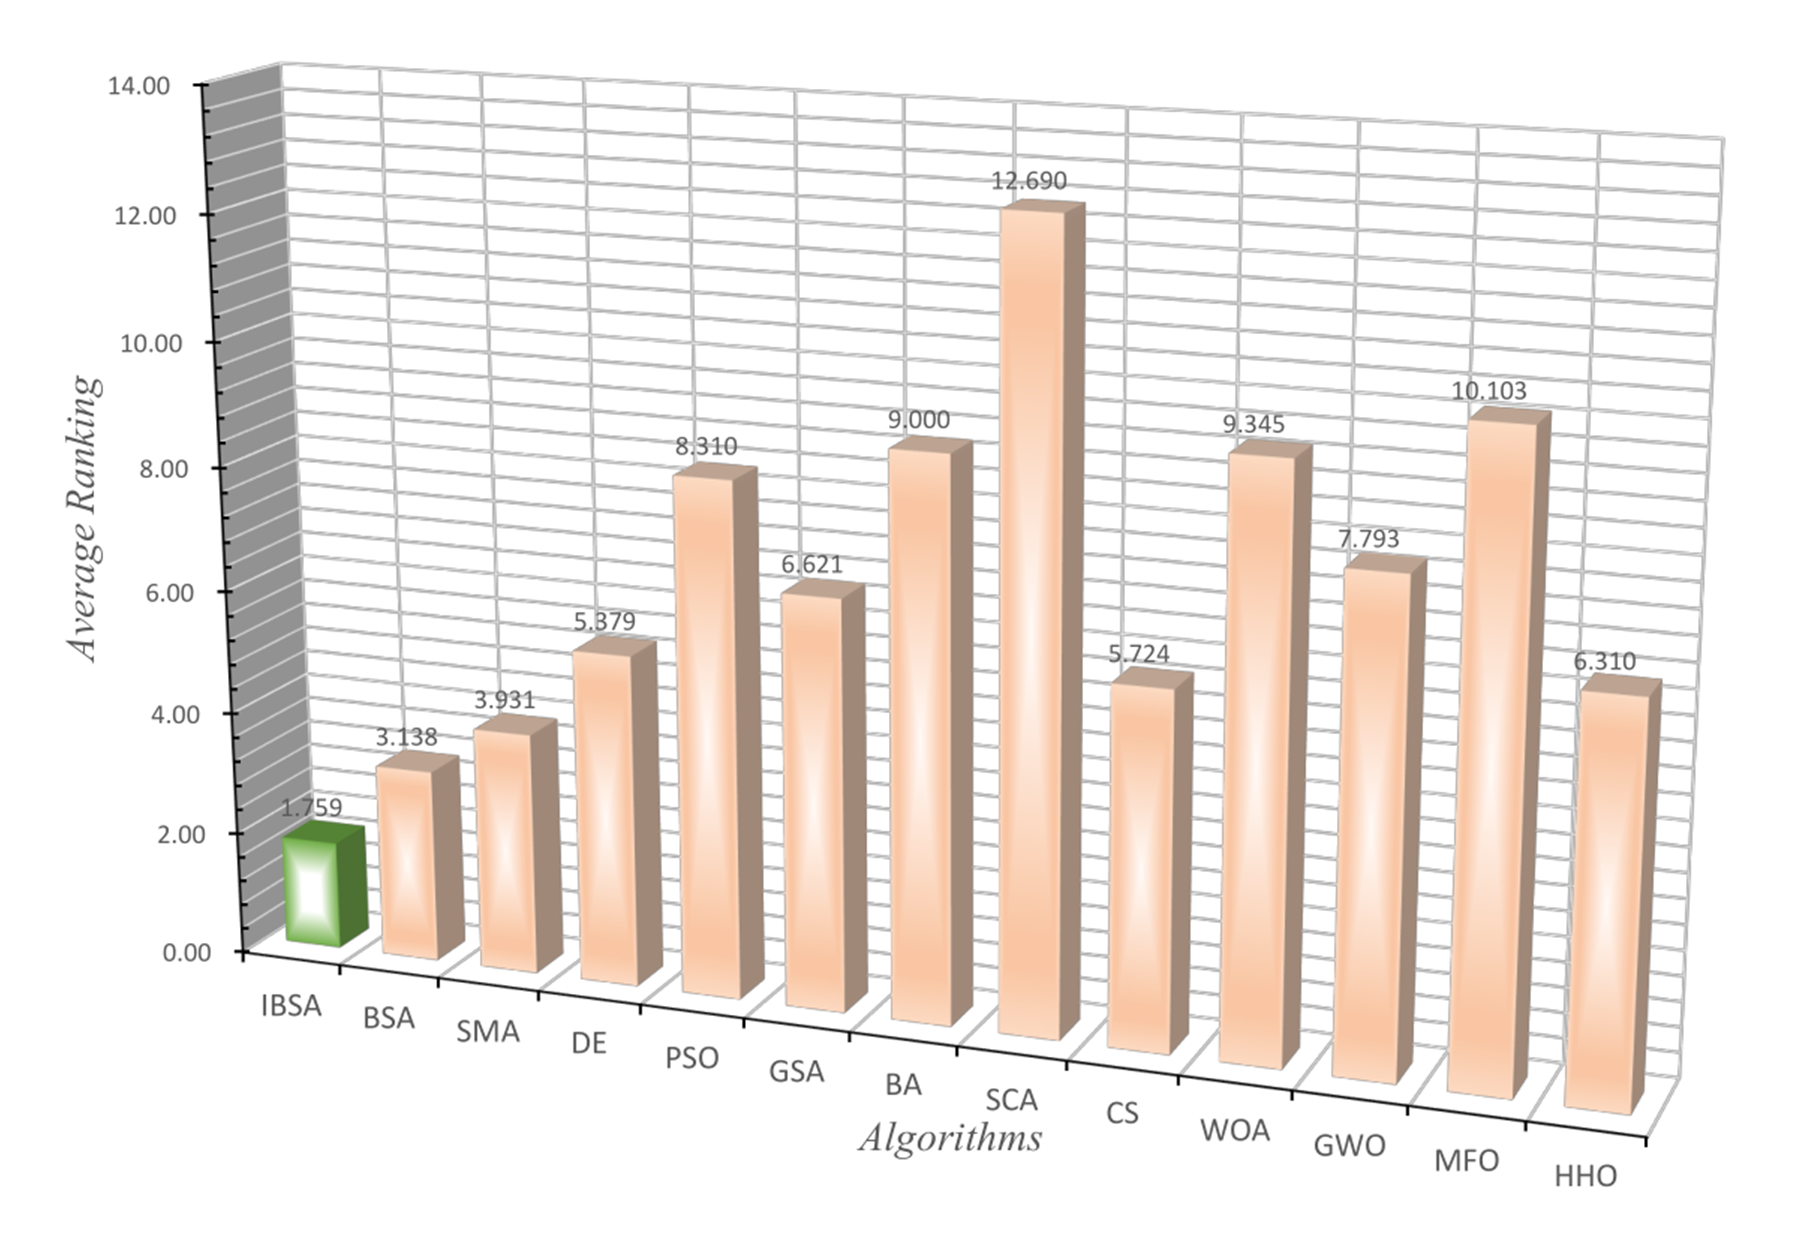
\includegraphics[width=\textwidth]{figures/fig5_friedman_ranking_basic.png}
  \caption{Average ranking of IBSA and the basic MAs.}
  \label{fig:friedman_ranking_basic}
\end{figure}



To better illustrate the effectiveness of the IBSA algorithm, two types of visual displays, namely the convergence curve and the box plot, are deployed in Fig. 6. These visuals focus on selected representative functions spanning all four types of problems encountered in the CEC 2017 function suite. The selected functions include the single-modal function F1, multi-modal functions F6 and F7, hybrid functions F12, F17, F18, F20, and composition functions F22, F23, and F27.

These functions exemplify the potent exploration and well-balanced capabilities of IBSA to converge and diversify when addressing disparate problems. The box plot further substantiates the robustness of our proposed IBSA. Aside from a slightly larger fluctuation in IBSA than BSA for the hybrid function F17, IBSA consistently maintains a superior average fitness value compared to BSA. This points towards the potent influence of the proposed elite leading mutation strategy on enhancing the overall performance of IBSA.

\begin{figure}[htbp]
  \centering
  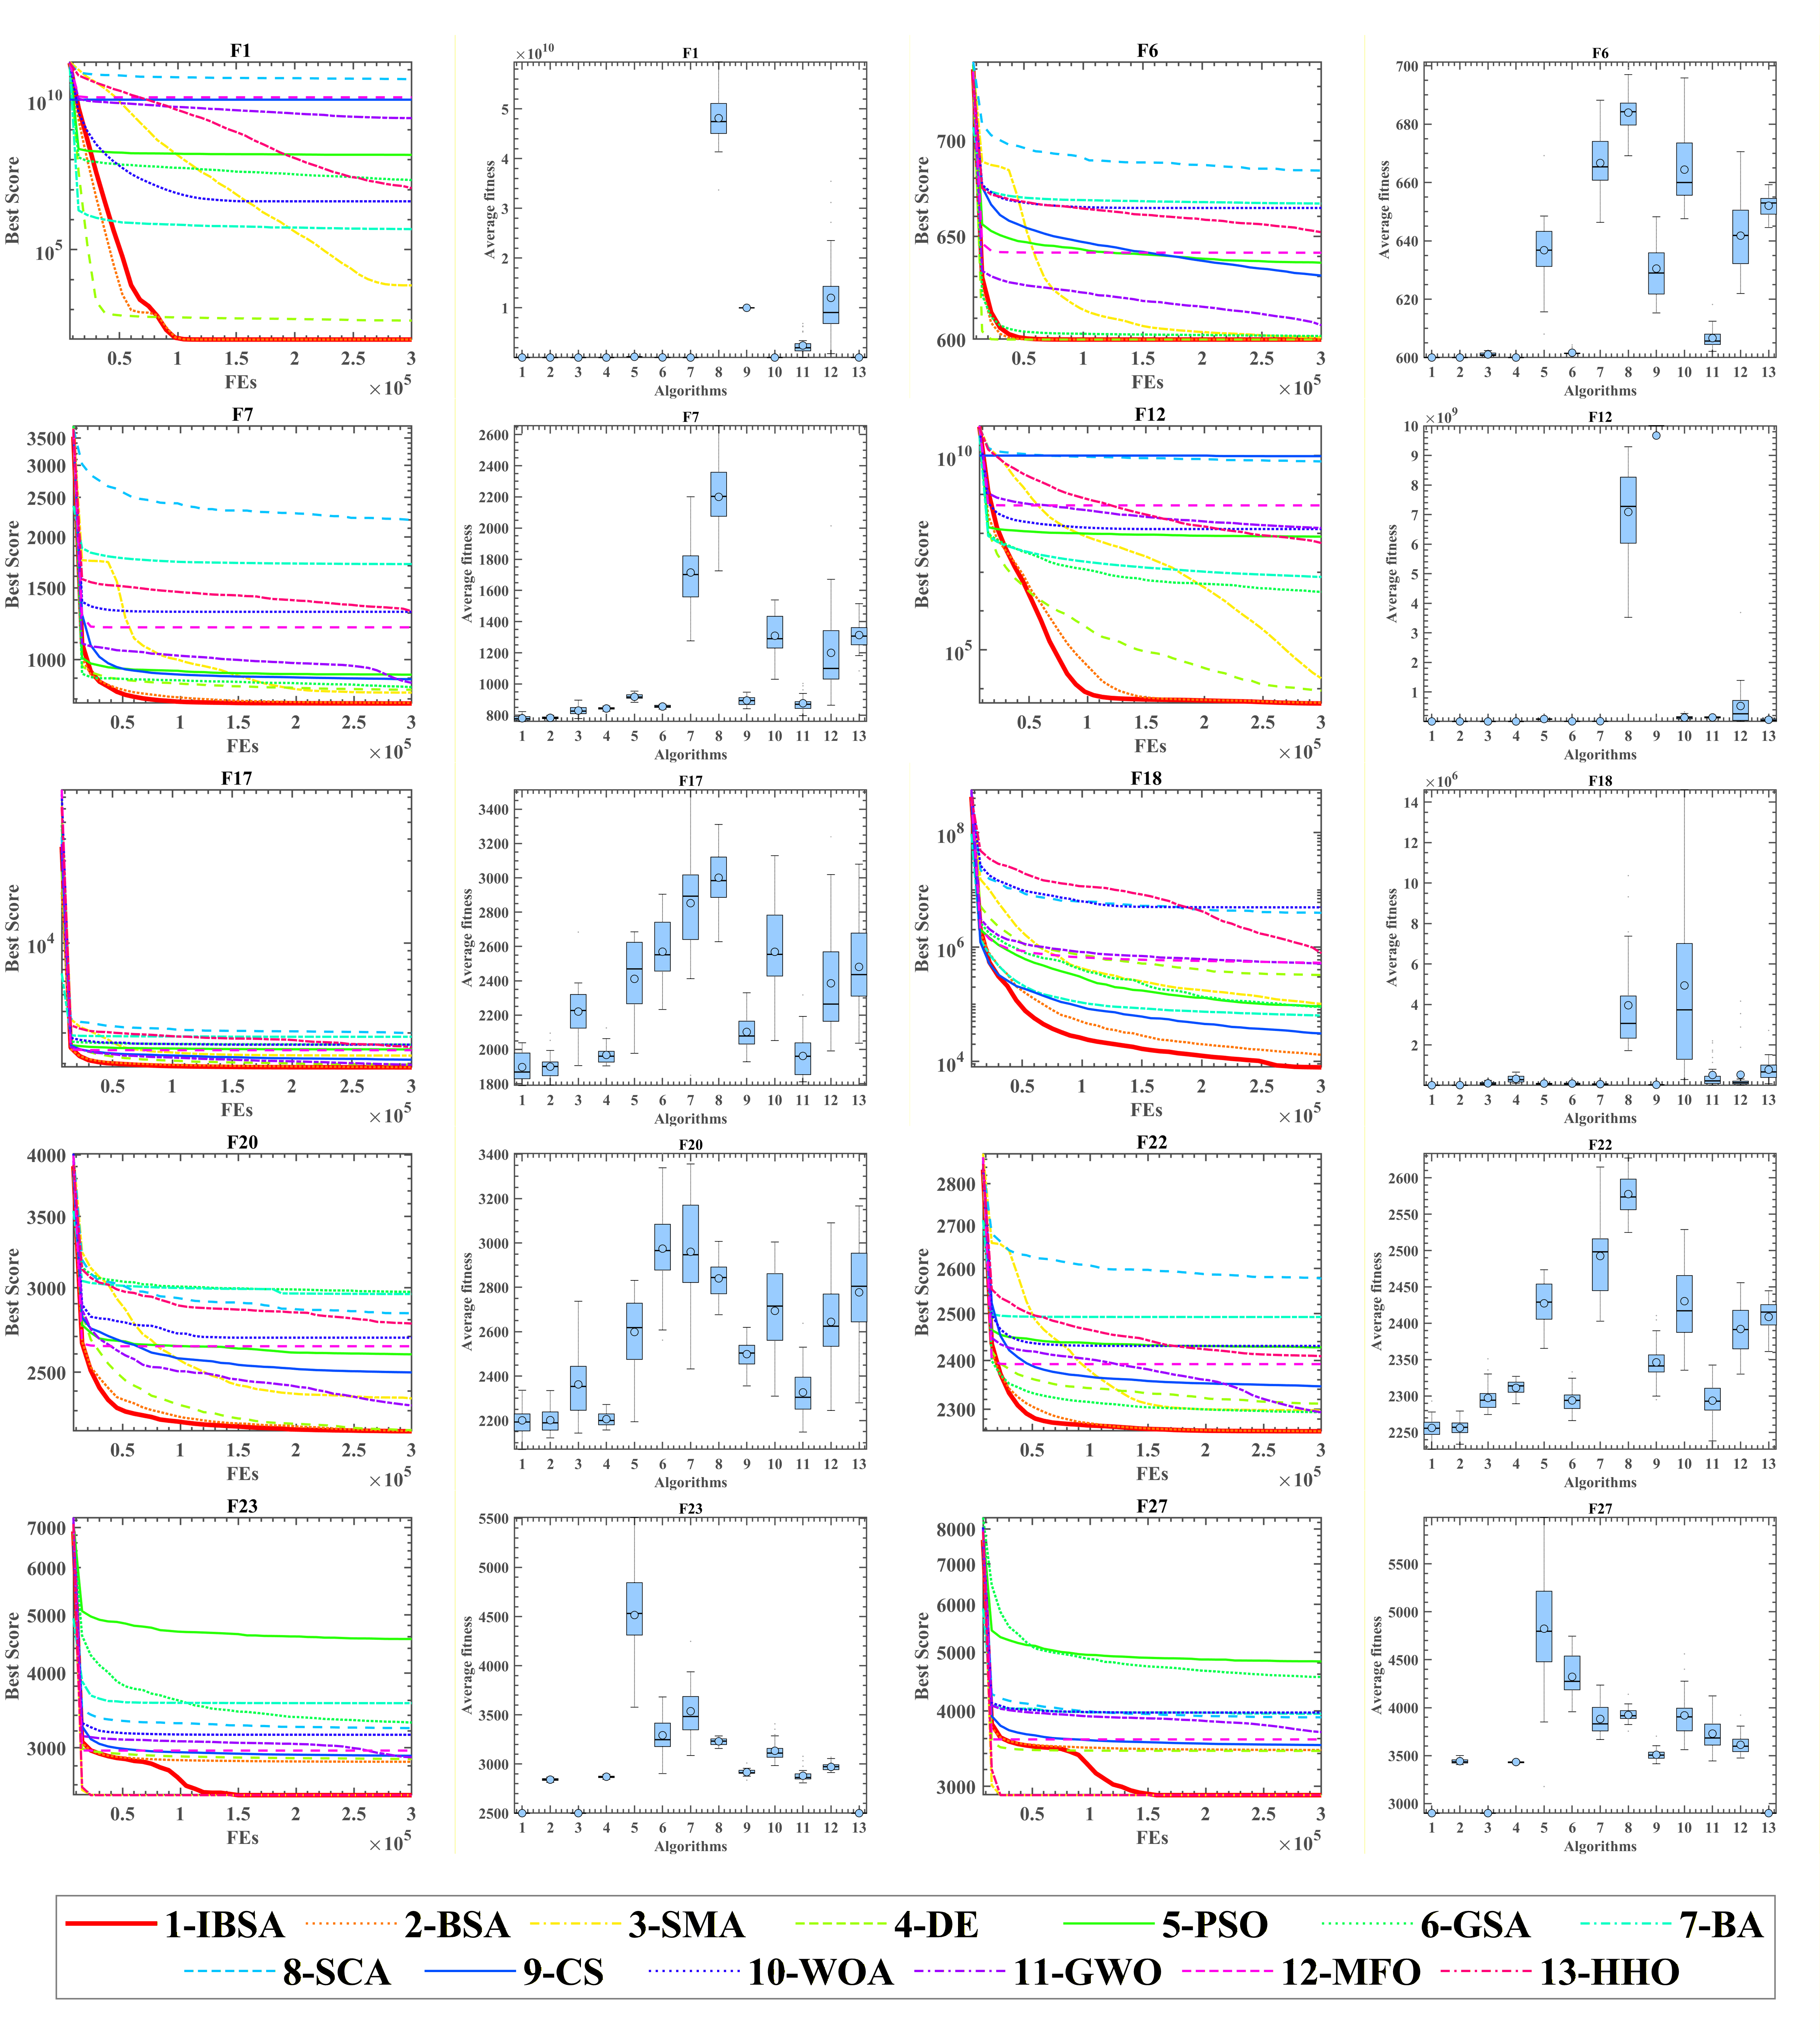
\includegraphics[width=\textwidth]{figures/fig6_convergence_basic_MAs.png}
  \caption{Convergence curves and box plots of the IBSA and other MAs on 10 functions.}
  \label{fig:convergence_basic_MAs}
\end{figure}




\paragraph{ Comparison with enhanced MAs variants}

This section is devoted to a meticulous comparison between our enhanced IBSA algorithm and other advanced swarm intelligence algorithms. The aim is to underscore the robust global optimization prowess of IBSA.

The algorithms selected for this comparison are as follows: Cooperatively Coevolving Particle Swarms Optimization (CGPSO) [84], Self-Adaptive Differential Evolution (SADE) [56], Reinforced Whale Optimization Algorithm (RDWOA) [68], Comprehensive Learning Particle Swarm Optimization (CLPSO) [85], Cross-Adaptive Gray Wolf Optimization (CAGWO) [86], Sine Cosine Algorithm Differential Evolution (SCADE) [87], Improved Gray Wolf Optimization (IGWO) [88], Differential Evolution based on Chaotic Local Search (DECLS) [89], PSO with Aging Leader and Challengers (ALCPSO) [90], Compact Bat Algorithm (CBA) [91], and Success-History Based Parameter Adaptation Differential Evolution (SHADE) [92].

Before delving into the statistical analysis, it is necessary to mention the outcomes summarized in Table 4, which evaluates the performance of our algorithm against these established ones using the IEEE CEC2017 function suite. The exceptional performance of IBSA is clearly presented in the last row of Table 4 using the Friedman test, where with an average ranking of 1.8621, it marks a significant superiority, being substantially lower than the second-ranked value of 3.9310. The demonstration of this superiority is further visualized through the average ranking chart of the Friedman test result depicted in Fig. 7.

Moving onto Table 5, this table employs the Wilcoxon signed-rank test to reinforce the comparative analysis. The results from this statistical test indicate that IBSA demonstrates significant advantages over a number of established algorithms. Specifically, IBSA outperforms CGPSO, SADE, RDWOA, CLPSO, CAGWO, SCADE, IGWO, DECLS, ALCPSO, CBA, and SHADE in several cases, achieving superiority in 26, 14, 22, 19, 27, 23, 28, 25, 28, 28, and 14 instances, respectively. The statistical significance of these outcomes is confirmed by the p-value, which is below 0.05, validating the overall dominance of IBSA.

However, there are instances when IBSA's performance aligns closely with that of the comparative algorithms. Specifically, with CGPSO, SADE, RDWOA, CLPSO, CAGWO, SCADE, IGWO, DECLS, ALCPSO, CBA, and SHADE, it exhibits comparable results in 2, 5, 0, 1, 0, 0, 1, 2, 0, 1, and 11 instances, respectively.

Nevertheless, there are minimal scenarios wherein IBSA slightly lags behind certain algorithms---namely CGPSO, SADE, RDWOA, CLPSO, CAGWO, SCADE, IGWO, DECLS, ALCPSO, and CBA---evidenced in 1, 10, 7, 9, 2, 6, 0, 2, 1, and 4 cases, respectively. The specific details of these performances are thoroughly elucidated in Table 5.

\begin{tabular}{|p{0.2in}|p{0.2in}|p{0.4in}|p{0.4in}|p{0.4in}|p{0.4in}|p{0.4in}|p{0.4in}|p{0.4in}|p{0.4in}|p{0.4in}|p{0.4in}|p{0.4in}|p{0.4in}|} \hline 
\multicolumn{13}{|p{4.5in}|}{\textbf{Table }4\textbf{. }Comparison results of IBSA and the advance MAs\textbf{}} & \textbf{} \\ \hline 
 & \textbf{Item} & \textbf{IBSA} & \textbf{CGPSO} & \textbf{SADE} & \textbf{RDWOA} & \textbf{CLPSO} & \textbf{CAGWO} & \textbf{SCADE} & \textbf{IGWO} & \textbf{DECLS} & \textbf{ALCPSO} & \textbf{CBA} & \textbf{SHADE} \\ \hline 
\textbf{F1} & Avg & \textbf{1.000E+02} & 1.513E+08 & 1.000E+02 & 2.211E+07 & 1.172E+02 & 2.855E+08 & 3.010E+10 & 3.010E+06 & 2.349E+02 & 1.645E+03 & 5.181E+05 & \textbf{1.000E+02} \\ \hline 
\textbf{} & Std & \textbf{4.571E-15} & 1.974E+07 & 8.989E-02 & 4.859E+07 & 4.038E+01 & 2.608E+08 & 6.428E+09 & 1.600E+06 & 5.536E+02 & 2.645E+03 & 1.991E+06 & 1.493E-14 \\ \hline 
\textbf{F3} & Avg & 1.801E+03 & 7.126E+02 & 4.564E+02 & 8.635E+03 & 8.668E+03 & 4.654E+04 & 6.228E+04 & 8.603E+02 & 5.511E+04 & 4.213E+03 & \textbf{3.173E+02} & 5.852E+03 \\ \hline 
\textbf{} & Std & 1.542E+03 & 5.413E+01 & 4.380E+02 & 4.218E+03 & 2.291E+03 & 6.564E+03 & 5.935E+03 & 2.529E+02 & 1.346E+04 & 5.833E+02 & \textbf{1.002E+01} & 1.920E+04 \\ \hline 
\textbf{F4} & Avg & 4.500E+02 & 4.656E+02 & 4.307E+02 & 5.443E+02 & 4.696E+02 & 5.795E+02 & 2.170E+03 & 5.337E+02 & 5.089E+02 & 5.104E+02 & 5.145E+02 & \textbf{4.021E+02} \\ \hline 
\textbf{} & Std & 2.935E+01 & 3.684E+01 & 3.353E+01 & 3.709E+01 & 2.270E+01 & 4.546E+01 & 4.792E+02 & 2.792E+01 & 1.831E+01 & 5.865E+01 & 3.371E+01 & \textbf{1.158E+01} \\ \hline 
\textbf{F~5} & Avg & 5.522E+02 & 7.048E+02 & 5.441E+02 & 6.688E+02 & 5.525E+02 & 6.259E+02 & 7.960E+02 & 5.934E+02 & 6.236E+02 & 5.840E+02 & 7.626E+02 & \textbf{5.335E+02} \\ \hline 
\textbf{} & Std & 1.299E+01 & 2.056E+01 & 1.185E+01 & 3.286E+01 & 1.057E+01 & 4.982E+01 & 1.455E+01 & 1.510E+01 & 1.125E+01 & 2.156E+01 & 6.227E+01 & \textbf{7.042E+00} \\ \hline 
\textbf{F6} & Avg & \textbf{6.000E+02} & 6.519E+02 & 6.000E+02 & 6.117E+02 & \textbf{6.000E+02} & 6.029E+02 & 6.591E+02 & 6.224E+02 & \textbf{6.000E+02} & 6.008E+02 & 6.678E+02 & 6.001E+02 \\ \hline 
\textbf{} & Std & 2.407E-13 & 8.368E+00 & 2.709E-02 & 5.624E+00 & 8.176E-14 & 1.335E+00 & 8.120E+00 & 4.228E+00 & \textbf{6.333E-14} & 6.327E-01 & 1.111E+01 & 4.898E-02 \\ \hline 
\textbf{F7} & Avg & 7.706E+02 & 9.266E+02 & 7.803E+02 & 9.927E+02 & 7.855E+02 & 9.164E+02 & 1.272E+03 & 8.980E+02 & 8.603E+02 & 8.514E+02 & 2.124E+03 & \textbf{7.627E+02} \\ \hline 
\textbf{} & Std & 1.054E+01 & 1.402E+01 & 1.303E+01 & 7.905E+01 & \textbf{6.401E+00} & 2.643E+01 & 3.793E+01 & 4.038E+01 & 9.097E+00 & 2.956E+01 & 3.479E+02 & 7.864E+00 \\ \hline 
\textbf{F8} & Avg & 8.436E+02 & 1.073E+03 & 8.464E+02 & 1.004E+03 & 8.479E+02 & 9.378E+02 & 1.116E+03 & 8.987E+02 & 9.253E+02 & 8.783E+02 & 1.118E+03 & \textbf{8.329E+02} \\ \hline 
\textbf{} & Std & 1.110E+01 & 3.384E+01 & 1.321E+01 & 4.039E+01 & 8.976E+00 & 4.698E+01 & 1.915E+01 & 2.242E+01 & 1.171E+01 & 2.034E+01 & 5.345E+01 & \textbf{8.454E+00} \\ \hline 
\textbf{F9} & Avg & 9.126E+02 & 8.024E+03 & 9.177E+02 & 6.302E+03 & 9.159E+02 & 1.170E+03 & 1.025E+04 & 3.379E+03 & \textbf{9.000E+02} & 1.239E+03 & 9.379E+03 & 9.213E+02 \\ \hline 
\textbf{} & Std & 1.551E+01 & 1.771E+03 & 1.571E+01 & 2.408E+03 & 1.229E+01 & 1.907E+02 & 1.163E+03 & 1.316E+03 & \textbf{3.657E-14} & 4.525E+02 & 2.542E+03 & 2.988E+01 \\ \hline 
\textbf{F10} & Avg & 2.943E+03 & 5.656E+03 & 2.952E+03 & 4.605E+03 & 3.011E+03 & 6.515E+03 & 7.352E+03 & 4.401E+03 & 6.172E+03 & 3.214E+03 & 5.389E+03 & \textbf{2.696E+03} \\ \hline 
\textbf{} & Std & 3.480E+02 & 5.614E+02 & 3.826E+02 & 5.376E+02 & 2.938E+02 & 1.582E+03 & 4.860E+02 & 7.162E+02 & 3.227E+02 & 5.498E+02 & 6.584E+02 & \textbf{2.443E+02} \\ \hline 
\textbf{F11} & Avg & \textbf{1.133E+03} & 1.391E+03 & 1.194E+03 & 1.296E+03 & 1.146E+03 & 1.868E+03 & 6.983E+03 & 1.323E+03 & 1.178E+03 & 1.181E+03 & 1.450E+03 & 1.268E+03 \\ \hline 
\textbf{} & Std & 1.764E+01 & 5.327E+01 & 4.882E+01 & 5.743E+01 & 1.114E+01 & 3.626E+02 & 1.031E+03 & 4.529E+01 & \textbf{1.034E+01} & 4.212E+01 & 1.514E+02 & 6.788E+01 \\ \hline 
\textbf{F12} & Avg & 4.009E+03 & 9.624E+07 & 5.122E+03 & 2.933E+07 & 4.608E+05 & 1.282E+08 & 2.702E+09 & 6.874E+07 & 1.354E+05 & 6.437E+03 & 4.535E+07 & \textbf{2.588E+03} \\ \hline 
\textbf{} & Std & 1.777E+03 & 3.733E+07 & 2.419E+03 & 2.220E+07 & 5.989E+05 & 3.483E+07 & 8.610E+08 & 2.727E+07 & 2.897E+05 & 3.346E+03 & 1.643E+07 & \textbf{3.461E+02} \\ \hline 
\textbf{F13} & Avg & \textbf{1.331E+03} & 2.935E+06 & 1.505E+03 & 3.927E+03 & 1.412E+03 & 1.252E+06 & 1.595E+08 & 6.521E+04 & 1.381E+03 & 1.642E+03 & 1.570E+05 & 1.444E+03 \\ \hline 
\textbf{} & Std & \textbf{7.205E+00} & 1.105E+06 & 2.843E+02 & 2.640E+03 & 4.992E+01 & 1.095E+06 & 6.839E+07 & 3.825E+04 & 8.608E+01 & 7.911E+02 & 1.227E+05 & 1.017E+02 \\ \hline 
\textbf{F14} & Avg & \textbf{1.436E+03} & 6.324E+04 & 1.559E+03 & 1.540E+04 & 4.082E+03 & 8.617E+04 & 4.401E+05 & 2.523E+04 & 1.495E+03 & 1.473E+03 & 3.856E+04 & 1.653E+03 \\ \hline 
\textbf{} & Std & \textbf{6.701E+00} & 3.775E+04 & 8.061E+01 & 5.181E+04 & 3.037E+03 & 7.861E+04 & 2.561E+05 & 2.864E+04 & 1.380E+01 & 2.713E+01 & 3.409E+04 & 1.055E+02 \\ \hline 
\textbf{F15} & Avg & \textbf{1.530E+03} & 3.824E+05 & 1.611E+03 & 4.157E+03 & 1.577E+03 & 1.982E+04 & 7.222E+06 & 2.840E+04 & 1.570E+03 & 1.608E+03 & 9.059E+04 & 1.630E+03 \\ \hline 
\textbf{} & Std & 2.020E+01 & 1.424E+05 & 1.135E+02 & 2.078E+03 & 3.131E+01 & 1.227E+04 & 4.255E+06 & 2.031E+04 & \textbf{1.618E+01} & 5.587E+01 & 1.083E+05 & 5.939E+01 \\ \hline 
\textbf{F16} & Avg & 2.108E+03 & 2.727E+03 & \textbf{1.922E+03} & 2.706E+03 & 1.993E+03 & 2.484E+03 & 3.544E+03 & 2.398E+03 & 2.137E+03 & 2.207E+03 & 3.333E+03 & 1.973E+03 \\ \hline 
\textbf{} & Std & 2.077E+02 & 3.344E+02 & 1.569E+02 & 3.346E+02 & \textbf{1.444E+02} & 3.469E+02 & 1.723E+02 & 2.695E+02 & 1.566E+02 & 2.651E+02 & 4.511E+02 & 1.535E+02 \\ \hline 
\textbf{F17} & Avg & 1.876E+03 & 2.430E+03 & \textbf{1.799E+03} & 2.140E+03 & 1.906E+03 & 1.958E+03 & 2.695E+03 & 2.024E+03 & 1.997E+03 & 1.992E+03 & 2.933E+03 & 1.879E+03 \\ \hline 
\textbf{} & Std & 7.437E+01 & 2.011E+02 & \textbf{3.730E+01} & 1.528E+02 & 4.785E+01 & 1.190E+02 & 2.181E+02 & 1.123E+02 & 4.737E+01 & 1.157E+02 & 3.828E+02 & 7.965E+01 \\ \hline 
\textbf{F18} & Avg & 1.006E+04 & 1.527E+05 & 1.156E+04 & 5.812E+05 & 1.154E+05 & 5.993E+05 & 2.297E+06 & 2.589E+05 & 7.576E+05 & 4.485E+04 & 8.849E+04 & \textbf{1.965E+03} \\ \hline 
\textbf{} & Std & 7.664E+03 & 7.361E+04 & 7.287E+03 & 6.815E+05 & 7.040E+04 & 5.093E+05 & 1.484E+06 & 2.421E+05 & 3.774E+05 & 2.472E+04 & 7.165E+04 & \textbf{5.919E+01} \\ \hline 
\textbf{F19} & Avg & \textbf{1.973E+03} & 3.930E+05 & 2.521E+03 & 7.155E+03 & 1.977E+03 & 3.027E+04 & 1.603E+07 & 6.746E+04 & 1.012E+04 & 8.888E+03 & 2.846E+05 & 2.028E+03 \\ \hline 
\textbf{} & Std & 9.369E+01 & 1.929E+05 & 1.029E+03 & 6.392E+03 & 7.155E+01 & 3.437E+04 & 6.553E+06 & 7.203E+04 & 8.268E+03 & 8.852E+03 & 2.384E+05 & \textbf{5.730E+01} \\ \hline 
\textbf{F20} & Avg & 2.206E+03 & 2.684E+03 & \textbf{2.106E+03} & 2.412E+03 & 2.224E+03 & 2.454E+03 & 2.835E+03 & 2.364E+03 & 2.268E+03 & 2.273E+03 & 3.019E+03 & 2.202E+03 \\ \hline 
 & Std & 8.782E+01 & 1.699E+02 & 5.720E+01 & 1.635E+02 & \textbf{5.505E+01} & 1.996E+02 & 9.600E+01 & 1.710E+02 & 5.610E+01 & 9.728E+01 & 2.498E+02 & 8.231E+01 \\ \hline 
\textbf{F21} & Avg\textbf{} & 2.155E+03 & 2.210E+03 & 2.170E+03 & 2.251E+03 & 2.181E+03 & 2.271E+03 & 4.636E+03 & 2.235E+03 & 2.199E+03 & 2.204E+03 & 2.215E+03 & \textbf{2.111E+03} \\ \hline 
\textbf{} & Std\textbf{} & 3.227E+01 & 4.170E+01 & 3.045E+01 & 2.838E+01 & \textbf{4.456E+00} & 3.137E+01 & 6.486E+02 & 1.961E+01 & 1.812E+01 & 4.084E+01 & 3.990E+01 & 2.750E+01 \\ \hline 
\textbf{F22} & Avg & 2.248E+03 & 2.448E+03 & 2.251E+03 & 2.395E+03 & 2.252E+03 & 2.320E+03 & 2.516E+03 & 2.299E+03 & 2.329E+03 & 2.285E+03 & 2.490E+03 & \textbf{2.233E+03} \\ \hline 
\textbf{} & Std & 1.196E+01 & 2.628E+01 & 1.402E+01 & 3.593E+01 & 8.377E+00 & 3.820E+01 & 1.698E+01 & 1.922E+01 & 1.074E+01 & 2.162E+01 & 5.675E+01 & \textbf{7.601E+00} \\ \hline 
\textbf{F23} & Avg & \textbf{2.500E+03} & 2.500E+03 & 2.840E+03 & 2.516E+03 & 2.843E+03 & 2.896E+03 & 3.015E+03 & 2.918E+03 & 2.527E+03 & 2.995E+03 & 3.520E+03 & 2.830E+03 \\ \hline 
\textbf{} & Std & \textbf{0.000E+00} & 1.419E-04 & 2.042E+01 & 8.711E+01 & 9.217E+00 & 4.891E+01 & 3.841E+02 & 3.743E+01 & 1.040E+02 & 9.808E+01 & 2.723E+02 & 1.222E+01 \\ \hline 
\textbf{F24} & Avg & \textbf{2.600E+03} & 2.600E+03 & 2.600E+03 & \textbf{2.600E+03} & 2.610E+03 & 2.625E+03 & \textbf{2.600E+03} & 3.418E+03 & 2.600E+03 & 3.082E+03 & 2.969E+03 & 3.189E+03 \\ \hline 
\textbf{} & Std & \textbf{0.000E+00} & 2.214E-04 & 1.355E+00 & \textbf{0.000E+00} & 1.057E+01 & 9.593E+01 & \textbf{0.000E+00} & 1.479E+02 & 1.600E-04 & 4.213E+02 & 6.262E+02 & 3.157E+02 \\ \hline 
\textbf{F25} & Avg & \textbf{2.700E+03} & 2.700E+03 & 3.005E+03 & \textbf{2.700E+03} & 2.912E+03 & 2.784E+03 & \textbf{2.700E+03} & 2.983E+03 & 2.700E+03 & 2.979E+03 & 3.016E+03 & 2.934E+03 \\ \hline 
\textbf{} & Std & \textbf{0.000E+00} & 5.961E-03 & 5.954E+01 & \textbf{0.000E+00} & 1.388E+01 & 1.707E+02 & \textbf{0.000E+00} & 9.016E+01 & 3.550E-03 & 4.992E+01 & 8.495E+01 & 4.929E+01 \\ \hline 
\textbf{F26} & Avg & \textbf{2.800E+03} & 2.800E+03 & 2.884E+03 & \textbf{2.800E+03} & 3.650E+03 & 3.197E+03 & \textbf{2.800E+03} & 5.485E+03 & 2.800E+03 & 4.969E+03 & 5.233E+03 & 4.320E+03 \\ \hline 
\textbf{} & Std & \textbf{0.000E+00} & 5.514E-03 & 4.434E+02 & \textbf{0.000E+00} & 6.753E+02 & 9.051E+02 & \textbf{0.000E+00} & 6.375E+02 & 2.993E-03 & 1.207E+03 & 3.630E+03 & 8.419E+02 \\ \hline 
\textbf{F27} & Avg & \textbf{2.900E+03} & 3.002E+03 & 3.477E+03 & 2.948E+03 & 3.510E+03 & 3.519E+03 & 3.987E+03 & 3.610E+03 & 2.989E+03 & 3.802E+03 & 3.926E+03 & 3.545E+03 \\ \hline 
\textbf{} & Std & \textbf{0.000E+00} & 4.222E+02 & 4.545E+01 & 1.837E+02 & 3.391E+01 & 6.544E+01 & 2.310E+02 & 8.039E+01 & 2.032E+02 & 1.683E+02 & 2.750E+02 & 7.453E+01 \\ \hline 
\textbf{F28} & Avg & \textbf{3.000E+03} & 3.000E+03 & 3.277E+03 & 3.008E+03 & 3.280E+03 & 3.504E+03 & \textbf{3.000E+03} & 4.580E+03 & 3.000E+03 & 3.290E+03 & 3.576E+03 & 3.273E+03 \\ \hline 
\textbf{} & Std & \textbf{0.000E+00} & 8.377E-03 & 3.015E+01 & 4.497E+01 & 1.788E+01 & 1.206E+02 & \textbf{0.000E+00} & 9.419E+02 & 7.041E-03 & 5.067E+01 & 7.544E+02 & 6.532E+01 \\ \hline 
\textbf{F29} & Avg & \textbf{3.100E+03} & 3.100E+03 & 3.282E+03 & 3.124E+03 & 3.362E+03 & 3.369E+03 & \textbf{3.100E+03} & 3.681E+03 & 3.100E+03 & 3.472E+03 & 4.964E+03 & 3.334E+03 \\ \hline 
\textbf{} & Std & \textbf{0.000E+00} & 9.763E-03 & 5.696E+01 & 1.110E+02 & 7.254E+01 & 1.065E+02 & \textbf{0.000E+00} & 1.848E+02 & 2.550E-01 & 1.279E+02 & 4.141E+02 & 7.782E+01 \\ \hline 
\textbf{F30} & Avg & 6.643E+03 & 4.218E+03 & 7.077E+03 & 8.387E+04 & 1.499E+04 & 4.050E+05 & 1.681E+05 & 7.269E+05 & \textbf{4.007E+03} & 5.013E+04 & 2.534E+06 & 4.154E+03 \\ \hline 
\textbf{} & Std & 2.515E+03 & 1.087E+03 & 3.225E+03 & 4.883E+04 & 8.575E+03 & 2.219E+05 & 4.378E+05 & 9.008E+05 & 1.162E+03 & 5.328E+04 & 1.490E+06 & \textbf{2.008E+02} \\ \hline 
\textbf{} & \textbf{+/-/=} & $\mathrm{\sim}$ & 26/2/1 & 14/5/10 & 22/0/7 & 19/1/9 & 27/0/2 & 23/0/6 & 28/1/0 & 25/2/2 & 28/0/1 & 28/1/0 & 14/11/4 \\ \hline 
\textbf{} & Avg & 1.8621  & 7.6552  & 4.0000  & 6.8621  & 4.8966  & 8.7586  & 9.7931  & 8.4483  & 4.9655  & 6.4138  & 9.8966  & 3.9310  \\ \hline 
\textbf{} & Rank & 1 & 8 & 2 & 7 & 5 & 10 & 11 & 9 & 4 & 6 & 12 & 2 \\ \hline 
\end{tabular}



\begin{tabular}{|p{0.3in}|p{0.2in}|p{0.3in}|p{0.2in}|p{0.1in}|p{0.3in}|p{0.3in}|p{0.2in}|p{0.6in}|p{0.1in}|p{0.2in}|p{0.3in}|p{0.3in}|p{0.1in}|p{0.1in}|p{0.4in}|p{0.2in}|p{0.1in}|p{0.1in}|p{0.5in}|p{0.2in}|p{0.2in}|} \hline 
\multicolumn{22}{|p{5.3in}|}{\textbf{Table }5\textbf{. }P-value of Wilcoxon test obtained from comparison with advance MAs} \\ \hline 
Fun & \multicolumn{4}{|p{0.8in}|}{IBSA vs CGPSO} & \multicolumn{3}{|p{0.8in}|}{IBSA vs SADE} & \multicolumn{3}{|p{1.0in}|}{IBSA vs RDWOA} & \multicolumn{4}{|p{0.9in}|}{IBSA vs CLPSO} & \multicolumn{4}{|p{0.8in}|}{IBSA vs CAGWO} & \multicolumn{3}{|p{0.9in}|}{IBSA vs SCADE} \\ \hline 
 & \multicolumn{2}{|p{0.6in}|}{p-Value} & \multicolumn{2}{|p{0.3in}|}{} & \multicolumn{2}{|p{0.6in}|}{p-Value} &  & \multicolumn{2}{|p{0.7in}|}{p-Value} &  & \multicolumn{2}{|p{0.6in}|}{p-Value} & \multicolumn{2}{|p{0.3in}|}{} & \multicolumn{2}{|p{0.6in}|}{p-Value} & \multicolumn{2}{|p{0.3in}|}{} & \multicolumn{2}{|p{0.6in}|}{p-Value} &  \\ \hline 
\textbf{F1} & \multicolumn{2}{|p{0.6in}|}{1.734E-06} & \multicolumn{2}{|p{0.3in}|}{+} & \multicolumn{2}{|p{0.6in}|}{2.902E-04} & + & \multicolumn{2}{|p{0.7in}|}{1.734E-06} & + & \multicolumn{2}{|p{0.6in}|}{1.733E-06} & \multicolumn{2}{|p{0.3in}|}{+} & \multicolumn{2}{|p{0.6in}|}{1.733E-06} & \multicolumn{2}{|p{0.3in}|}{+} & \multicolumn{2}{|p{0.6in}|}{1.733E-06} & + \\ \hline 
\textbf{F3} & \multicolumn{2}{|p{0.6in}|}{2.163E-05} & \multicolumn{2}{|p{0.3in}|}{-} & \multicolumn{2}{|p{0.6in}|}{2.597E-05} & - & \multicolumn{2}{|p{0.7in}|}{1.921E-06} & + & \multicolumn{2}{|p{0.6in}|}{1.734E-06} & \multicolumn{2}{|p{0.3in}|}{+} & \multicolumn{2}{|p{0.6in}|}{1.734E-06} & \multicolumn{2}{|p{0.3in}|}{+} & \multicolumn{2}{|p{0.6in}|}{1.734E-06} & + \\ \hline 
\textbf{F4} & \multicolumn{2}{|p{0.6in}|}{5.170E-01} & \multicolumn{2}{|p{0.3in}|}{ =} & \multicolumn{2}{|p{0.6in}|}{5.984E-02} &  = & \multicolumn{2}{|p{0.7in}|}{1.734E-06} & + & \multicolumn{2}{|p{0.6in}|}{2.067E-02} & \multicolumn{2}{|p{0.3in}|}{+} & \multicolumn{2}{|p{0.6in}|}{1.734E-06} & \multicolumn{2}{|p{0.3in}|}{+} & \multicolumn{2}{|p{0.6in}|}{1.734E-06} & + \\ \hline 
\textbf{F5} & \multicolumn{2}{|p{0.6in}|}{1.734E-06} & \multicolumn{2}{|p{0.3in}|}{+} & \multicolumn{2}{|p{0.6in}|}{1.480E-02} & - & \multicolumn{2}{|p{0.7in}|}{1.734E-06} & + & \multicolumn{2}{|p{0.6in}|}{9.754E-01} & \multicolumn{2}{|p{0.3in}|}{ =} & \multicolumn{2}{|p{0.6in}|}{2.353E-06} & \multicolumn{2}{|p{0.3in}|}{+} & \multicolumn{2}{|p{0.6in}|}{1.734E-06} & + \\ \hline 
\textbf{F6} & \multicolumn{2}{|p{0.6in}|}{1.734E-06} & \multicolumn{2}{|p{0.3in}|}{+} & \multicolumn{2}{|p{0.6in}|}{1.176E-05} & + & \multicolumn{2}{|p{0.7in}|}{1.734E-06} & + & \multicolumn{2}{|p{0.6in}|}{6.250E-02} & \multicolumn{2}{|p{0.3in}|}{ =} & \multicolumn{2}{|p{0.6in}|}{1.734E-06} & \multicolumn{2}{|p{0.3in}|}{+} & \multicolumn{2}{|p{0.6in}|}{1.734E-06} & + \\ \hline 
\textbf{F7} & \multicolumn{2}{|p{0.6in}|}{1.734E-06} & \multicolumn{2}{|p{0.3in}|}{+} & \multicolumn{2}{|p{0.6in}|}{8.307E-04} & + & \multicolumn{2}{|p{0.7in}|}{1.734E-06} & + & \multicolumn{2}{|p{0.6in}|}{3.112E-05} & \multicolumn{2}{|p{0.3in}|}{+} & \multicolumn{2}{|p{0.6in}|}{1.734E-06} & \multicolumn{2}{|p{0.3in}|}{+} & \multicolumn{2}{|p{0.6in}|}{1.734E-06} & + \\ \hline 
\textbf{F8} & \multicolumn{2}{|p{0.6in}|}{1.734E-06} & \multicolumn{2}{|p{0.3in}|}{+} & \multicolumn{2}{|p{0.6in}|}{2.452E-01} &  = & \multicolumn{2}{|p{0.7in}|}{1.734E-06} & + & \multicolumn{2}{|p{0.6in}|}{1.204E-01} & \multicolumn{2}{|p{0.3in}|}{ =} & \multicolumn{2}{|p{0.6in}|}{2.127E-06} & \multicolumn{2}{|p{0.3in}|}{+} & \multicolumn{2}{|p{0.6in}|}{1.734E-06} & + \\ \hline 
\textbf{F9} & \multicolumn{2}{|p{0.6in}|}{1.734E-06} & \multicolumn{2}{|p{0.3in}|}{+} & \multicolumn{2}{|p{0.6in}|}{8.972E-02} &  = & \multicolumn{2}{|p{0.7in}|}{1.734E-06} & + & \multicolumn{2}{|p{0.6in}|}{1.529E-01} & \multicolumn{2}{|p{0.3in}|}{ =} & \multicolumn{2}{|p{0.6in}|}{1.734E-06} & \multicolumn{2}{|p{0.3in}|}{+} & \multicolumn{2}{|p{0.6in}|}{1.734E-06} & + \\ \hline 
\textbf{F10} & \multicolumn{2}{|p{0.6in}|}{1.734E-06} & \multicolumn{2}{|p{0.3in}|}{+} & \multicolumn{2}{|p{0.6in}|}{8.290E-01} &  = & \multicolumn{2}{|p{0.7in}|}{1.734E-06} & + & \multicolumn{2}{|p{0.6in}|}{9.777E-02} & \multicolumn{2}{|p{0.3in}|}{ =} & \multicolumn{2}{|p{0.6in}|}{2.353E-06} & \multicolumn{2}{|p{0.3in}|}{+} & \multicolumn{2}{|p{0.6in}|}{1.734E-06} & + \\ \hline 
\textbf{F11} & \multicolumn{2}{|p{0.6in}|}{1.734E-06} & \multicolumn{2}{|p{0.3in}|}{+} & \multicolumn{2}{|p{0.6in}|}{6.984E-06} & + & \multicolumn{2}{|p{0.7in}|}{1.734E-06} & + & \multicolumn{2}{|p{0.6in}|}{3.379E-03} & \multicolumn{2}{|p{0.3in}|}{+} & \multicolumn{2}{|p{0.6in}|}{1.734E-06} & \multicolumn{2}{|p{0.3in}|}{+} & \multicolumn{2}{|p{0.6in}|}{1.734E-06} & + \\ \hline 
\textbf{F12} & \multicolumn{2}{|p{0.6in}|}{1.734E-06} & \multicolumn{2}{|p{0.3in}|}{+} & \multicolumn{2}{|p{0.6in}|}{3.683E-02} & + & \multicolumn{2}{|p{0.7in}|}{1.734E-06} & + & \multicolumn{2}{|p{0.6in}|}{1.921E-06} & \multicolumn{2}{|p{0.3in}|}{+} & \multicolumn{2}{|p{0.6in}|}{1.734E-06} & \multicolumn{2}{|p{0.3in}|}{+} & \multicolumn{2}{|p{0.6in}|}{1.734E-06} & + \\ \hline 
\textbf{F13} & \multicolumn{2}{|p{0.6in}|}{1.734E-06} & \multicolumn{2}{|p{0.3in}|}{+} & \multicolumn{2}{|p{0.6in}|}{1.734E-06} & + & \multicolumn{2}{|p{0.7in}|}{1.734E-06} & + & \multicolumn{2}{|p{0.6in}|}{1.734E-06} & \multicolumn{2}{|p{0.3in}|}{+} & \multicolumn{2}{|p{0.6in}|}{1.734E-06} & \multicolumn{2}{|p{0.3in}|}{+} & \multicolumn{2}{|p{0.6in}|}{1.734E-06} & + \\ \hline 
\textbf{F14} & \multicolumn{2}{|p{0.6in}|}{1.734E-06} & \multicolumn{2}{|p{0.3in}|}{+} & \multicolumn{2}{|p{0.6in}|}{1.734E-06} & + & \multicolumn{2}{|p{0.7in}|}{1.734E-06} & + & \multicolumn{2}{|p{0.6in}|}{1.734E-06} & \multicolumn{2}{|p{0.3in}|}{+} & \multicolumn{2}{|p{0.6in}|}{1.734E-06} & \multicolumn{2}{|p{0.3in}|}{+} & \multicolumn{2}{|p{0.6in}|}{1.734E-06} & + \\ \hline 
\textbf{F15} & \multicolumn{2}{|p{0.6in}|}{1.734E-06} & \multicolumn{2}{|p{0.3in}|}{+} & \multicolumn{2}{|p{0.6in}|}{1.025E-05} & + & \multicolumn{2}{|p{0.7in}|}{1.734E-06} & + & \multicolumn{2}{|p{0.6in}|}{1.360E-05} & \multicolumn{2}{|p{0.3in}|}{+} & \multicolumn{2}{|p{0.6in}|}{1.734E-06} & \multicolumn{2}{|p{0.3in}|}{+} & \multicolumn{2}{|p{0.6in}|}{1.734E-06} & + \\ \hline 
\textbf{F16} & \multicolumn{2}{|p{0.6in}|}{4.286E-06} & \multicolumn{2}{|p{0.3in}|}{+} & \multicolumn{2}{|p{0.6in}|}{1.197E-03} & - & \multicolumn{2}{|p{0.7in}|}{2.353E-06} & + & \multicolumn{2}{|p{0.6in}|}{9.842E-03} & \multicolumn{2}{|p{0.3in}|}{-} & \multicolumn{2}{|p{0.6in}|}{3.065E-04} & \multicolumn{2}{|p{0.3in}|}{+} & \multicolumn{2}{|p{0.6in}|}{1.734E-06} & + \\ \hline 
\textbf{F17} & \multicolumn{2}{|p{0.6in}|}{1.734E-06} & \multicolumn{2}{|p{0.3in}|}{+} & \multicolumn{2}{|p{0.6in}|}{4.449E-05} & - & \multicolumn{2}{|p{0.7in}|}{2.353E-06} & + & \multicolumn{2}{|p{0.6in}|}{5.193E-02} & \multicolumn{2}{|p{0.3in}|}{ =} & \multicolumn{2}{|p{0.6in}|}{1.108E-02} & \multicolumn{2}{|p{0.3in}|}{+} & \multicolumn{2}{|p{0.6in}|}{1.734E-06} & + \\ \hline 
\textbf{F18} & \multicolumn{2}{|p{0.6in}|}{1.734E-06} & \multicolumn{2}{|p{0.3in}|}{+} & \multicolumn{2}{|p{0.6in}|}{1.156E-01} &  = & \multicolumn{2}{|p{0.7in}|}{1.734E-06} & + & \multicolumn{2}{|p{0.6in}|}{1.734E-06} & \multicolumn{2}{|p{0.3in}|}{+} & \multicolumn{2}{|p{0.6in}|}{1.734E-06} & \multicolumn{2}{|p{0.3in}|}{+} & \multicolumn{2}{|p{0.6in}|}{1.734E-06} & + \\ \hline 
\textbf{F19} & \multicolumn{2}{|p{0.6in}|}{1.734E-06} & \multicolumn{2}{|p{0.3in}|}{+} & \multicolumn{2}{|p{0.6in}|}{5.307E-05} & + & \multicolumn{2}{|p{0.7in}|}{1.734E-06} & + & \multicolumn{2}{|p{0.6in}|}{2.802E-01} & \multicolumn{2}{|p{0.3in}|}{ =} & \multicolumn{2}{|p{0.6in}|}{1.734E-06} & \multicolumn{2}{|p{0.3in}|}{+} & \multicolumn{2}{|p{0.6in}|}{1.734E-06} & + \\ \hline 
\textbf{F20} & \multicolumn{2}{|p{0.6in}|}{1.734E-06} & \multicolumn{2}{|p{0.3in}|}{+} & \multicolumn{2}{|p{0.6in}|}{1.359E-04} & - & \multicolumn{2}{|p{0.7in}|}{7.691E-06} & + & \multicolumn{2}{|p{0.6in}|}{4.528E-01} & \multicolumn{2}{|p{0.3in}|}{ =} & \multicolumn{2}{|p{0.6in}|}{1.238E-05} & \multicolumn{2}{|p{0.3in}|}{+} & \multicolumn{2}{|p{0.6in}|}{1.734E-06} & + \\ \hline 
\textbf{F21} & \multicolumn{2}{|p{0.6in}|}{7.514E-05} & \multicolumn{2}{|p{0.3in}|}{+} & \multicolumn{2}{|p{0.6in}|}{1.779E-01} &  = & \multicolumn{2}{|p{0.7in}|}{1.734E-06} & + & \multicolumn{2}{|p{0.6in}|}{2.370E-05} & \multicolumn{2}{|p{0.3in}|}{+} & \multicolumn{2}{|p{0.6in}|}{1.734E-06} & \multicolumn{2}{|p{0.3in}|}{+} & \multicolumn{2}{|p{0.6in}|}{1.734E-06} & + \\ \hline 
\textbf{F22} & \multicolumn{2}{|p{0.6in}|}{1.734E-06} & \multicolumn{2}{|p{0.3in}|}{+} & \multicolumn{2}{|p{0.6in}|}{4.048E-01} &  = & \multicolumn{2}{|p{0.7in}|}{1.734E-06} & + & \multicolumn{2}{|p{0.6in}|}{1.846E-01} & \multicolumn{2}{|p{0.3in}|}{ =} & \multicolumn{2}{|p{0.6in}|}{2.603E-06} & \multicolumn{2}{|p{0.3in}|}{+} & \multicolumn{2}{|p{0.6in}|}{1.734E-06} & + \\ \hline 
\textbf{F23} & \multicolumn{2}{|p{0.6in}|}{1.734E-06} & \multicolumn{2}{|p{0.3in}|}{+} & \multicolumn{2}{|p{0.6in}|}{1.734E-06} & + & \multicolumn{2}{|p{0.7in}|}{1.000E+00} & =  & \multicolumn{2}{|p{0.6in}|}{1.734E-06} & \multicolumn{2}{|p{0.3in}|}{+} & \multicolumn{2}{|p{0.6in}|}{1.734E-06} & \multicolumn{2}{|p{0.3in}|}{+} & \multicolumn{2}{|p{0.6in}|}{8.857E-05} & + \\ \hline 
\textbf{F24} & \multicolumn{2}{|p{0.6in}|}{1.734E-06} & \multicolumn{2}{|p{0.3in}|}{+} & \multicolumn{2}{|p{0.6in}|}{5.000E-01} &  = & \multicolumn{2}{|p{0.7in}|}{1.000E+00} & =  & \multicolumn{2}{|p{0.6in}|}{1.734E-06} & \multicolumn{2}{|p{0.3in}|}{+} & \multicolumn{2}{|p{0.6in}|}{5.000E-01} & \multicolumn{2}{|p{0.3in}|}{ =} & \multicolumn{2}{|p{0.6in}|}{1.000E+00} &  = \\ \hline 
\textbf{F25} & \multicolumn{2}{|p{0.6in}|}{1.734E-06} & \multicolumn{2}{|p{0.3in}|}{+} & \multicolumn{2}{|p{0.6in}|}{1.734E-06} & + & \multicolumn{2}{|p{0.7in}|}{1.000E+00} & =  & \multicolumn{2}{|p{0.6in}|}{1.733E-06} & \multicolumn{2}{|p{0.3in}|}{+} & \multicolumn{2}{|p{0.6in}|}{3.125E-02} & \multicolumn{2}{|p{0.3in}|}{+} & \multicolumn{2}{|p{0.6in}|}{1.000E+00} &  = \\ \hline 
\textbf{F26} & \multicolumn{2}{|p{0.6in}|}{1.734E-06} & \multicolumn{2}{|p{0.3in}|}{+} & \multicolumn{2}{|p{0.6in}|}{5.000E-01} &  = & \multicolumn{2}{|p{0.7in}|}{1.000E+00} & =  & \multicolumn{2}{|p{0.6in}|}{1.733E-06} & \multicolumn{2}{|p{0.3in}|}{+} & \multicolumn{2}{|p{0.6in}|}{6.250E-02} & \multicolumn{2}{|p{0.3in}|}{ =} & \multicolumn{2}{|p{0.6in}|}{1.000E+00} &  = \\ \hline 
\textbf{F27} & \multicolumn{2}{|p{0.6in}|}{1.734E-06} & \multicolumn{2}{|p{0.3in}|}{+} & \multicolumn{2}{|p{0.6in}|}{1.734E-06} & + & \multicolumn{2}{|p{0.7in}|}{5.000E-01} & =  & \multicolumn{2}{|p{0.6in}|}{1.733E-06} & \multicolumn{2}{|p{0.3in}|}{+} & \multicolumn{2}{|p{0.6in}|}{1.733E-06} & \multicolumn{2}{|p{0.3in}|}{+} & \multicolumn{2}{|p{0.6in}|}{1.733E-06} & + \\ \hline 
\textbf{F28} & \multicolumn{2}{|p{0.6in}|}{1.734E-06} & \multicolumn{2}{|p{0.3in}|}{+} & \multicolumn{2}{|p{0.6in}|}{1.734E-06} & + & \multicolumn{2}{|p{0.7in}|}{1.000E+00} & =  & \multicolumn{2}{|p{0.6in}|}{1.733E-06} & \multicolumn{2}{|p{0.3in}|}{+} & \multicolumn{2}{|p{0.6in}|}{1.733E-06} & \multicolumn{2}{|p{0.3in}|}{+} & \multicolumn{2}{|p{0.6in}|}{1.000E+00} &  = \\ \hline 
\textbf{F29} & \multicolumn{2}{|p{0.6in}|}{1.734E-06} & \multicolumn{2}{|p{0.3in}|}{+} & \multicolumn{2}{|p{0.6in}|}{1.734E-06} & + & \multicolumn{2}{|p{0.7in}|}{5.000E-01} & =  & \multicolumn{2}{|p{0.6in}|}{1.734E-06} & \multicolumn{2}{|p{0.3in}|}{+} & \multicolumn{2}{|p{0.6in}|}{2.563E-06} & \multicolumn{2}{|p{0.3in}|}{+} & \multicolumn{2}{|p{0.6in}|}{1.000E+00} &  = \\ \hline 
\textbf{F30} & \multicolumn{2}{|p{0.6in}|}{1.057E-04} & \multicolumn{2}{|p{0.3in}|}{-} & \multicolumn{2}{|p{0.6in}|}{7.343E-01} &  = & \multicolumn{2}{|p{0.7in}|}{1.921E-06} & + & \multicolumn{2}{|p{0.6in}|}{1.639E-05} & \multicolumn{2}{|p{0.3in}|}{+} & \multicolumn{2}{|p{0.6in}|}{1.734E-06} & \multicolumn{2}{|p{0.3in}|}{+} & \multicolumn{2}{|p{0.6in}|}{1.650E-01} &  = \\ \hline 
\multicolumn{2}{|p{0.4in}|}{Fun} & \multicolumn{4}{|p{0.9in}|}{IBSA vs IGWO} & \multicolumn{3}{|p{1.1in}|}{IBSA vs DECLS} & \multicolumn{5}{|p{1.1in}|}{IBSA vs ALCPSO} & \multicolumn{4}{|p{0.8in}|}{IBSA vs CBA} & \multicolumn{4}{|p{1.0in}|}{IBSA vs SHADE} \\ \hline 
\multicolumn{2}{|p{0.4in}|}{} & \multicolumn{2}{|p{0.5in}|}{p-Value} & \multicolumn{2}{|p{0.4in}|}{} & \multicolumn{2}{|p{0.5in}|}{p-Value} &  & \multicolumn{3}{|p{0.6in}|}{p-Value} & \multicolumn{2}{|p{0.5in}|}{} & \multicolumn{2}{|p{0.5in}|}{p-Value} & \multicolumn{2}{|p{0.3in}|}{} & \multicolumn{2}{|p{0.6in}|}{p-Value} & \multicolumn{2}{|p{0.4in}|}{} \\ \hline 
\multicolumn{2}{|p{0.4in}|}{\textbf{F1}} & \multicolumn{2}{|p{0.5in}|}{1.733E-06} & \multicolumn{2}{|p{0.4in}|}{+} & \multicolumn{2}{|p{0.5in}|}{1.733E-06} & + & \multicolumn{3}{|p{0.6in}|}{1.733E-06} & \multicolumn{2}{|p{0.5in}|}{+} & \multicolumn{2}{|p{0.5in}|}{1.734E-06} & \multicolumn{2}{|p{0.3in}|}{+} & \multicolumn{2}{|p{0.6in}|}{1.000E+00} & \multicolumn{2}{|p{0.4in}|}{ =} \\ \hline 
\multicolumn{2}{|p{0.4in}|}{\textbf{F3}} & \multicolumn{2}{|p{0.5in}|}{1.359E-04} & \multicolumn{2}{|p{0.4in}|}{-} & \multicolumn{2}{|p{0.5in}|}{1.734E-06} & + & \multicolumn{3}{|p{0.6in}|}{1.639E-05} & \multicolumn{2}{|p{0.5in}|}{+} & \multicolumn{2}{|p{0.5in}|}{1.734E-06} & \multicolumn{2}{|p{0.3in}|}{-} & \multicolumn{2}{|p{0.6in}|}{2.765E-03} & \multicolumn{2}{|p{0.4in}|}{+} \\ \hline 
\multicolumn{2}{|p{0.4in}|}{\textbf{F4}} & \multicolumn{2}{|p{0.5in}|}{1.734E-06} & \multicolumn{2}{|p{0.4in}|}{+} & \multicolumn{2}{|p{0.5in}|}{1.921E-06} & + & \multicolumn{3}{|p{0.6in}|}{5.307E-05} & \multicolumn{2}{|p{0.5in}|}{+} & \multicolumn{2}{|p{0.5in}|}{1.921E-06} & \multicolumn{2}{|p{0.3in}|}{+} & \multicolumn{2}{|p{0.6in}|}{5.752E-06} & \multicolumn{2}{|p{0.4in}|}{-} \\ \hline 
\multicolumn{2}{|p{0.4in}|}{\textbf{F5}} & \multicolumn{2}{|p{0.5in}|}{1.734E-06} & \multicolumn{2}{|p{0.4in}|}{+} & \multicolumn{2}{|p{0.5in}|}{1.734E-06} & + & \multicolumn{3}{|p{0.6in}|}{9.316E-06} & \multicolumn{2}{|p{0.5in}|}{+} & \multicolumn{2}{|p{0.5in}|}{1.734E-06} & \multicolumn{2}{|p{0.3in}|}{+} & \multicolumn{2}{|p{0.6in}|}{9.316E-06} & \multicolumn{2}{|p{0.4in}|}{-} \\ \hline 
\multicolumn{2}{|p{0.4in}|}{\textbf{F6}} & \multicolumn{2}{|p{0.5in}|}{1.734E-06} & \multicolumn{2}{|p{0.4in}|}{+} & \multicolumn{2}{|p{0.5in}|}{6.250E-02} &   & \multicolumn{3}{|p{0.6in}|}{1.734E-06} & \multicolumn{2}{|p{0.5in}|}{+} & \multicolumn{2}{|p{0.5in}|}{1.734E-06} & \multicolumn{2}{|p{0.3in}|}{+} & \multicolumn{2}{|p{0.6in}|}{1.734E-06} & \multicolumn{2}{|p{0.4in}|}{+} \\ \hline 
\multicolumn{2}{|p{0.4in}|}{\textbf{F7}} & \multicolumn{2}{|p{0.5in}|}{1.734E-06} & \multicolumn{2}{|p{0.4in}|}{+} & \multicolumn{2}{|p{0.5in}|}{1.734E-06} & + & \multicolumn{3}{|p{0.6in}|}{1.734E-06} & \multicolumn{2}{|p{0.5in}|}{+} & \multicolumn{2}{|p{0.5in}|}{1.734E-06} & \multicolumn{2}{|p{0.3in}|}{+} & \multicolumn{2}{|p{0.6in}|}{1.397E-02} & \multicolumn{2}{|p{0.4in}|}{-} \\ \hline 
\multicolumn{2}{|p{0.4in}|}{\textbf{F8}} & \multicolumn{2}{|p{0.5in}|}{2.353E-06} & \multicolumn{2}{|p{0.4in}|}{+} & \multicolumn{2}{|p{0.5in}|}{1.734E-06} & + & \multicolumn{3}{|p{0.6in}|}{3.182E-06} & \multicolumn{2}{|p{0.5in}|}{+} & \multicolumn{2}{|p{0.5in}|}{1.734E-06} & \multicolumn{2}{|p{0.3in}|}{+} & \multicolumn{2}{|p{0.6in}|}{7.712E-04} & \multicolumn{2}{|p{0.4in}|}{-} \\ \hline 
\multicolumn{2}{|p{0.4in}|}{\textbf{F9}} & \multicolumn{2}{|p{0.5in}|}{1.734E-06} & \multicolumn{2}{|p{0.4in}|}{+} & \multicolumn{2}{|p{0.5in}|}{3.790E-06} & - & \multicolumn{3}{|p{0.6in}|}{1.921E-06} & \multicolumn{2}{|p{0.5in}|}{+} & \multicolumn{2}{|p{0.5in}|}{1.734E-06} & \multicolumn{2}{|p{0.3in}|}{+} & \multicolumn{2}{|p{0.6in}|}{2.369E-01} & \multicolumn{2}{|p{0.4in}|}{ =} \\ \hline 
\multicolumn{2}{|p{0.4in}|}{\textbf{F10}} & \multicolumn{2}{|p{0.5in}|}{2.353E-06} & \multicolumn{2}{|p{0.4in}|}{+} & \multicolumn{2}{|p{0.5in}|}{1.734E-06} & + & \multicolumn{3}{|p{0.6in}|}{4.716E-02} & \multicolumn{2}{|p{0.5in}|}{+} & \multicolumn{2}{|p{0.5in}|}{1.734E-06} & \multicolumn{2}{|p{0.3in}|}{+} & \multicolumn{2}{|p{0.6in}|}{7.731E-03} & \multicolumn{2}{|p{0.4in}|}{-} \\ \hline 
\multicolumn{2}{|p{0.4in}|}{\textbf{F11}} & \multicolumn{2}{|p{0.5in}|}{1.734E-06} & \multicolumn{2}{|p{0.4in}|}{+} & \multicolumn{2}{|p{0.5in}|}{5.752E-06} & + & \multicolumn{3}{|p{0.6in}|}{3.182E-06} & \multicolumn{2}{|p{0.5in}|}{+} & \multicolumn{2}{|p{0.5in}|}{1.734E-06} & \multicolumn{2}{|p{0.3in}|}{+} & \multicolumn{2}{|p{0.6in}|}{1.921E-06} & \multicolumn{2}{|p{0.4in}|}{+} \\ \hline 
\multicolumn{2}{|p{0.4in}|}{\textbf{F12}} & \multicolumn{2}{|p{0.5in}|}{1.734E-06} & \multicolumn{2}{|p{0.4in}|}{+} & \multicolumn{2}{|p{0.5in}|}{1.734E-06} & + & \multicolumn{3}{|p{0.6in}|}{1.709E-03} & \multicolumn{2}{|p{0.5in}|}{+} & \multicolumn{2}{|p{0.5in}|}{1.734E-06} & \multicolumn{2}{|p{0.3in}|}{+} & \multicolumn{2}{|p{0.6in}|}{3.112E-05} & \multicolumn{2}{|p{0.4in}|}{-} \\ \hline 
\multicolumn{2}{|p{0.4in}|}{\textbf{F13}} & \multicolumn{2}{|p{0.5in}|}{1.734E-06} & \multicolumn{2}{|p{0.4in}|}{+} & \multicolumn{2}{|p{0.5in}|}{1.734E-06} & + & \multicolumn{3}{|p{0.6in}|}{2.127E-06} & \multicolumn{2}{|p{0.5in}|}{+} & \multicolumn{2}{|p{0.5in}|}{1.734E-06} & \multicolumn{2}{|p{0.3in}|}{+} & \multicolumn{2}{|p{0.6in}|}{1.734E-06} & \multicolumn{2}{|p{0.4in}|}{+} \\ \hline 
\multicolumn{2}{|p{0.4in}|}{\textbf{F14}} & \multicolumn{2}{|p{0.5in}|}{1.734E-06} & \multicolumn{2}{|p{0.4in}|}{+} & \multicolumn{2}{|p{0.5in}|}{1.734E-06} & + & \multicolumn{3}{|p{0.6in}|}{3.182E-06} & \multicolumn{2}{|p{0.5in}|}{+} & \multicolumn{2}{|p{0.5in}|}{1.734E-06} & \multicolumn{2}{|p{0.3in}|}{+} & \multicolumn{2}{|p{0.6in}|}{1.734E-06} & \multicolumn{2}{|p{0.4in}|}{+} \\ \hline 
\multicolumn{2}{|p{0.4in}|}{\textbf{F15}} & \multicolumn{2}{|p{0.5in}|}{1.734E-06} & \multicolumn{2}{|p{0.4in}|}{+} & \multicolumn{2}{|p{0.5in}|}{1.360E-05} & + & \multicolumn{3}{|p{0.6in}|}{1.734E-06} & \multicolumn{2}{|p{0.5in}|}{+} & \multicolumn{2}{|p{0.5in}|}{1.734E-06} & \multicolumn{2}{|p{0.3in}|}{+} & \multicolumn{2}{|p{0.6in}|}{1.921E-06} & \multicolumn{2}{|p{0.4in}|}{+} \\ \hline 
\multicolumn{2}{|p{0.4in}|}{\textbf{F16}} & \multicolumn{2}{|p{0.5in}|}{4.449E-05} & \multicolumn{2}{|p{0.4in}|}{+} & \multicolumn{2}{|p{0.5in}|}{6.583E-01} &  = & \multicolumn{3}{|p{0.6in}|}{2.059E-01} & \multicolumn{2}{|p{0.5in}|}{ =} & \multicolumn{2}{|p{0.5in}|}{1.734E-06} & \multicolumn{2}{|p{0.3in}|}{+} & \multicolumn{2}{|p{0.6in}|}{2.849E-02} & \multicolumn{2}{|p{0.4in}|}{-} \\ \hline 
\multicolumn{2}{|p{0.4in}|}{\textbf{F17}} & \multicolumn{2}{|p{0.5in}|}{6.339E-06} & \multicolumn{2}{|p{0.4in}|}{+} & \multicolumn{2}{|p{0.5in}|}{4.286E-06} & + & \multicolumn{3}{|p{0.6in}|}{1.477E-04} & \multicolumn{2}{|p{0.5in}|}{+} & \multicolumn{2}{|p{0.5in}|}{1.734E-06} & \multicolumn{2}{|p{0.3in}|}{+} & \multicolumn{2}{|p{0.6in}|}{9.918E-01} & \multicolumn{2}{|p{0.4in}|}{ =} \\ \hline 
\multicolumn{2}{|p{0.4in}|}{\textbf{F18}} & \multicolumn{2}{|p{0.5in}|}{1.734E-06} & \multicolumn{2}{|p{0.4in}|}{+} & \multicolumn{2}{|p{0.5in}|}{1.734E-06} & + & \multicolumn{3}{|p{0.6in}|}{2.127E-06} & \multicolumn{2}{|p{0.5in}|}{+} & \multicolumn{2}{|p{0.5in}|}{1.734E-06} & \multicolumn{2}{|p{0.3in}|}{+} & \multicolumn{2}{|p{0.6in}|}{1.734E-06} & \multicolumn{2}{|p{0.4in}|}{-} \\ \hline 
\multicolumn{2}{|p{0.4in}|}{\textbf{F19}} & \multicolumn{2}{|p{0.5in}|}{1.734E-06} & \multicolumn{2}{|p{0.4in}|}{+} & \multicolumn{2}{|p{0.5in}|}{1.734E-06} & + & \multicolumn{3}{|p{0.6in}|}{1.734E-06} & \multicolumn{2}{|p{0.5in}|}{+} & \multicolumn{2}{|p{0.5in}|}{1.734E-06} & \multicolumn{2}{|p{0.3in}|}{+} & \multicolumn{2}{|p{0.6in}|}{7.271E-03} & \multicolumn{2}{|p{0.4in}|}{+} \\ \hline 
\multicolumn{2}{|p{0.4in}|}{\textbf{F20}} & \multicolumn{2}{|p{0.5in}|}{1.605E-04} & \multicolumn{2}{|p{0.4in}|}{+} & \multicolumn{2}{|p{0.5in}|}{1.036E-03} & + & \multicolumn{3}{|p{0.6in}|}{2.067E-02} & \multicolumn{2}{|p{0.5in}|}{+} & \multicolumn{2}{|p{0.5in}|}{1.734E-06} & \multicolumn{2}{|p{0.3in}|}{+} & \multicolumn{2}{|p{0.6in}|}{9.426E-01} & \multicolumn{2}{|p{0.4in}|}{ =} \\ \hline 
\multicolumn{2}{|p{0.4in}|}{\textbf{F21}} & \multicolumn{2}{|p{0.5in}|}{1.734E-06} & \multicolumn{2}{|p{0.4in}|}{+} & \multicolumn{2}{|p{0.5in}|}{3.515E-06} & + & \multicolumn{3}{|p{0.6in}|}{6.320E-05} & \multicolumn{2}{|p{0.5in}|}{+} & \multicolumn{2}{|p{0.5in}|}{1.973E-05} & \multicolumn{2}{|p{0.3in}|}{+} & \multicolumn{2}{|p{0.6in}|}{7.514E-05} & \multicolumn{2}{|p{0.4in}|}{-} \\ \hline 
\multicolumn{2}{|p{0.4in}|}{\textbf{F22}} & \multicolumn{2}{|p{0.5in}|}{1.734E-06} & \multicolumn{2}{|p{0.4in}|}{+} & \multicolumn{2}{|p{0.5in}|}{1.734E-06} & + & \multicolumn{3}{|p{0.6in}|}{1.734E-06} & \multicolumn{2}{|p{0.5in}|}{+} & \multicolumn{2}{|p{0.5in}|}{1.734E-06} & \multicolumn{2}{|p{0.3in}|}{+} & \multicolumn{2}{|p{0.6in}|}{2.163E-05} & \multicolumn{2}{|p{0.4in}|}{-} \\ \hline 
\multicolumn{2}{|p{0.4in}|}{\textbf{F23}} & \multicolumn{2}{|p{0.5in}|}{1.734E-06} & \multicolumn{2}{|p{0.4in}|}{+} & \multicolumn{2}{|p{0.5in}|}{1.734E-06} & + & \multicolumn{3}{|p{0.6in}|}{1.734E-06} & \multicolumn{2}{|p{0.5in}|}{+} & \multicolumn{2}{|p{0.5in}|}{1.734E-06} & \multicolumn{2}{|p{0.3in}|}{+} & \multicolumn{2}{|p{0.6in}|}{1.734E-06} & \multicolumn{2}{|p{0.4in}|}{+} \\ \hline 
\multicolumn{2}{|p{0.4in}|}{\textbf{F24}} & \multicolumn{2}{|p{0.5in}|}{1.734E-06} & \multicolumn{2}{|p{0.4in}|}{+} & \multicolumn{2}{|p{0.5in}|}{1.734E-06} & + & \multicolumn{3}{|p{0.6in}|}{5.520E-06} & \multicolumn{2}{|p{0.5in}|}{+} & \multicolumn{2}{|p{0.5in}|}{1.734E-06} & \multicolumn{2}{|p{0.3in}|}{+} & \multicolumn{2}{|p{0.6in}|}{5.602E-06} & \multicolumn{2}{|p{0.4in}|}{+} \\ \hline 
\multicolumn{2}{|p{0.4in}|}{\textbf{F25}} & \multicolumn{2}{|p{0.5in}|}{3.787E-06} & \multicolumn{2}{|p{0.4in}|}{+} & \multicolumn{2}{|p{0.5in}|}{1.733E-06} & + & \multicolumn{3}{|p{0.6in}|}{1.733E-06} & \multicolumn{2}{|p{0.5in}|}{+} & \multicolumn{2}{|p{0.5in}|}{1.734E-06} & \multicolumn{2}{|p{0.3in}|}{+} & \multicolumn{2}{|p{0.6in}|}{1.734E-06} & \multicolumn{2}{|p{0.4in}|}{+} \\ \hline 
\multicolumn{2}{|p{0.4in}|}{\textbf{F26}} & \multicolumn{2}{|p{0.5in}|}{2.561E-06} & \multicolumn{2}{|p{0.4in}|}{+} & \multicolumn{2}{|p{0.5in}|}{1.733E-06} & + & \multicolumn{3}{|p{0.6in}|}{1.697E-06} & \multicolumn{2}{|p{0.5in}|}{+} & \multicolumn{2}{|p{0.5in}|}{1.734E-06} & \multicolumn{2}{|p{0.3in}|}{+} & \multicolumn{2}{|p{0.6in}|}{2.529E-06} & \multicolumn{2}{|p{0.4in}|}{+} \\ \hline 
\multicolumn{2}{|p{0.4in}|}{\textbf{F27}} & \multicolumn{2}{|p{0.5in}|}{1.733E-06} & \multicolumn{2}{|p{0.4in}|}{+} & \multicolumn{2}{|p{0.5in}|}{1.733E-06} & + & \multicolumn{3}{|p{0.6in}|}{1.734E-06} & \multicolumn{2}{|p{0.5in}|}{+} & \multicolumn{2}{|p{0.5in}|}{1.734E-06} & \multicolumn{2}{|p{0.3in}|}{+} & \multicolumn{2}{|p{0.6in}|}{1.734E-06} & \multicolumn{2}{|p{0.4in}|}{+} \\ \hline 
\multicolumn{2}{|p{0.4in}|}{\textbf{F28}} & \multicolumn{2}{|p{0.5in}|}{1.733E-06} & \multicolumn{2}{|p{0.4in}|}{+} & \multicolumn{2}{|p{0.5in}|}{1.733E-06} & + & \multicolumn{3}{|p{0.6in}|}{1.734E-06} & \multicolumn{2}{|p{0.5in}|}{+} & \multicolumn{2}{|p{0.5in}|}{1.734E-06} & \multicolumn{2}{|p{0.3in}|}{+} & \multicolumn{2}{|p{0.6in}|}{1.582E-06} & \multicolumn{2}{|p{0.4in}|}{+} \\ \hline 
\multicolumn{2}{|p{0.4in}|}{\textbf{F29}} & \multicolumn{2}{|p{0.5in}|}{1.734E-06} & \multicolumn{2}{|p{0.4in}|}{+} & \multicolumn{2}{|p{0.5in}|}{1.734E-06} & + & \multicolumn{3}{|p{0.6in}|}{1.734E-06} & \multicolumn{2}{|p{0.5in}|}{+} & \multicolumn{2}{|p{0.5in}|}{1.734E-06} & \multicolumn{2}{|p{0.3in}|}{+} & \multicolumn{2}{|p{0.6in}|}{1.734E-06} & \multicolumn{2}{|p{0.4in}|}{+} \\ \hline 
\multicolumn{2}{|p{0.4in}|}{\textbf{F30}} & \multicolumn{2}{|p{0.5in}|}{1.734E-06} & \multicolumn{2}{|p{0.4in}|}{+} & \multicolumn{2}{|p{0.5in}|}{3.724E-05} & - & \multicolumn{3}{|p{0.6in}|}{1.734E-06} & \multicolumn{2}{|p{0.5in}|}{+} & \multicolumn{2}{|p{0.5in}|}{1.734E-06} & \multicolumn{2}{|p{0.3in}|}{+} & \multicolumn{2}{|p{0.6in}|}{6.339E-06} & \multicolumn{2}{|p{0.4in}|}{-} \\ \hline 
\end{tabular}



\begin{figure}[htbp]
  \centering
  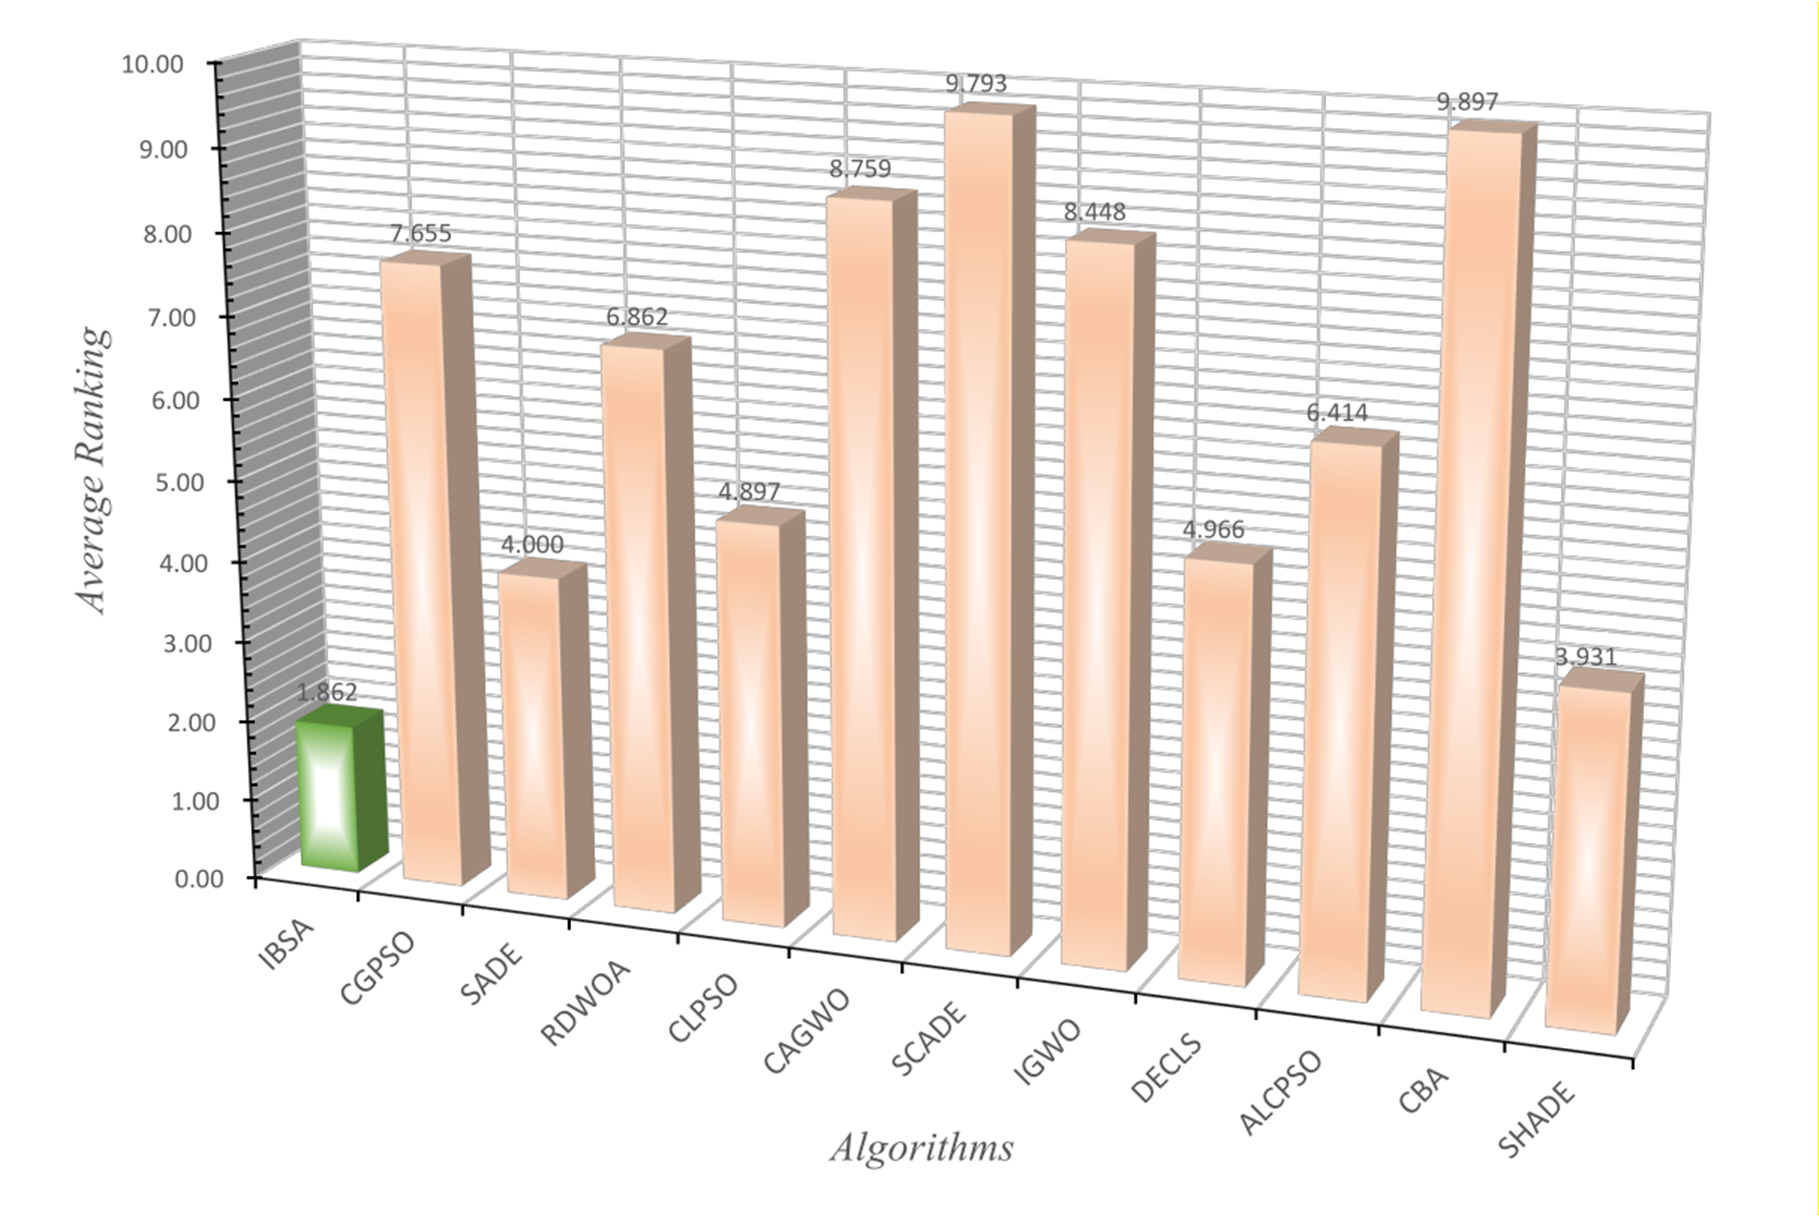
\includegraphics[width=\textwidth]{figures/fig7_friedman_ranking_advanced.png}
  \caption{Average ranking of IBSA and advance MAs.}
  \label{fig:friedman_ranking_advanced}
\end{figure}



In observing the performance of IBSA across a range of test functions, we are able to identify several notable strengths, as illustrated in Fig. 8. In single-modal functions, such as F1, we may observe that despite IBSA's convergence speed being somewhat slower than that of SHADE, both do obtain the same optimal solution, highlighting IBSA's competitive ability.

When considering multi-modal function F6, the convergence speed and solution accuracy of IBSA aligns with that of peers CLPSO and DECLS. Notably, in hybrid functions, namely F11, F13, F14, F15, and F19, IBSA's exceptional performance is evident as it maintains the top rank. Even though the convergence speed might be marginally slower than some algorithms, it's important to keep in mind that solution quality should take precedence over convergence speed.

In dealing with composition functions such as F23, F27, and F29, IBSA's stellar performance is evident from the convergence image, as it obtains a far superior solution compared to its counterparts. Notably, in the function F29, IBSA's performance is on par with SCADE.

Further, the box plot, situated next to the convergence curve, offers insight into the impressive robustness of the proposed IBSA. It displays minimal fluctuation rate and maintains the smallest fitness value over 30 runs, in comparison to the competitor algorithms. This detailed comparison effectively underscores the formidable capability of the IBSA algorithm.

\begin{figure}[htbp]
  \centering
  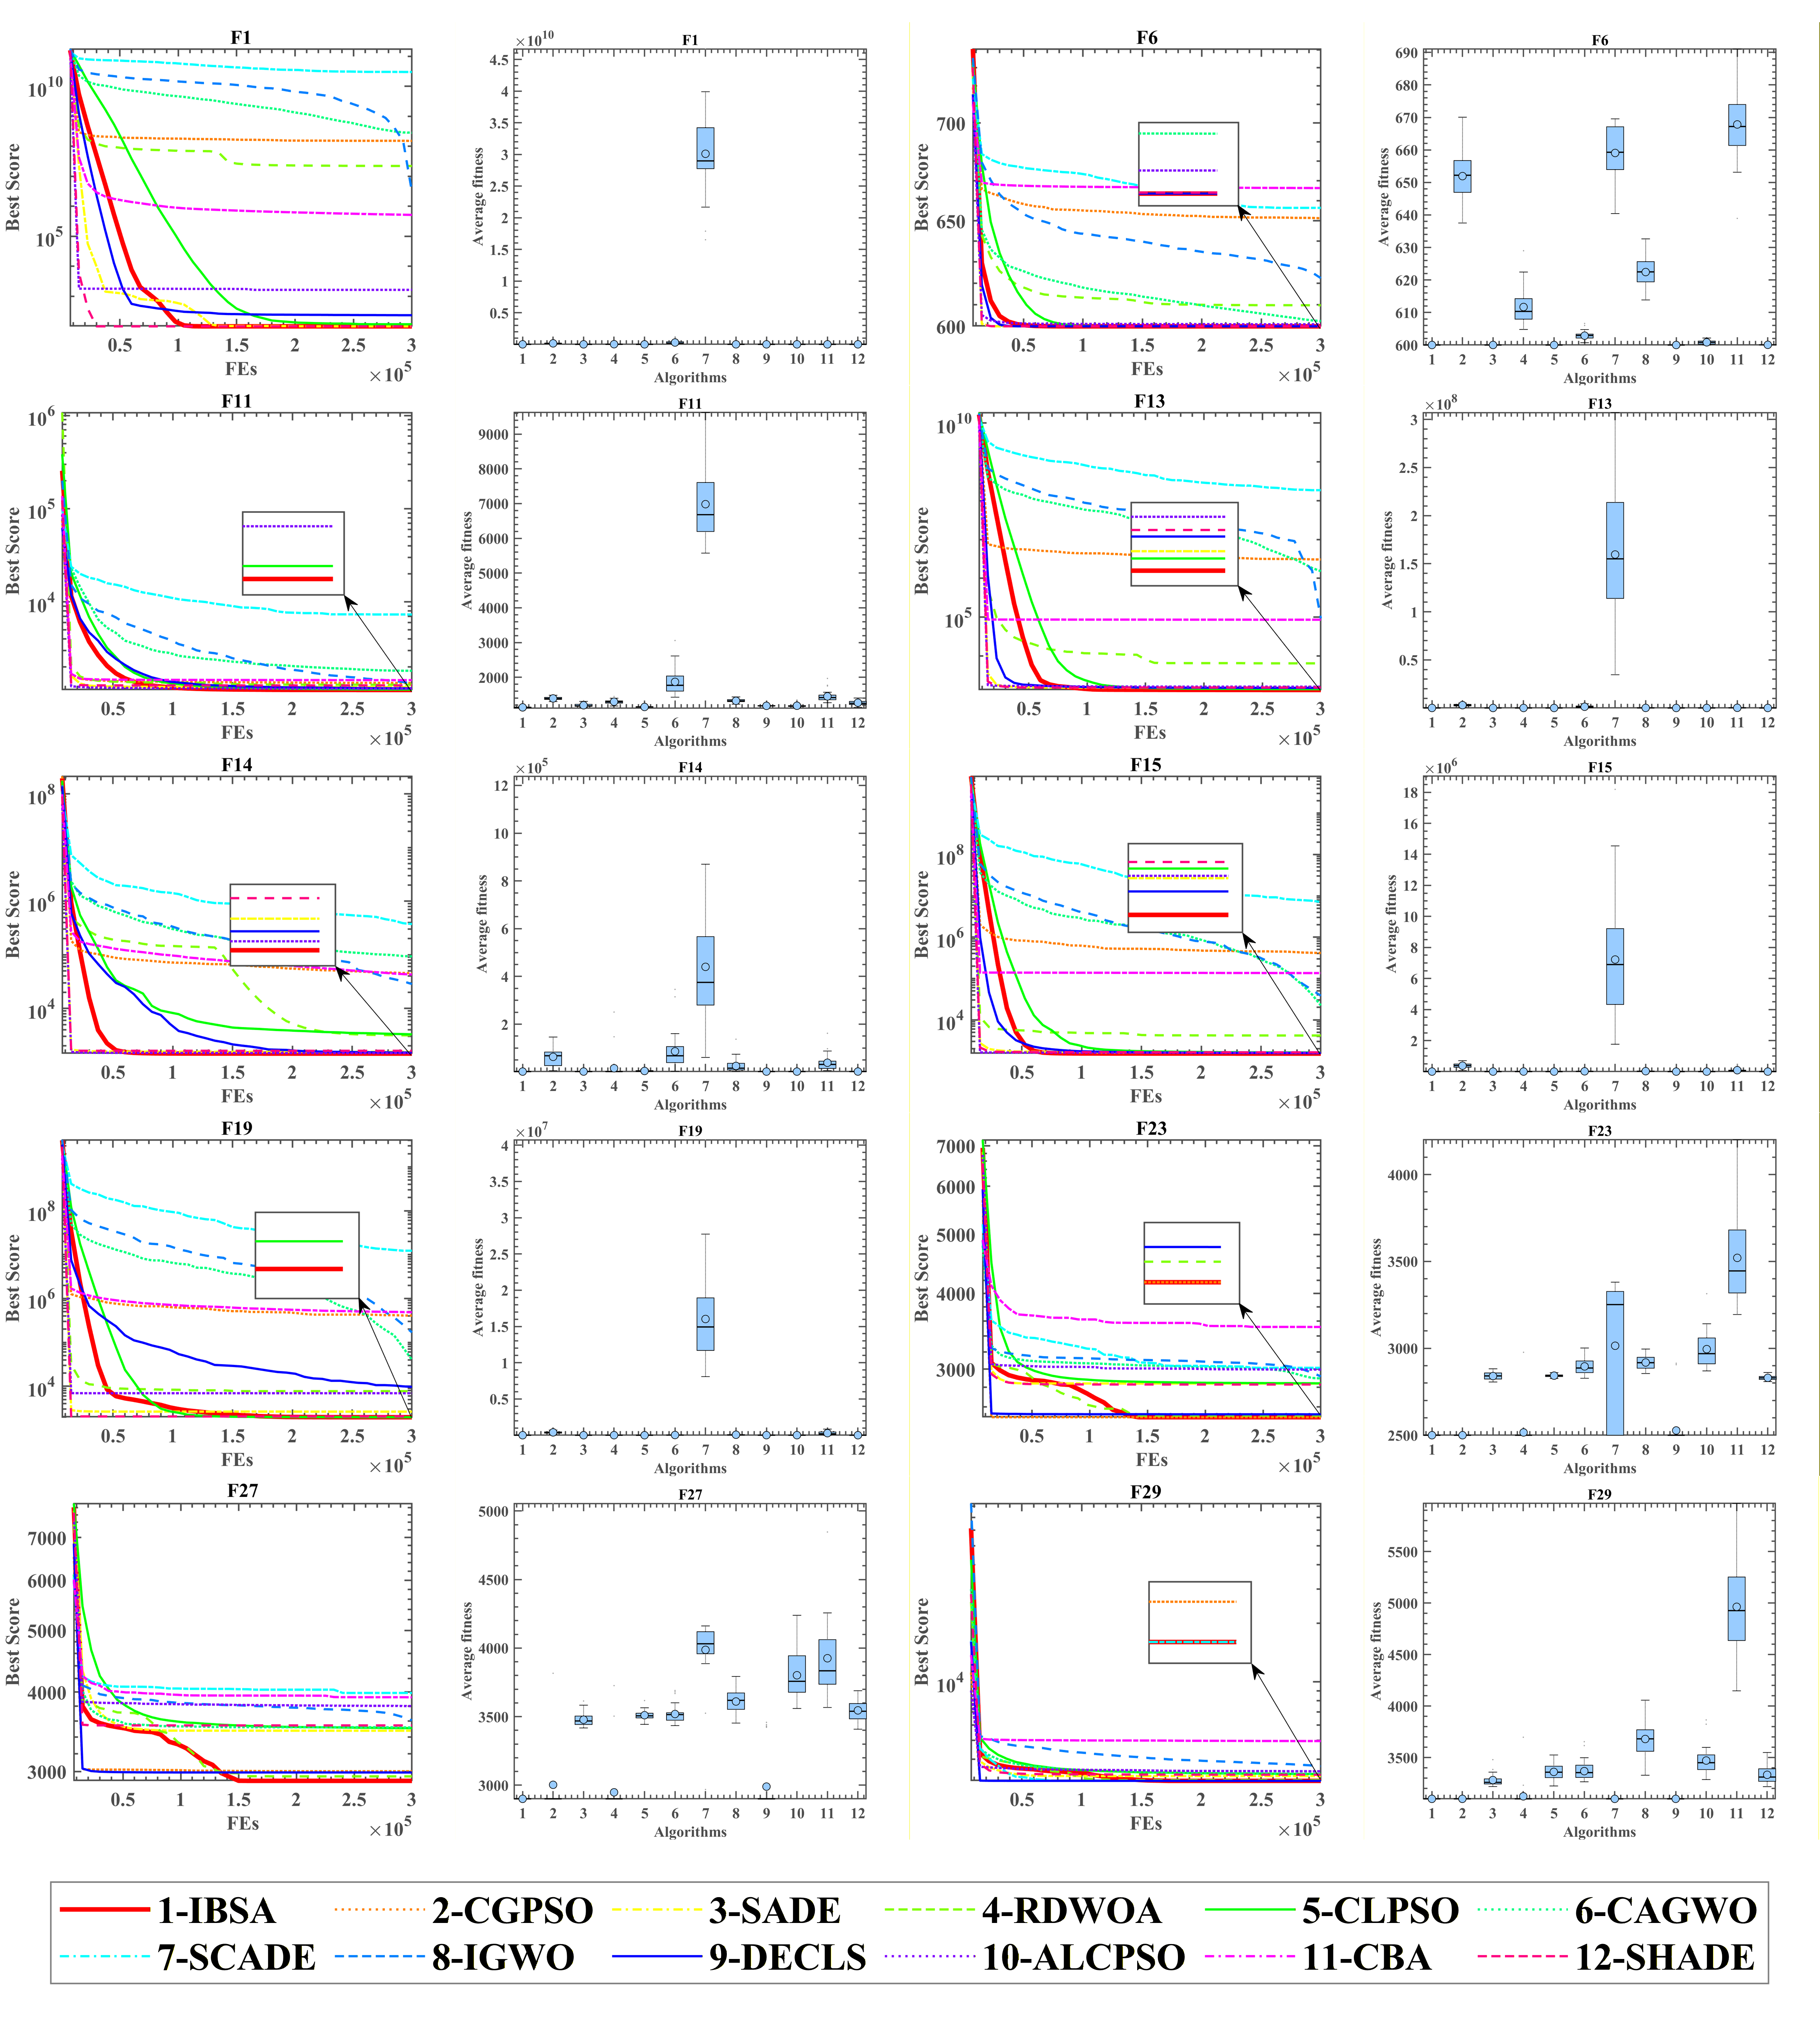
\includegraphics[width=\textwidth]{figures/fig8_convergence_advanced_MAs.png}
  \caption{Convergence curves and box plots of the IBSA and other advance MAs on 10 functions.}
  \label{fig:convergence_advanced_MAs}
\end{figure}




\section{ bIBSA for feature selection}

In this section, we touch upon the transformation [71] that has been applied to establish the binary version of IBSA, referred to as bIBSA. This version is set to be used to handle real-life engineering problems, more specifically, feature selection.

For our study, we selected 12 datasets from the publically available UCI dataset [93]. These datasets vary in dimensions, with the smallest dataset being 326 dimensions and the largest being 12,601. Out of these 12 datasets, nine have dimensions exceeding 5,000, and two have dimensions above 2,000. Only the penglung dataset, with a dimension count of 326, fell below these numbers.

These datasets, all hailing from the medical field, span a range of 2 to 7 classes and encompass various types and degrees of cancers and other diseases, each with distinct sample sizes, features, and class labels. It's essential to note that our study's central focus is to validate the performance of the proposed bIBSA in the binary problem domain. For a more detailed breakdown, Table 6 further elaborates on the specifics of these datasets.

As per the intricate details divulged in Table 6, it's evident that the datasets employed span a diverse range of medical conditions, including brain tumors, CNS, colon cancer, leukemia, lung cancer, and prostate tumors. The breadth of these conditions allows us to assess the robustness of bIBSA across various health domains.

Furthermore, the sheer diversity in feature numbers, ranging from 326 to 12,601, presents a unique opportunity to evaluate the algorithm's performance with both lower-dimensional and higher-dimensional data. This aids in gaining insight into the algorithm's handle on different feature spaces.

It's noteworthy to highlight that some datasets incorporate multiple classes, granting the ability to assess the proficiency of the algorithm in managing multi-class classification problems.

\begin{tabular}{|p{1.0in}|p{1.0in}|p{1.0in}|p{1.0in}|} \hline 
\multicolumn{4}{|p{1in}|}{\textbf{Table }6\textbf{.} Description of the datasets used} \\ \hline 
Dataset & Samples & Features & Classes \\ \hline 
Brain\_Tumor1 & 90 & 5920 & 5 \\ \hline 
Brain\_Tumor2 & 50 & 10367 & 4 \\ \hline 
CNS & 60 & 7130 & 2 \\ \hline 
Colon & 62 & 2001 & 2 \\ \hline 
DLBCL & 77 & 5470 & 4 \\ \hline 
Leukemia & 72 & 7131 & 2 \\ \hline 
Leukemia1 & 72 & 5328 & 5 \\ \hline 
Leukemia2 & 72 & 11225 & 3 \\ \hline 
Lung\_Cancer & 203 & 12601 & 3 \\ \hline 
penglung & 73 & 326 & 7 \\ \hline 
Prostate\_Tumor & 102 & 10509 & 2 \\ \hline 
SRBCT & 83 & 2390 & 4 \\ \hline 
\end{tabular}



Performance evaluation of IBSA involved comparing it with eight diverse algorithms, each holding unique parameter configurations as detailed in Table 7. Standardized parameters, such as dimensionality $(D)$ which represents the count of attributes within individual datasets, were effectively used across all evaluations. Additionally, the population size $(N)$ was set consistently at 20 for all the algorithms being compared.

In our pursuit of a fair evaluation of bIBSA's effectiveness in Feature Selection (FS), we deployed a meticulous 10-fold cross-validation technique [94]. This method partitions the dataset into ten equally-sized subsets, setting aside one as a test portion while utilizing the remaining nine as training segments over numerous iterations.

We conducted these comparative experiments within the MATLAB R2018a operation environment to maintain identical conditions throughout the testing processes.

\begin{tabular}{|p{1.1in}|p{2.8in}|} \hline 
\multicolumn{2}{|p{1in}|}{\textbf{Table }7\textbf{.} Setup of control parameter} \\ \hline 
Algorithm & Other parameters \\ \hline 
BMFO & $a=2;b=1$\textit{} \\ \hline 
BGWO & $a=\left[0,2\right]$\textit{} \\ \hline 
BGSA & $wMax\ =\ 20;\ wMin\ =\ 1e-10\ $\textit{} \\ \hline 
BPSO & $Max=0.9;\ Min=0.4\ $\textit{} \\ \hline 
BALO & $None$\textit{} \\ \hline 
BBA & $a=0.5;\ r=0.5$\textit{} \\ \hline 
BSSA & $a=2$\textit{} \\ \hline 
BWOA & $a\ =\ \left[0,2\right]$ \\ \hline 
\end{tabular}


\paragraph{ Evaluation metrics for bIBSA performance}

In this section, to effectively measure the performance of bIBSA in addressing feature selection challenges across various datasets, we've made use of specific evaluation metrics. These metrics allow us to assess the algorithm's performance in precise domains. Several crucial criteria, detailed in [95], were selected for this purpose which include average fitness, classification error rate, the average number of selected features by the optimizer, and average runtime. Together, these metrics provide a holistic understanding of bIBSA's performance in handling feature selection tasks across a range of datasets.

\begin{enumerate}
\item  \textbf{Average Fitness:}
\end{enumerate}

The average fitness value represents the overall fitness of bIBSA over $L$ independent runs on each dataset. It's calculated as shown in Eq. \eqref{GrindEQ__25_}.

\begin{tabular}{|p{0.4in}|p{2.9in}|p{0.5in}|} \hline 
 & $Fitness\mathrm{=\ }\frac{1}{L}\int^L_{i=1}{fitness\left(i\right)}$ & (25) \\ \hline 
\end{tabular}

Here $L$ denotes total runs of bIBSA, $Fitness$ is the average fitness value across $L$ runs, and $fitness\left(i\right)$ is the fitness value obtained from the $i$th run.

\begin{enumerate}
\item  \textbf{Average Classification Error Rate:}
\end{enumerate}

The classification accuracy of bIBSA was assessed by calculating the average classification error rate over $L$ runs, as shown in Eq. \eqref{GrindEQ__26_}.

\begin{tabular}{|p{0.4in}|p{2.9in}|p{0.5in}|} \hline 
 & $Error=\ \frac{1}{L}\int^L_{i=1}{\left(1-Accuracy\left(i\right)\right)\ }$ & (26) \\ \hline 
\end{tabular}

Here $L$ is the total runs, $Error$ is the average classification error rate, and $Accuracy\left(i\right)$ refers to the classification accuracy from the $ith$ run.

\begin{enumerate}
\item  \textbf{Average Number of Features Selected:}
\end{enumerate}

The average count of features picked by bIBSA across $L$ runs was calculated to understand feature selection tendencies of the algorithm, represented in Eq. \eqref{GrindEQ__27_}.

\begin{tabular}{|p{0.4in}|p{2.9in}|p{0.5in}|} \hline 
 & $Features\_num\mathrm{=\ }\frac{1}{L}\int^L_{i=1}{Size\left(i\right)}$ & (27) \\ \hline 
\end{tabular}

Here $Features\_num$ denotes average number of features selected, $Size\left(i\right)$ shows the number of features selected in the $ith$  run, and $L$ is the total runs.

\begin{enumerate}
\item  \textbf{Average Run-time:}
\end{enumerate}

The computational efficiency of bIBSA was evaluated by calculating its average run-time over $L$ runs as expressed in Eq. \eqref{GrindEQ__28_}.

\begin{tabular}{|p{0.4in}|p{2.9in}|p{0.5in}|} \hline 
 & $Time=\ \frac{1}{L}\int^L_{i=1}{Runtime\left(i\right)}$ & (28) \\ \hline 
\end{tabular}

Here $Time$ denotes average run-time for $L$  runs and $Runtime\left(i\right)$ is the time taken by bIBSA in the $i$th run.


\paragraph{ Experimental results and analysis of bIBSA}

In this section, the efficacy of bIBSA in Feature Selection is scrutinized through a comprehensive comparative analysis, pitting it against eight prominent optimization techniques---BMFO [96], BGWO [97], BGSA [98], BPSO [99], Binary Ant Lion Optimization (BALO) [100], Binary Bat Algorithm (BBA) [101], Binary Salp Swarm Algorithm (BSSA) [102], and BWOA [103]. This evaluation is conducted across a diverse set of 12 UCI datasets [93], examining a host of performance metrics including average fitness value, average number of features selected, average run-time, and average accuracy rate.

The assessment unfolded over 50 iterations executed using a 10-fold cross-validation [94] on each dataset. Detailed results for average fitness value, feature count, run-time, and error rate are diligently presented in Tables 8 to 11. The objective of this stringent evaluation was to assess the accuracy and robustness of bIBSA in identifying pertinent features from datasets of various dimensions.

Feature Selection performs a pivotal role in machine learning applications, immensely affecting the accuracy of predictive models and computational efficiency. This comprehensive investigation aims to provide an extensive evaluation of bIBSA's performance in Feature Selection, casting light on its strengths and possible limitations when compared against existing algorithms.

The comparative results in Table 8 reveal that the proposed bIBSA achieved the best fitness outcomes across all 12 datasets. Aside from a slightly larger Std when evaluating the Brain\_Tumor1, CNS, leukemia1, and penglung datasets compared to BPSO, overall, the results of bIBSA displayed significant efficacy. Against BWOA, a prominent method, bIBSA also exhibited comparatively larger Std results. Moreover, when considering the SRBCT dataset, bIBSA's performance matches BWOA in terms of fitness, but bIBSA significantly surpasses BWOA in terms of Std.

This evidence indicates that the proposed bIBSA showcases robust optimization performance when compared with traditional binary optimizers. This is a key finding, demonstrating the considerable potential of bIBSA in the realm of binary optimization and considerably broadening the implications for practical application.

\begin{tabular}{|p{0.6in}|p{0.3in}|p{0.4in}|p{0.4in}|p{0.4in}|p{0.4in}|p{0.4in}|p{0.4in}|p{0.4in}|p{0.4in}|p{0.4in}|} \hline 
\multicolumn{10}{|p{1in}|}{\textbf{Table }8\textbf{. }Comparison between bIBSA and other algorithms on average fitness values\textbf{}} & \textbf{} \\ \hline 
\textbf{Function} & \textbf{Metric} & \textbf{bIBSA} & \textbf{BMFO} & \textbf{BGWO} & \textbf{BGSA} & \textbf{BPSO} & \textbf{BALO} & \textbf{BBA} & \textbf{BSSA} & \textbf{BWOA} \\ \hline 
\textbf{Brain\_Tumor1} & Avg & \textbf{2.052E-02} & 2.430E-02 & 4.931E-02 & 8.643E-02 & 1.063E-01 & 8.556E-02 & 1.212E-01 & 7.872E-02 & 2.349E-02 \\ \hline 
\textbf{} & Std & 2.203E-02\textbf{} & 3.912E-02 & 3.522E-02 & 3.974E-02 & \textbf{2.064E-02} & 2.483E-02 & 3.954E-02 & 4.722E-02 & 4.266E-02 \\ \hline 
\textbf{Brain\_Tumor2} & Avg & \textbf{4.823E-06} & 2.122E-04 & 5.689E-03 & 2.280E-02 & 2.382E-02 & 2.364E-02 & 2.066E-01 & 2.446E-02 & 1.206E-05 \\ \hline 
\textbf{} & Std & \textbf{2.330E-06} & 2.582E-04 & 1.044E-01 & 7.896E-02 & 1.477E-01 & 1.150E-01 & 1.311E-01 & 5.302E-02 & 3.372E-06 \\ \hline 
\textbf{CNS} & Avg & \textbf{7.014E-06} & 6.979E-04 & 5.965E-03 & 2.276E-02 & 2.448E-02 & 2.373E-02 & 1.802E-01 & 1.755E-01 & 1.403E-05 \\ \hline 
\textbf{} & Std & 8.902E-06\textbf{} & 1.325E-03 & 6.219E-02 & 1.088E-01 & 7.638E-02 & 7.909E-02 & 1.556E-01 & 1.250E-01 & \textbf{7.539E-06} \\ \hline 
\textbf{Colon} & Avg & \textbf{2.500E-05} & 2.125E-04 & 4.188E-03 & 1.663E-01 & 1.805E-01 & 1.686E-01 & 1.737E-01 & 1.646E-01 & 6.250E-05 \\ \hline 
\textbf{} & Std & \textbf{1.687E-05} & 1.482E-04 & 1.335E-01 & 1.297E-01 & 1.100E-01 & 1.455E-01 & 1.536E-01 & 1.061E-01 & 3.344E-05 \\ \hline 
\textbf{DLBCL} & Avg & \textbf{9.142E-06} & 6.400E-05\textbf{} & 5.262E-03 & 2.146E-02 & 2.319E-02 & 2.296E-02 & 1.917E-02 & 2.344E-02 & 1.829E-05 \\ \hline 
\textbf{} & Std & \textbf{2.891E-06} & 7.710E-05\textbf{} & 4.289E-02 & 4.294E-02 & 2.662E-04 & 4.302E-02 & 3.560E-03 & 3.527E-02 & 1.380E-05 \\ \hline 
\textbf{Leukemia} & Avg & \textbf{7.013E-06} & 1.017E-04 & 5.354E-03 & 2.186E-02 & 2.347E-02 & 2.301E-02 & 1.823E-02 & 1.911E-02 & \textbf{7.013E-06} \\ \hline 
\textbf{} & Std & \textbf{8.929E-22} & 9.471E-05 & 2.067E-04 & 2.406E-04 & 2.343E-04 & 2.681E-04 & 3.676E-02 & 9.043E-03 & 3.621E-06 \\ \hline 
\textbf{Leukemia1} & Avg & \textbf{1.877E-05} & 2.394E-04 & 5.275E-03 & 2.134E-02 & 2.311E-02 & 2.292E-02 & 2.019E-02 & 9.724E-03 & 2.816E-05 \\ \hline 
\textbf{} & Std & 1.867E-05\textbf{} & 2.124E-04 & 3.119E-04 & 5.216E-04 & 3.777E-04 & 2.599E-04 & 2.134E-03 & 1.080E-02 & \textbf{1.033E-05} \\ \hline 
\textbf{Leukemia2} & Avg & \textbf{8.909E-06} & 1.180E-04\textbf{} & 5.405E-03 & 2.251E-02 & 2.373E-02\textbf{} & 2.336E-02 & 2.081E-02 & 2.419E-02 & 1.336E-05 \\ \hline 
\textbf{} & Std & \textbf{1.878E-06} & 5.962E-05\textbf{} & 2.407E-04 & 5.007E-02 & 4.290E-02\textbf{} & 5.391E-02 & 5.834E-02 & 5.991E-02 & 2.817E-06 \\ \hline 
\textbf{Lung\_Cancer} & Avg & \textbf{1.011E-02} & 1.522E-02 & 2.527E-02 & 4.133E-02 & 6.163E-02\textbf{} & 4.298E-02 & 4.256E-02 & 4.467E-02 & 1.923E-02 \\ \hline 
\textbf{} & Std & \textbf{1.241E-04} & 5.213E-04 & 2.053E-02 & 2.260E-02 & 3.230E-02\textbf{} & 2.458E-02 & 3.355E-02 & 2.616E-02 & 1.430E-02 \\ \hline 
\textbf{penglung} & Avg & \textbf{3.077E-04} & 6.154E-04\textbf{} & 1.308E-03\textbf{} & 1.139E-02 & 1.877E-02 & 1.731E-02 & 2.054E-02\textbf{} & 2.100E-02 & 4.615E-04 \\ \hline 
\textbf{} & Std & 3.512E-04 & 6.405E-04\textbf{} & 7.460E-04\textbf{} & 5.087E-02 & 5.491E-02 & 8.551E-02 & 7.809E-02\textbf{} & 1.063E-01 & \textbf{3.417E-04} \\ \hline 
\textbf{Prostate\_Tumor} & Avg & \textbf{7.137E-06} & 4.972E-04 & 6.266E-03 & 7.041E-02 & 6.709E-02\textbf{} & 2.402E-02 & 1.154E-01\textbf{} & 5.657E-02 & 1.665E-05 \\ \hline 
\textbf{} & Std & \textbf{3.327E-06} & 2.995E-02 & 4.585E-02 & 8.336E-02 & 8.952E-02\textbf{} & 6.644E-02 & 7.655E-02\textbf{} & 4.742E-02 & 2.427E-05 \\ \hline 
\textbf{SRBCT} & Avg & \textbf{6.499E-05} & 3.900E-04 & 4.159E-03 & 1.945E-02 & 2.213E-02\textbf{} & 2.170E-02 & 2.049E-02\textbf{} & 1.582E-03 & \textbf{6.499E-05} \\ \hline 
\textbf{} & Std & \textbf{3.689E-05} & 3.553E-04 & 2.628E-04 & 3.768E-02 & 5.694E-04\textbf{} & 6.278E-04 & 4.689E-02\textbf{} & 7.074E-02 & 8.312E-05 \\ \hline 
\end{tabular}



Table 9 reveals the average feature selection from 30 runs on a single dataset. A careful look at the results, especially those highlighted in bold, underscores the strong performance of our proposed solution, bIBSA, across different datasets. Remarkably, bIBSA selected the fewest features on average across all 12 datasets, demonstrating its strong optimization ability consistent with global under continuous optimization problems.

However, we do observe slightly larger fluctuations with the datasets Brain\_Tumor1, CNS, leukemia1, and Lung\_Cancer, judging by the Std values presented in the table. It's important to note, though, that a bit more fluctuation with more selected features does not necessarily imply an ineffective optimizer, given that the number of features selected and accuracy are the key indicators of a feature selection optimizer's effectiveness.

With reference to Table 10, which provides error rates for each feature selection method, the optimal optimizer should choose the fewest feature numbers in the dataset while maintaining the lowest error rate. Given that error occurrence is almost unavoidable, it's crucial to minimize the error rate as far as possible.

From the results, it's evident that bIBSA performs exceptionally well when compared with its peers. Although its Std value is slightly larger than that of BWOA, both of them recorded the lowest error rates. When considered across all 12 datasets, bIBSA's robustness is significantly evident.

\begin{tabular}{|p{0.6in}|p{0.3in}|p{0.4in}|p{0.4in}|p{0.4in}|p{0.4in}|p{0.4in}|p{0.4in}|p{0.4in}|p{0.4in}|p{0.4in}|} \hline 
\multicolumn{10}{|p{1in}|}{\textbf{Table }9\textbf{. }Comparison between bIBSA and other algorithms on average of selected features\textbf{}} & \textbf{} \\ \hline 
\textbf{Function} & \textbf{Metric} & \textbf{bIBSA} & \textbf{BMFO} & \textbf{BGWO} & \textbf{BGSA} & \textbf{BPSO} & \textbf{BALO} & \textbf{BBA} & \textbf{BSSA} & \textbf{BWOA} \\ \hline 
\textbf{Brain\_Tumor1} & Avg & \textbf{6.000E+01} & 2.545E+02 & 7.310E+02 & 2.602E+03 & 2.813E+03 & 2.767E+03 & 2.453E+03 & 1.874E+03 & 8.600E+01 \\ \hline 
\textbf{} & Std & 1.371E+02\textbf{} & 1.454E+02 & \textbf{2.522E+01} & 6.561E+01 & 5.817E+01 & 2.778E+01 & 2.132E+02 & 1.004E+03 & 4.333E+02 \\ \hline 
\textbf{Brain\_Tumor2} & Avg & \textbf{1.000E+00} & 4.400E+01 & 1.167E+03 & 4.684E+03 & 4.913E+03 & 4.877E+03 & 4.161E+03 & 5.072E+03 & 2.500E+00 \\ \hline 
\textbf{} & Std & \textbf{4.831E-01} & 5.353E+01 & 6.525E+01 & 6.727E+01 & 5.595E+01 & 4.249E+01 & 2.277E+02 & 2.095E+03 & 6.992E-01 \\ \hline 
\textbf{CNS} & Avg & \textbf{1.000E+00} & 9.950E+01 & 8.385E+02 & 3.227E+03 & 3.418E+03 & 3.345E+03 & 3.039E+03 & 3.467E+03 & 2.000E+00 \\ \hline 
\textbf{} & Std & 1.269E+00\textbf{} & 1.890E+02 & 3.116E+01 & 5.817E+01 & 6.487E+01 & 4.172E+01 & 1.688E+02 & 1.450E+03 & \textbf{1.075E+00} \\ \hline 
\textbf{Colon} & Avg & \textbf{1.000E+00} & 8.500E+00 & 1.575E+02 & 7.725E+02 & 8.855E+02 & 8.665E+02 & 8.055E+02 & 7.265E+02 & 2.500E+00 \\ \hline 
\textbf{} & Std & \textbf{6.750E-01} & 5.929E+00 & 1.204E+01 & 1.751E+01 & 1.960E+01 & 2.690E+01 & 6.086E+01 & 3.870E+02 & 1.338E+00 \\ \hline 
\textbf{DLBCL} & Avg & \textbf{1.000E+00} & 7.000E+00\textbf{} & 5.690E+02 & 2.344E+03 & 2.537E+03 & 2.511E+03 & 2.233E+03 & 2.523E+03 & 2.000E+00 \\ \hline 
\textbf{} & Std & \textbf{3.162E-01} & 8.433E+00\textbf{} & 2.858E+01 & 4.012E+01 & 2.912E+01 & 2.757E+01 & 1.303E+02 & 7.615E+02 & 1.509E+00 \\ \hline 
\textbf{Leukemia} & Avg & \textbf{1.000E+00} & 1.450E+01 & 7.635E+02 & 3.117E+03 & 3.347E+03 & 3.281E+03 & 2.919E+03 & 2.726E+03 & \textbf{1.000E+00} \\ \hline 
\textbf{} & Std & \textbf{0.000E+00} & 1.351E+01 & 2.948E+01 & 3.431E+01 & 3.340E+01 & 3.823E+01 & 1.787E+02 & 1.289E+03 & 5.164E-01 \\ \hline 
\textbf{Leukemia1} & Avg & \textbf{2.000E+00} & 2.550E+01 & 5.620E+02 & 2.274E+03 & 2.462E+03 & 2.442E+03 & 2.239E+03 & 1.036E+03 & 3.000E+00 \\ \hline 
\textbf{} & Std & 1.989E+00\textbf{} & 2.263E+01 & 3.323E+01 & 5.558E+01 & 4.024E+01 & 2.769E+01 & 9.345E+01 & 1.150E+03 & \textbf{1.101E+00} \\ \hline 
\textbf{Leukemia2} & Avg & \textbf{2.000E+00} & 2.650E+01\textbf{} & 1.214E+03 & 5.045E+03 & 5.326E+03\textbf{} & 5.245E+03 & 4.582E+03 & 5.430E+03 & 3.000E+00 \\ \hline 
\textbf{} & Std & \textbf{4.216E-01} & 1.338E+01\textbf{} & 5.404E+01 & 3.114E+01 & 3.767E+01\textbf{} & 3.395E+01 & 2.594E+02 & 1.867E+03 & 6.325E-01 \\ \hline 
\textbf{Lung\_Cancer} & Avg & \textbf{1.910E+02} & 1.285E+03 & 1.645E+03 & 5.898E+03 & 6.120E+03\textbf{} & 6.020E+03 & 5.202E+03 & 4.074E+03 & 2.505E+02 \\ \hline 
\textbf{} & Std & 9.347E+01\textbf{} & 5.636E+02 & 1.585E+02 & 1.231E+02 & \textbf{6.392E+01} & 7.051E+01 & 2.228E+02 & 2.964E+03 & 1.037E+02 \\ \hline 
\textbf{penglung} & Avg & \textbf{2.000E+00} & 4.000E+00\textbf{} & 8.500E+00\textbf{} & 7.400E+01 & 1.160E+02 & 1.090E+02 & 1.270E+02\textbf{} & 1.365E+02 & 3.000E+00 \\ \hline 
\textbf{} & Std & \textbf{1.838E+00} & 4.163E+00\textbf{} & 4.849E+00\textbf{} & 1.027E+01 & 6.430E+00 & 4.057E+00 & 1.274E+01\textbf{} & 6.083E+01 & 2.221E+00 \\ \hline 
\textbf{Prostate\_Tumor} & Avg & \textbf{1.500E+00} & 7.750E+01 & 1.298E+03 & 4.783E+03 & 5.041E+03\textbf{} & 4.975E+03 & 4.417E+03\textbf{} & 5.091E+03 & 3.500E+00 \\ \hline 
\textbf{} & Std & \textbf{6.992E-01} & 9.233E+01 & 6.168E+01 & 8.045E+01 & 6.521E+01\textbf{} & 6.365E+01 & 2.794E+02\textbf{} & 2.267E+03 & 5.100E+00 \\ \hline 
\textbf{SRBCT} & Avg & \textbf{3.000E+00} & 1.800E+01 & 1.920E+02 & 8.980E+02 & 1.022E+03\textbf{} & 1.002E+03 & 9.325E+02\textbf{} & 7.300E+01 & \textbf{3.000E+00} \\ \hline 
\textbf{} & Std & \textbf{1.703E+00} & 1.640E+01 & 1.213E+01 & 2.971E+01 & 2.628E+01\textbf{} & 2.898E+01 & 4.524E+01\textbf{} & 4.369E+02 & 3.837E+00 \\ \hline 
\end{tabular}



\begin{tabular}{|p{0.6in}|p{0.3in}|p{0.4in}|p{0.4in}|p{0.4in}|p{0.4in}|p{0.4in}|p{0.4in}|p{0.4in}|p{0.4in}|p{0.4in}|} \hline 
\multicolumn{10}{|p{1in}|}{\textbf{Table }10\textbf{. }Comparison between bIBSA and other algorithms on average of error rate\textbf{}} & \textbf{} \\ \hline 
\textbf{Function} & \textbf{Metric} & \textbf{bIBSA} & \textbf{BMFO} & \textbf{BGWO} & \textbf{BGSA} & \textbf{BPSO} & \textbf{BALO} & \textbf{BBA} & \textbf{BSSA} & \textbf{BWOA} \\ \hline 
\textbf{Brain\_Tumor1} & Avg & \textbf{2.083E-02} & 2.381E-02 & 4.555E-02 & 6.818E-02 & 8.696E-02 & 6.548E-02 & 1.739E-01 & 6.621E-02 & \textbf{2.083E-02} \\ \hline 
\textbf{} & Std & 2.520E-02\textbf{} & 4.204E-02 & 3.715E-02 & 4.150E-02 & \textbf{2.149E-02} & 2.634E-02 & 4.298E-02 & 5.820E-02 & 4.148E-02\textbf{} \\ \hline 
\textbf{Brain\_Tumor2} & Avg & \textbf{0.000E+00} & \textbf{0.000E+00} & \textbf{0.000E+00} & \textbf{0.000E+00} & \textbf{0.000E+00} & \textbf{0.000E+00} & 2.250E-01 & \textbf{0.000E+00} & \textbf{0.000E+00} \\ \hline 
\textbf{} & Std & \textbf{0.000E+00} & \textbf{0.000E+00} & 1.100E-01 & 8.315E-02 & 1.554E-01 & 1.209E-01 & 2.280E-01 & 5.271E-02 & \textbf{0.000E+00} \\ \hline 
\textbf{CNS} & Avg & \textbf{0.000E+00} & \textbf{0.000E+00} & \textbf{0.000E+00} & \textbf{0.000E+00} & \textbf{0.000E+00} & \textbf{0.000E+00} & 3.333E-01 & 1.667E-01 & \textbf{0.000E+00} \\ \hline 
\textbf{} & Std & \textbf{0.000E+00} & \textbf{0.000E+00} & 6.549E-02 & 1.145E-01 & 8.051E-02 & 8.328E-02 & 2.203E-01 & 1.315E-01 & \textbf{0.000E+00} \\ \hline 
\textbf{Colon} & Avg & \textbf{0.000E+00} & \textbf{0.000E+00} & \textbf{0.000E+00} & 1.548E-01 & 1.667E-01 & 1.548E-01 & 2.262E-01 & 1.548E-01 & \textbf{0.000E+00} \\ \hline 
\textbf{} & Std & \textbf{0.000E+00} & \textbf{0.000E+00} & 1.406E-01 & 1.365E-01 & 1.158E-01 & 1.528E-01 & 1.489E-01 & 1.042E-01 & \textbf{0.000E+00} \\ \hline 
\textbf{DLBCL} & Avg & \textbf{0.000E+00} & \textbf{0.000E+00} & \textbf{0.000E+00} & \textbf{0.000E+00} & \textbf{0.000E+00} & \textbf{0.000E+00} & \textbf{0.000E+00} & \textbf{0.000E+00} & \textbf{0.000E+00} \\ \hline 
\textbf{} & Std & \textbf{0.000E+00} & \textbf{0.000E+00} & 4.518E-02 & 4.518E-02 & \textbf{0.000E+00} & 4.518E-02 & 1.054E-01 & 3.953E-02 & \textbf{0.000E+00} \\ \hline 
\textbf{Leukemia} & Avg & \textbf{0.000E+00} & \textbf{0.000E+00} & \textbf{0.000E+00} & \textbf{0.000E+00} & \textbf{0.000E+00} & \textbf{0.000E+00} & \textbf{0.000E+00} & \textbf{0.000E+00} & \textbf{0.000E+00} \\ \hline 
\textbf{} & Std & \textbf{0.000E+00} & \textbf{0.000E+00} & \textbf{0.000E+00} & \textbf{0.000E+00} & \textbf{0.000E+00} & \textbf{0.000E+00} & 9.146E-02 & \textbf{0.000E+00} & \textbf{0.000E+00} \\ \hline 
\textbf{Leukemia1} & Avg & \textbf{0.000E+00} & \textbf{0.000E+00} & \textbf{0.000E+00} & \textbf{0.000E+00} & \textbf{0.000E+00} & \textbf{0.000E+00} & \textbf{0.000E+00} & \textbf{0.000E+00} & \textbf{0.000E+00} \\ \hline 
\textbf{} & Std & \textbf{0.000E+00} & \textbf{0.000E+00} & \textbf{0.000E+00} & \textbf{0.000E+00} & \textbf{0.000E+00} & \textbf{0.000E+00} & 7.313E-02 & \textbf{0.000E+00} & \textbf{0.000E+00} \\ \hline 
\textbf{Leukemia2} & Avg & \textbf{0.000E+00} & \textbf{0.000E+00} & \textbf{0.000E+00} & \textbf{0.000E+00} & \textbf{0.000E+00} & \textbf{0.000E+00} & \textbf{0.000E+00} & \textbf{0.000E+00} & \textbf{0.000E+00} \\ \hline 
\textbf{} & Std & \textbf{0.000E+00} & \textbf{0.000E+00} & \textbf{0.000E+00} & 5.271E-02 & 4.518E-02\textbf{} & 5.663E-02 & 6.227E-02 & 6.023E-02 & \textbf{0.000E+00} \\ \hline 
\textbf{Lung\_Cancer} & Avg & \textbf{0.000E+00} & \textbf{0.000E+00} & \textbf{0.000E+00} & \textbf{0.000E+00} & \textbf{0.000E+00} & \textbf{0.000E+00} & 9.524E-02 & 2.381E-02 & \textbf{0.000E+00} \\ \hline 
\textbf{} & Std & \textbf{0.000E+00} & \textbf{0.000E+00} & 2.165E-02 & 2.378E-02 & 3.410E-02\textbf{} & 2.588E-02 & 4.651E-02 & 2.646E-02 & 1.506E-02 \\ \hline 
\textbf{penglung} & Avg & \textbf{0.000E+00} & \textbf{0.000E+00} & \textbf{0.000E+00} & \textbf{0.000E+00} & \textbf{0.000E+00} & \textbf{0.000E+00} & 5.000E-02\textbf{} & \textbf{0.000E+00} & \textbf{0.000E+00} \\ \hline 
\textbf{} & Std & \textbf{0.000E+00} & \textbf{0.000E+00} & \textbf{0.000E+00} & 5.271E-02 & 5.795E-02 & 9.042E-02 & 9.350E-02\textbf{} & 1.084E-01 & \textbf{0.000E+00} \\ \hline 
\textbf{Prostate\_Tumor} & Avg & \textbf{0.000E+00} & \textbf{0.000E+00} & \textbf{0.000E+00} & 5.000E-02 & 4.546E-02\textbf{} & \textbf{0.000E+00} & 2.364E-01\textbf{} & 4.546E-02 & \textbf{0.000E+00} \\ \hline 
\textbf{} & Std & \textbf{0.000E+00} & 3.162E-02 & 4.831E-02 & 8.764E-02 & 9.431E-02\textbf{} & 6.992E-02 & 8.106E-02\textbf{} & 5.182E-02 & \textbf{0.000E+00} \\ \hline 
\textbf{SRBCT} & Avg & \textbf{0.000E+00} & \textbf{0.000E+00} & \textbf{0.000E+00} & \textbf{0.000E+00} & \textbf{0.000E+00} & \textbf{0.000E+00} & \textbf{0.000E+00} & \textbf{0.000E+00} & \textbf{0.000E+00} \\ \hline 
\textbf{} & Std & \textbf{0.000E+00} & \textbf{0.000E+00} & \textbf{0.000E+00} & 3.953E-02 & \textbf{0.000E+00} & \textbf{0.000E+00} & 9.982E-02\textbf{} & 7.027E-02 & \textbf{0.000E+00} \\ \hline 
\end{tabular}



Owing to the use of a v-shaped transformation function [71] and the efficient Elite Leading Mutation Strategy, our proposed bIBSA continues to hold a competitive edge in terms of execution time compared to the eight classical feature selection counterparts. Detailed data from Table 11 also corroborates this, revealing that bIBSA achieved the shortest run-time across all 12 datasets.

Although the Std for some datasets appears somewhat unstable, it is the Avg value statistic that is of primary importance. The Avg value results for bIBSA reflect clear advantages, including comparatively less time required to select the optimal features.

This translates to more efficiency in processing a variety of datasets and a significant reduction in computational resources. This is an aspect that offers immense potential value, particularly in a big-data context where efficient resource utilization is critical.

\begin{tabular}{|p{0.6in}|p{0.3in}|p{0.4in}|p{0.4in}|p{0.4in}|p{0.4in}|p{0.4in}|p{0.4in}|p{0.4in}|p{0.4in}|p{0.4in}|} \hline 
\multicolumn{10}{|p{1in}|}{\textbf{Table }11\textbf{. }Comparison between bIBSA and other algorithms on average of run time\textbf{}} & \textbf{} \\ \hline 
\textbf{Function} & \textbf{Metric} & \textbf{bIBSA} & \textbf{BMFO} & \textbf{BGWO} & \textbf{BGSA} & \textbf{BPSO} & \textbf{BALO} & \textbf{BBA} & \textbf{BSSA} & \textbf{BWOA} \\ \hline 
\textbf{Brain\_Tumor1} & Avg & \textbf{3.310E+00} & 4.635E+00 & 1.227E+01 & 1.017E+01 & 7.354E+00 & 7.104E+00 & 7.148E+00 & 7.056E+00 & 3.986E+00 \\ \hline 
\textbf{} & Std & \textbf{1.023E-01} & 2.885E-01 & 2.615E-01 & 3.163E-01 & 1.611E-01 & 1.768E-01 & 1.453E-01 & 3.080E-01 & 4.000E-01 \\ \hline 
\textbf{Brain\_Tumor2} & Avg & \textbf{1.680E+01} & 1.997E+01 & 6.234E+01 & 4.248E+01 & 2.345E+01 & 2.239E+01 & 2.375E+01 & 2.243E+01 & 2.005E+01 \\ \hline 
\textbf{} & Std & 1.110E+00\textbf{} & 1.289E+00 & 4.806E-01 & 2.262E+00 & 2.335E-01 & \textbf{1.458E-01} & 2.553E-01 & 2.120E-01 & 1.126E+00 \\ \hline 
\textbf{CNS} & Avg & \textbf{6.683E+00} & 7.217E+00 & 1.738E+01 & 1.289E+01 & 9.904E+00 & 9.625E+00 & 1.028E+01 & 9.382E+00 & 6.829E+00 \\ \hline 
\textbf{} & Std & 2.180E-01\textbf{} & 1.258E-01 & 2.528E-01 & \textbf{6.342E-02} & 6.381E-02 & 1.402E-01 & 1.513E-01 & 2.119E-01 & 1.564E-01 \\ \hline 
\textbf{Colon} & Avg & \textbf{1.139E+00} & 1.273E+00 & 3.952E+00 & 2.674E+00 & 1.640E+00 & 1.586E+00 & 1.737E+00 & 1.663E+00 & 1.220E+00 \\ \hline 
\textbf{} & Std & 6.370E-02\textbf{} & 5.286E-02 & 5.879E-02 & 2.756E-02 & \textbf{2.017E-02} & 4.013E-02 & 3.077E-02 & 3.126E-02 & 3.892E-02 \\ \hline 
\textbf{DLBCL} & Avg & \textbf{9.584E+00} & 9.900E+00\textbf{} & 2.810E+01 & 2.141E+01 & 1.513E+01 & 1.541E+01 & 1.579E+01 & 1.589E+01 & 1.011E+01 \\ \hline 
\textbf{} & Std & 8.610E-01\textbf{} & 6.400E-01\textbf{} & 4.706E-01 & \textbf{2.757E-01} & 1.501E+00 & 1.367E+00 & 1.389E+00 & 1.366E+00 & 7.260E-01 \\ \hline 
\textbf{Leukemia} & Avg & \textbf{1.741E+01} & 1.905E+01 & 5.189E+01 & 4.187E+01 & 2.817E+01 & 2.711E+01 & 2.816E+01 & 2.754E+01 & 1.912E+01 \\ \hline 
\textbf{} & Std & 7.162E-01\textbf{} & 6.216E-01 & \textbf{3.978E-01} & 7.265E-01 & 9.671E-01 & 7.486E-01 & 9.918E-01 & 8.984E-01 & 7.376E-01 \\ \hline 
\textbf{Leukemia1} & Avg & \textbf{5.541E+00} & 6.217E+00 & 1.286E+01 & 1.082E+01 & 9.149E+00 & 8.995E+00 & 9.726E+00 & 8.935E+00 & 6.263E+00 \\ \hline 
\textbf{} & Std & 2.057E-01\textbf{} & 1.377E-01 & 1.791E-01 & 1.041E-01 & \textbf{9.460E-02} & 1.002E-01 & 1.577E-01 & 1.779E-01 & 1.202E-01 \\ \hline 
\textbf{Leukemia2} & Avg & \textbf{2.529E+01} & 2.920E+01\textbf{} & 7.911E+01 & 7.198E+01 & 4.598E+01\textbf{} & 4.434E+01 & 4.580E+01 & 4.343E+01 & 3.246E+01 \\ \hline 
\textbf{} & Std & 1.987E+00 & 2.272E+00\textbf{} & \textbf{1.199E+00} & 6.624E+00 & 4.282E+00\textbf{} & 3.939E+00 & 4.115E+00 & 4.189E+00 & 2.176E+00 \\ \hline 
\textbf{Lung\_Cancer} & Avg & \textbf{4.652E+01} & 7.595E+01 & 1.860E+02 & 1.695E+02 & 1.442E+02\textbf{} & 1.422E+02 & 1.426E+02 & 1.323E+02 & 6.845E+01 \\ \hline 
\textbf{} & Std & 7.422E-01\textbf{} & 3.155E+00 & 1.524E+00 & \textbf{6.048E-01} & 2.031E+00\textbf{} & 1.812E+00 & 1.718E+00 & 1.995E+00 & 3.524E+00 \\ \hline 
\textbf{penglung} & Avg & \textbf{1.107E+00} & 1.109E+00\textbf{} & 1.711E+00\textbf{} & 1.418E+00 & 1.206E+00 & 1.177E+00 & 1.230E+00\textbf{} & 1.200E+00 & 1.175E+00 \\ \hline 
\textbf{} & Std & \textbf{4.834E-02} & 5.677E-02\textbf{} & 1.014E-01\textbf{} & 6.998E-02 & 6.841E-02 & 6.465E-02 & 8.204E-02\textbf{} & 6.072E-02 & 6.548E-02 \\ \hline 
\textbf{Prostate\_Tumor} & Avg & \textbf{3.198E+01} & 3.846E+01 & 8.591E+01 & 8.474E+01 & 6.095E+01\textbf{} & 5.924E+01 & 6.103E+01\textbf{} & 5.677E+01 & 3.595E+01 \\ \hline 
\textbf{} & Std & 3.282E+00\textbf{} & \textbf{2.825E+00} & 2.869E+00 & 8.037E+00 & 6.036E+00\textbf{} & 5.406E+00 & 5.675E+00\textbf{} & 4.931E+00 & 3.060E+00 \\ \hline 
\textbf{SRBCT} & Avg & \textbf{2.862E+00} & 3.092E+00 & 5.905E+00 & 4.782E+00 & 4.012E+00\textbf{} & 3.930E+00 & 4.288E+00\textbf{} & 3.915E+00 & 2.893E+00 \\ \hline 
\textbf{} & Std & 7.068E-02 & 7.428E-02 & 1.645E-01 & 7.003E-02 & 7.041E-02\textbf{} & 7.393E-02 & \textbf{4.384E-02} & 1.033E-01 & 4.968E-02\textbf{} \\ \hline 
\end{tabular}



To more effectively present the results attained by the eight feature selection optimizers, Fig. 9 provides the convergence curves corresponding to all 12 datasets. The graph clearly demonstrates that our proposed bIBSA consistently outperforms its peers in terms of fitness value and solution accuracy.

Most of the feature selection peers tend to converge to a higher fitness value quite early on, whereas our bIBSA significantly maintains and even improves its gained fitness value over time. This further highlights the advantages of incorporating the elite leading mutation strategy into the bIBSA algorithms.

Notably, while there is only a marginal advantage for bIBSA over BWOA on datasets such as CNS, leukemia1, penglung, and SRBCT, a detailed inspection of the plotted graph reveals superior results achieved by bIBSA. This strongly signifies the optimization capability of the elite leading mutation strategy implemented in bIBSA.

Validating bIBSA through both benchmark global optimization tests and real-life engineering problem feature selection further underscores the solution's optimization capability. Given its potential, it is plausible to anticipate the algorithm's application in future research directions such as image segmentation, road planning, and recommender systems.

\begin{figure}[htbp]
  \centering
  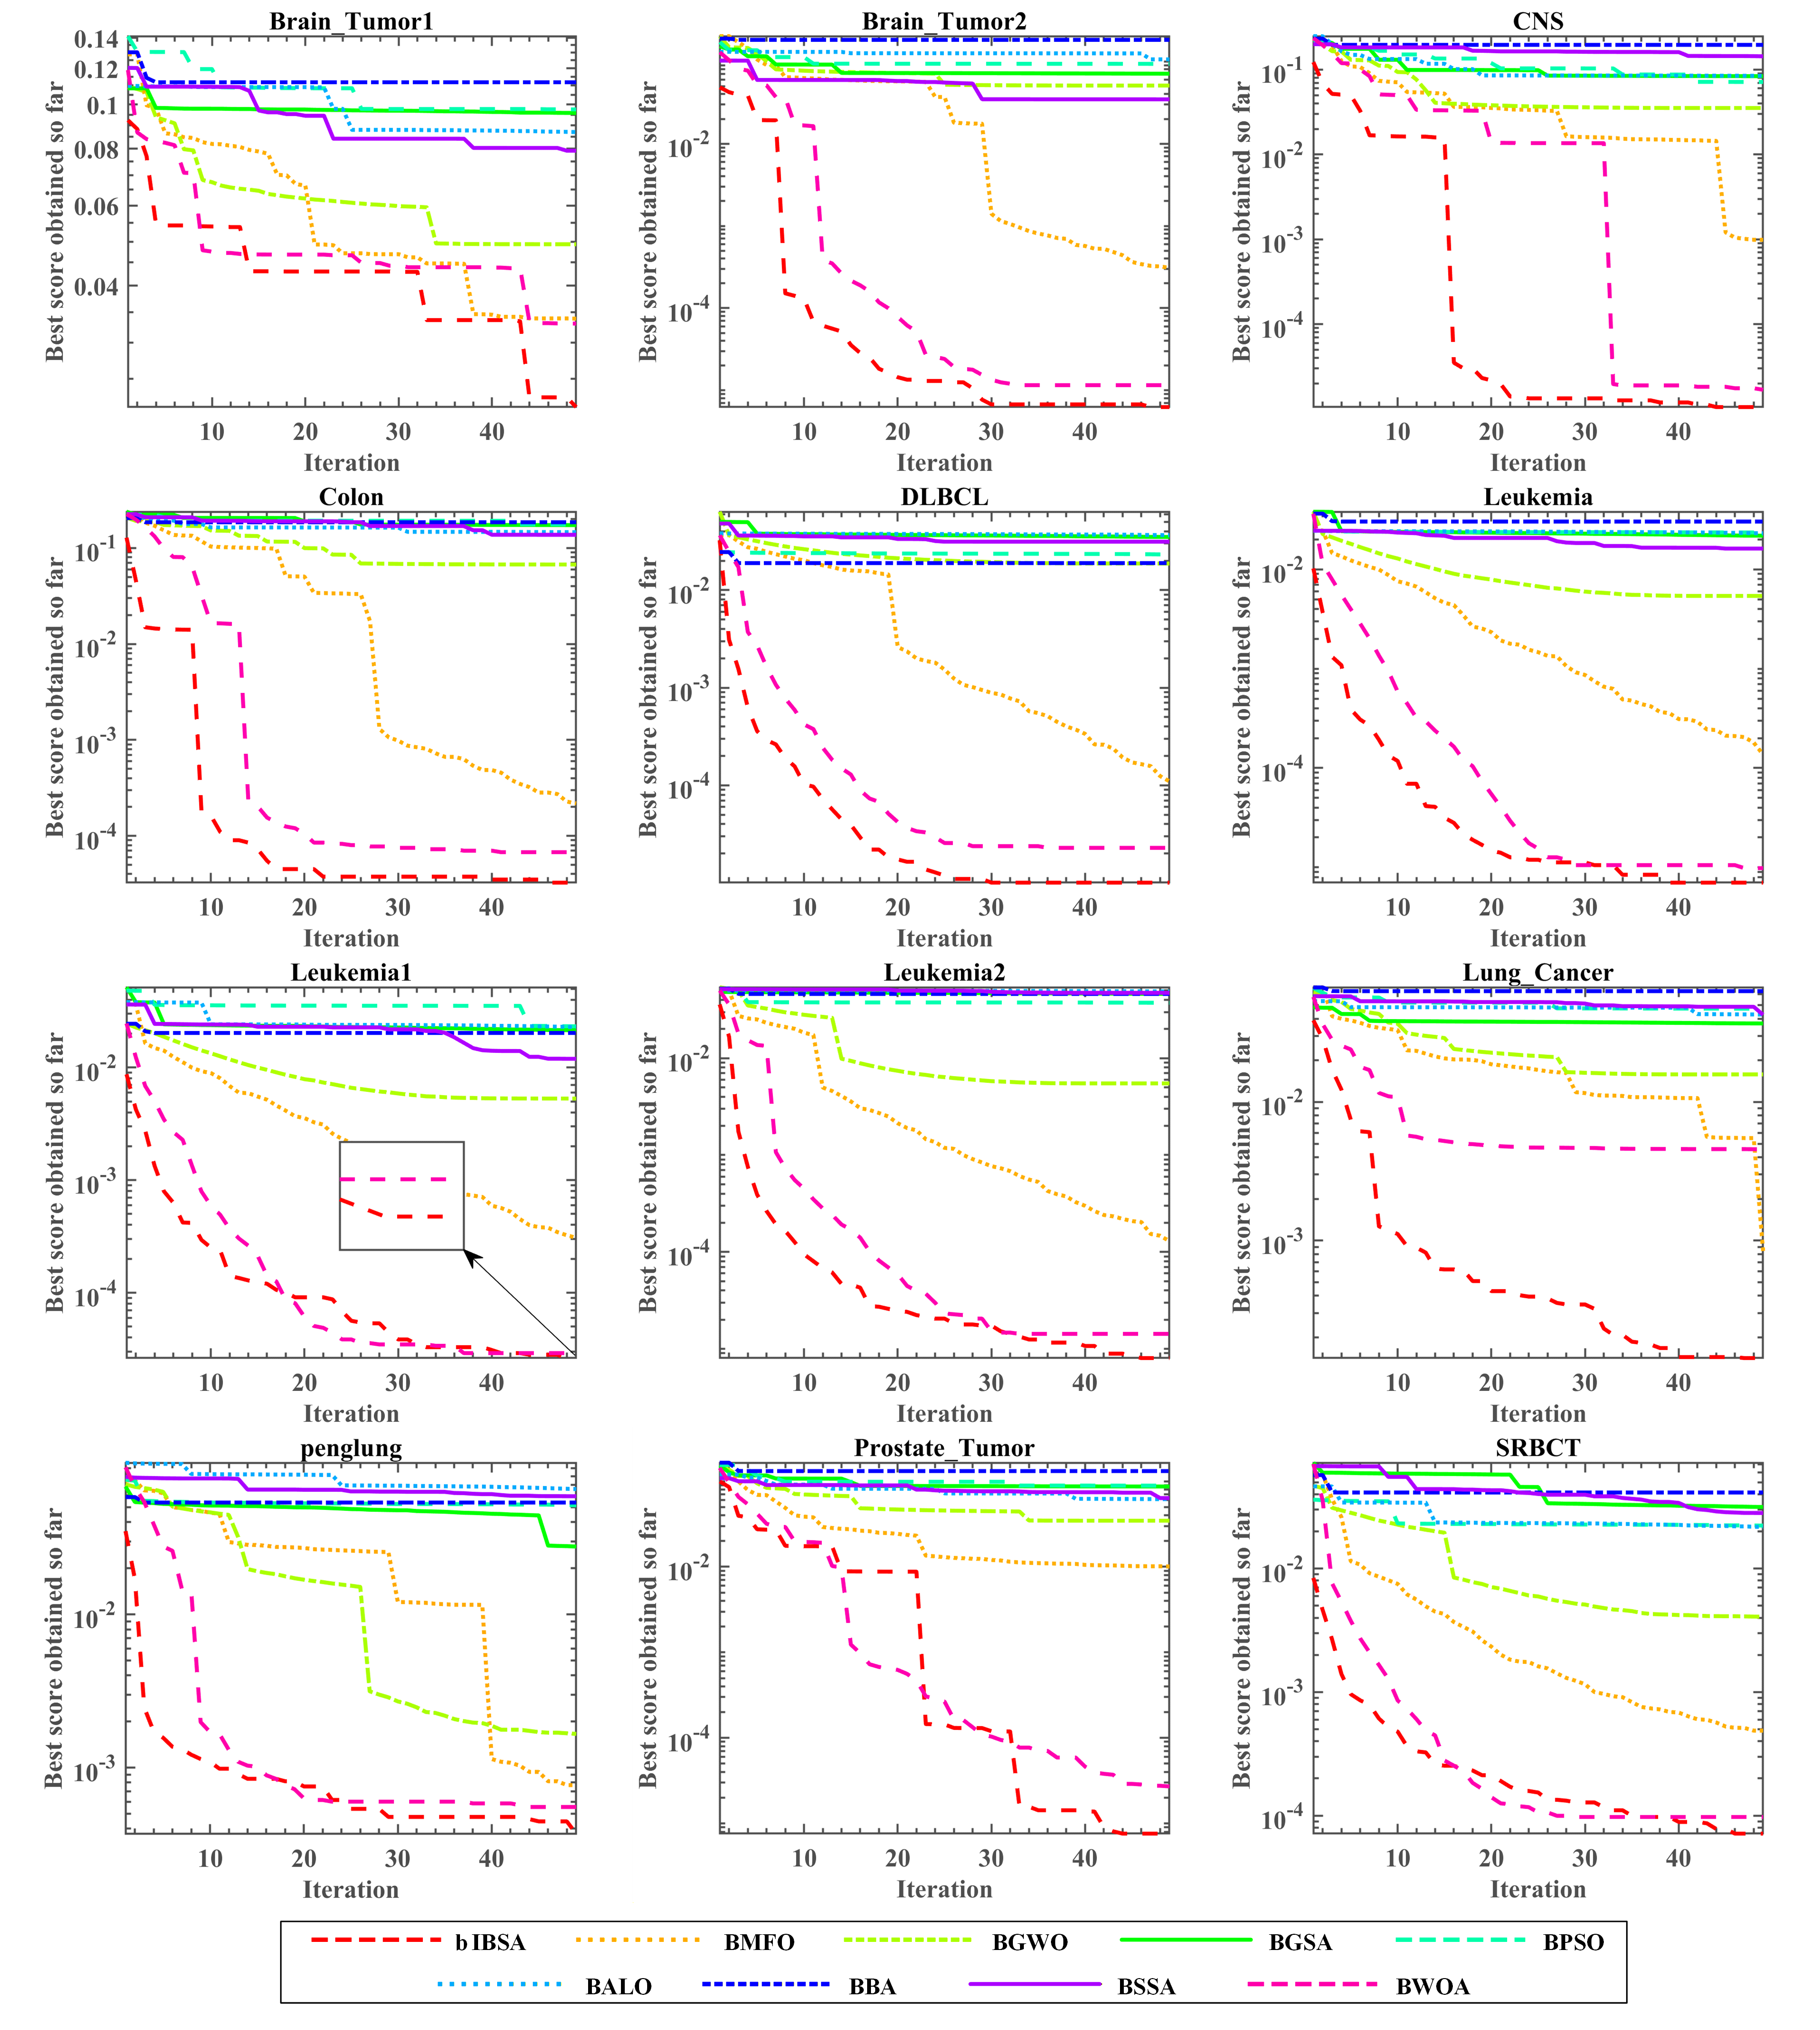
\includegraphics[width=\textwidth]{figures/fig9_convergence_feature_selection.png}
  \caption{Convergence curves of the bIBSA and other algorithms on 12 datasets.}
  \label{fig:convergence_feature_selection}
\end{figure}


\section{ Conclusion and future direction}

The primary aim of this research was to enhance the original BSA algorithm, particularly by mitigating its inherent randomness. Specifically, the random selection of historical populations and mutation strategies presented potential obstacles to predictable search direction and, consequently, to the quality improvement of later population generations. Especially given that the information inherent in the original BSA's historical populations and mutation strategies have proved to be proficient in contributing to the strong exploration ability of BSA. Therefore, this study notably focuses on modifying the original BSA to separate the elite individuals from the rest of the population, facilitating better utilization of the elite individuals' information for an improved optimal solution. Modifications include the selection processes between the historical populations and mutation operators. Additionally, to better implement the elite leading mutation strategy, a vector $m$ was proposed for the mutation operator during the global crossover phase, and a specific elite mutation operator was introduced to enhance the local exploitation of the elite individuals, ultimately improving solution accuracy. This modification led to a new strategy called the elite leading mutation strategy. Our comprehensive experimentation involved using the IEEE CEC 2017 suite, excluding function F2 due to the author's assertion of its instability. Impressive performance was evident as the proposed IBSA competed with a total of 23 peers, including 12 basic state-of-the-art algorithms and 11 advanced state-of-the-art algorithms. Following the benchmark global optimization testing of IBSA, we further explored its optimization capability in binary problem domains, using a v-shaped transformation function to convert the proposed IBSA to a binary version (bIBSA) and applying it to real-life engineering problem feature selection on 12 UCI public datasets. The results demonstrated bIBSA's superior performance over eight other feature selection optimizers in terms of the number and accuracy of features selected. Further value was evident in bIBSA's performance on high-dimensional datasets and in its competitive overall running time as compared to the eight classical optimizers. This means that using the proposed bIBSA algorithm for feature selection tasks promises to save significant computational resources.

Although this research paper provides substantial evidence for IBSA's robust capabilities in global optimization and feature selection within a 30-dimension framework, it is constrained by its scope. It warrants further investigation into higher dimensional spaces, such as 50 or 100 dimensions, to more comprehensively evaluate the powerful potential of IBSA. The application of the proposed IBSA algorithm has demonstrated impressive results in medical data feature selection, presenting a leap forward in the handling of high-dimensional datasets and streamlining data processing in healthcare settings. Looking ahead, there's a promising avenue for expanding the use of IBSA to tackle engineering challenges [104] and to refine machine learning methodologies [105], where its capabilities could lead to significant improvements in energy efficiency and parameter optimization. The insights gained from this study pave the way for future explorations that will unlock the untapped potentials of the BSA algorithm.

\noindent 
\section{Acknowledgments}

\noindent 
\section{Reference}

\noindent 

\noindent 

\noindent 1. Cao, L., et al., Decision-making optimization model for the targeted sustainable maintenance of a complex road network. Journal of Cleaner Production, 2024. 434: p. 139891.2. Gholamian, M.R., S.M.T. Fatemi Ghomi, and M. Ghazanfari, A hybrid intelligent system for multiobjective decision making problems. Computers \& Industrial Engineering, 2006. 51\eqref{GrindEQ__1_}: p. 26-43.3. Cai, Q., X. Guo, and S. Huang, A self-supervised learning model for graph clustering optimization problems. Knowledge-Based Systems, 2024. 290: p. 111549.4. Papadimitriou, C.H. and K. Steiglitz, Combinatorial optimization: algorithms and complexity. 1998: Courier Corporation.5. Luo, C., et al., NuSC: An Effective Local Search Algorithm for Solving the Set Covering Problem. IEEE Transactions on Cybernetics, 2024. 54\eqref{GrindEQ__3_}: p. 1403-1416.6. Cai, X., et al., The Collaborative Local Search Based on Dynamic-Constrained Decomposition With Grids for Combinatorial Multiobjective Optimization. IEEE Transactions on Cybernetics, 2021. 51\eqref{GrindEQ__5_}: p. 2639-2650.7. Ray, P., S.S. Reddy, and T. Banerjee, Various dimension reduction techniques for high dimensional data analysis: a review. Artificial Intelligence Review, 2021. 54\eqref{GrindEQ__5_}: p. 3473-3515.8. Rudin, C., et al., Machine Learning for the New York City Power Grid. IEEE Transactions on Pattern Analysis and Machine Intelligence, 2012. 34\eqref{GrindEQ__2_}: p. 328-345.9. Toaza, B. and D. Eszterg?r-Kiss, A review of metaheuristic algorithms for solving TSP-based scheduling optimization problems Image 1. Applied Soft Computing, 2023. 148: p. 110908.10. Anc\u{a}u, M., The optimization of printed circuit board manufacturing by improving the drilling process productivity. Computers \& Industrial Engineering, 2008. 55\eqref{GrindEQ__2_}: p. 279-294.11. Shendure, J., et al., DNA sequencing at 40: past, present and future. Nature, 2017. 550(7676): p. 345-353.12. Ferrell, W., et al., Horizontal collaboration: opportunities for improved logistics planning. International Journal of Production Research, 2020. 58\eqref{GrindEQ__14_}: p. 4267-4284.13. Wang, R., J. Yan, and X. Yang, Unsupervised Learning of Graph Matching With Mixture of Modes via Discrepancy Minimization. IEEE Transactions on Pattern Analysis and Machine Intelligence, 2023. 45\eqref{GrindEQ__8_}: p. 10500-10518.14. Ming-Syan, C., H. Jiawei, and P.S. Yu, Data mining: an overview from a database perspective. IEEE Transactions on Knowledge and Data Engineering, 1996. 8\eqref{GrindEQ__6_}: p. 866-883.15. Min, S., B. Lee, and S. Yoon, Deep learning in bioinformatics. Briefings in bioinformatics, 2017. 18\eqref{GrindEQ__5_}: p. 851-869.16. Cymerys, K. and M. Oszust, Attraction--Repulsion Optimization Algorithm for Global Optimization Problems. Swarm and Evolutionary Computation, 2024. 84: p. 101459.17. Zhang, T., et al., Correlated Differential Privacy: Feature Selection in Machine Learning. IEEE Transactions on Industrial Informatics, 2020. 16\eqref{GrindEQ__3_}: p. 2115-2124.18. Verleysen, M. and D. Fran?ois. The Curse of Dimensionality in Data Mining and Time Series Prediction. in Computational Intelligence and Bioinspired Systems. 2005. Berlin, Heidelberg: Springer Berlin Heidelberg.19. Luo, C., et al., Large-Scale Meta-Heuristic Feature Selection Based on BPSO Assisted Rough Hypercuboid Approach. IEEE Transactions on Neural Networks and Learning Systems, 2023. 34\eqref{GrindEQ__12_}: p. 10889-10903.20. Jha, K. and S. Saha, Incorporation of multimodal multiobjective optimization in designing a filter based feature selection technique. Applied Soft Computing, 2021. 98: p. 106823.21. S, K.P. and P.K. K, An embedded feature selection approach for depression classification using short text sequences. Applied Soft Computing, 2023. 147: p. 110828.22. Vommi, A.M. and T.K. Battula, A hybrid filter-wrapper feature selection using Fuzzy KNN based on Bonferroni mean for medical datasets classification: A COVID-19 case study. Expert Systems with Applications, 2023. 218: p. 119612.23. Al-Yaseen, W.L., A.K. Idrees, and F.H. Almasoudy, Wrapper feature selection method based differential evolution and extreme learning machine for intrusion detection system. Pattern Recognition, 2022. 132: p. 108912.24. Qian, C., Y. Yu, and Z.-H. Zhou, Subset selection by Pareto optimization. Advances in neural information processing systems, 2015. 28.25. Dorigo, M., M. Birattari, and T. Stutzle, Ant colony optimization. IEEE computational intelligence magazine, 2006. 1\eqref{GrindEQ__4_}: p. 28-39.26. Kennedy, J. and R. Eberhart. Particle swarm optimization. in Proceedings of ICNN'95 - International Conference on Neural Networks. 1995.27. Karaboga, D., Artificial bee colony algorithm. scholarpedia, 2010. 5\eqref{GrindEQ__3_}: p. 6915.28. Li, S., et al., Slime mould algorithm: A new method for stochastic optimization. Future generation computer systems, 2020. 111: p. 300-323.29. Bertsimas, D. and J. Tsitsiklis, Simulated annealing. Statistical science, 1993. 8\eqref{GrindEQ__1_}: p. 10-15.30. Rashedi, E., H. Nezamabadi-Pour, and S. Saryazdi, GSA: a gravitational search algorithm. Information sciences, 2009. 179\eqref{GrindEQ__13_}: p. 2232-2248.31. Mirjalili, S., SCA: a sine cosine algorithm for solving optimization problems. Knowledge-based systems, 2016. 96: p. 120-133.32. Faramarzi, A., et al., Equilibrium optimizer: A novel optimization algorithm. Knowledge-based systems, 2020. 191: p. 105190.33. Holland, J.H., Genetic algorithms. Scientific american, 1992. 267\eqref{GrindEQ__1_}: p. 66-73.34. Storn, R. and K. Price, Differential Evolution -- A Simple and Efficient Heuristic for global Optimization over Continuous Spaces. Journal of Global Optimization, 1997. 11\eqref{GrindEQ__4_}: p. 341-359.35. Yao, X., Y. Liu, and G. Lin, Evolutionary programming made faster. IEEE Transactions on Evolutionary computation, 1999. 3\eqref{GrindEQ__2_}: p. 82-102.36. Schwefel, H.-P., Evolution and Optimum Seeking. 1995.37. Rao, R.V., V.J. Savsani, and D.P. Vakharia, Teaching--learning-based optimization: a novel method for constrained mechanical design optimization problems. Computer-aided design, 2011. 43\eqref{GrindEQ__3_}: p. 303-315.38. Askari, Q., I. Younas, and M. Saeed, Political Optimizer: A novel socio-inspired meta-heuristic for global optimization. Knowledge-based systems, 2020. 195: p. 105709.39. Yang, X.-S., Harmony search as a metaheuristic algorithm. Music-inspired harmony search algorithm: theory and applications, 2009: p. 1-14.40. Shi, Y. Brain storm optimization algorithm. in Advances in Swarm Intelligence: Second International Conference, ICSI 2011, Chongqing, China, June 12-15, 2011, Proceedings, Part I 2. 2011. Springer.41. Han, F., et al., A Gene Selection Method for Microarray Data Based on Binary PSO Encoding Gene-to-Class Sensitivity Information. IEEE/ACM Transactions on Computational Biology and Bioinformatics, 2017. 14\eqref{GrindEQ__1_}: p. 85-96.42. Abdel-Basset, M., W. Ding, and D. El-Shahat, A hybrid Harris Hawks optimization algorithm with simulated annealing for feature selection. Artificial Intelligence Review, 2021. 54\eqref{GrindEQ__1_}: p. 593-637.43. Dong, H., et al., A novel hybrid genetic algorithm with granular information for feature selection and optimization. Applied Soft Computing, 2018. 65: p. 33-46.44. Hosseini, S. and M. Khorashadizade, Efficient Feature Selection Method using Binary Teaching-learning-based Optimization Algorithm. Journal of AI and Data Mining, 2023. 11\eqref{GrindEQ__1_}: p. 29-37.45. Qiao, L., et al., A multi-level thresholding image segmentation method using hybrid Arithmetic Optimization and Harris Hawks Optimizer algorithms. Expert Systems with Applications, 2024. 241: p. 122316.46. Fetanat, M., et al., Fully Elman Neural Network: A Novel Deep Recurrent Neural Network Optimized by an Improved Harris Hawks Algorithm for Classification of Pulmonary Arterial Wedge Pressure. IEEE Transactions on Biomedical Engineering, 2022. 69\eqref{GrindEQ__5_}: p. 1733-1744.47. Sakai, H. and H. Iiduka, Riemannian Adaptive Optimization Algorithm and its Application to Natural Language Processing. IEEE Transactions on Cybernetics, 2022. 52\eqref{GrindEQ__8_}: p. 7328-7339.48. Barut, C., G. Yildirim, and Y. Tatar, An intelligent and interpretable rule-based metaheuristic approach to task scheduling in cloud systems. Knowledge-Based Systems, 2024. 284: p. 111241.49. Reddy, G.T., et al., Hybrid genetic algorithm and a fuzzy logic classifier for heart disease diagnosis. Evolutionary Intelligence, 2020. 13\eqref{GrindEQ__2_}: p. 185-196.50. Li, J., et al., Feature Selection: A Data Perspective. ACM Comput. Surv., 2017. 50\eqref{GrindEQ__6_}: p. Article 94.51. Mafarja, M. and S. Mirjalili, Whale optimization approaches for wrapper feature selection. Applied Soft Computing, 2018. 62: p. 441-453.52. Chen, C., et al., A Decomposition-Based Multiobjective Clonal Selection Algorithm for Hyperspectral Image Feature Selection. IEEE Transactions on Geoscience and Remote Sensing, 2022. 60: p. 1-16.53. Civicioglu, P., Backtracking Search Optimization Algorithm for numerical optimization problems. Applied Mathematics and Computation, 2013. 219\eqref{GrindEQ__15_}: p. 8121-8144.54. Brest, J., et al. Dynamic optimization using Self-Adaptive Differential Evolution. in 2009 IEEE Congress on Evolutionary Computation. 2009.55. Zhang, J. and A.C. Sanderson, JADE: adaptive differential evolution with optional external archive. IEEE Transactions on evolutionary computation, 2009. 13\eqref{GrindEQ__5_}: p. 945-958.56. Qin, A.K. and P.N. Suganthan. Self-adaptive differential evolution algorithm for numerical optimization. in 2005 IEEE Congress on Evolutionary Computation. 2005.57. Zhao, L., et al., Improved backtracking search algorithm based on population control factor and optimal learning strategy. Mathematical Problems in Engineering, 2017. 2017.58. Zhang, Y., C. Huang, and Z. Jin, Backtracking search algorithm with reusing differential vectors for parameter identification of photovoltaic models. Energy Conversion and Management, 2020. 223: p. 113266.59. Nama, S., et al., A quantum mutation-based backtracking search algorithm. Artificial Intelligence Review, 2022. 55\eqref{GrindEQ__4_}: p. 3019-3073.60. Tsai, H.-C., Improving backtracking search algorithm with variable search strategies for continuous optimization. Applied Soft Computing, 2019. 80: p. 567-578.61. Zhao, F., et al., A hierarchical knowledge guided backtracking search algorithm with self-learning strategy. Engineering Applications of Artificial Intelligence, 2021. 102: p. 104268.62. Zaman, H.R.R. and F.S. Gharehchopogh, An improved particle swarm optimization with backtracking search optimization algorithm for solving continuous optimization problems. Engineering with Computers, 2022. 38\eqref{GrindEQ__4_}: p. 2797-2831.63. Chen, D., et al., Backtracking search optimization algorithm based on knowledge learning. Information Sciences, 2019. 473: p. 202-226.64. Lu, C., et al., Energy-efficient permutation flow shop scheduling problem using a hybrid multi-objective backtracking search algorithm. Journal of Cleaner Production, 2017. 144: p. 228-238.65. Huang, C., Y. Li, and X. Yao, A survey of automatic parameter tuning methods for metaheuristics. IEEE transactions on evolutionary computation, 2019. 24\eqref{GrindEQ__2_}: p. 201-216.66. Gandomi, A.H., X.-S. Yang, and A.H. Alavi, Cuckoo search algorithm: a metaheuristic approach to solve structural optimization problems. Engineering with computers, 2013. 29: p. 17-35.67. Su, Z., H. Wang, and P. Yao, A hybrid backtracking search optimization algorithm for nonlinear optimal control problems with complex dynamic constraints. Neurocomputing, 2016. 186: p. 182-194.68. Chen, H., et al., An efficient double adaptive random spare reinforced whale optimization algorithm. Expert Systems with Applications, 2020. 154: p. 113018.69. Igel, C., N. Hansen, and S. Roth, Covariance Matrix Adaptation for Multi-objective Optimization. Evolutionary Computation, 2007. 15\eqref{GrindEQ__1_}: p. 1-28.70. Ay, \c{S}., E. Ekinci, and Z. Garip, A comparative analysis of meta-heuristic optimization algorithms for feature selection on ML-based classification of heart-related diseases. The Journal of Supercomputing, 2023. 79\eqref{GrindEQ__11_}: p. 11797-11826.71. Mirjalili, S. and A. Lewis, S-shaped versus V-shaped transfer functions for binary Particle Swarm Optimization. Swarm and Evolutionary Computation, 2013. 9: p. 1-14.72. Mafarja, M.M. and S. Mirjalili, Hybrid whale optimization algorithm with simulated annealing for feature selection. Neurocomputing, 2017. 260: p. 302-312.73. Woolson, R.F., Wilcoxon signed‐rank test. Wiley encyclopedia of clinical trials, 2007: p. 1-3.74. Friedman, M., The Use of Ranks to Avoid the Assumption of Normality Implicit in the Analysis of Variance. Journal of the American Statistical Association, 1937. 32\eqref{GrindEQ__200_}: p. 675-701.75. \v{C}repin\v{s}ek, M., S.-H. Liu, and M. Mernik, Exploration and exploitation in evolutionary algorithms: A survey. ACM computing surveys (CSUR), 2013. 45\eqref{GrindEQ__3_}: p. 1-33.76. Li, K., et al., A multi-strategy enhanced northern goshawk optimization algorithm for global optimization and engineering design problems. Computer Methods in Applied Mechanics and Engineering, 2023. 415: p. 116199.77. Morrison, R.W., Designing evolutionary algorithms for dynamic environments. Vol. 178. 2004: Springer.78. Awad, N.H., M.Z. Ali, and P.N. Suganthan. Ensemble sinusoidal differential covariance matrix adaptation with Euclidean neighborhood for solving CEC2017 benchmark problems. in 2017 IEEE congress on evolutionary computation (CEC). 2017. IEEE.79. Yang, X.-S. and X. He, Bat algorithm: literature review and applications. International Journal of Bio-Inspired Computation, 2013. 5\eqref{GrindEQ__3_}: p. 141-149.80. Mirjalili, S. and A. Lewis, The whale optimization algorithm. Advances in engineering software, 2016. 95: p. 51-67.81. Mirjalili, S., S.M. Mirjalili, and A. Lewis, Grey Wolf Optimizer. Advances in Engineering Software, 2014. 69: p. 46-61.82. Mirjalili, S., Moth-flame optimization algorithm: A novel nature-inspired heuristic paradigm. Knowledge-based systems, 2015. 89: p. 228-249.83. Heidari, A.A., et al., Harris hawks optimization: Algorithm and applications. Future generation computer systems, 2019. 97: p. 849-872.84. Li, X. and X. Yao, Cooperatively coevolving particle swarms for large scale optimization. IEEE Transactions on Evolutionary Computation, 2011. 16\eqref{GrindEQ__2_}: p. 210-224.85. Liang, J.J., et al., Comprehensive learning particle swarm optimizer for global optimization of multimodal functions. IEEE Transactions on Evolutionary Computation, 2006. 10\eqref{GrindEQ__3_}: p. 281-295.86. Qu, Z., et al., Power cyber-physical system risk area prediction using dependent Markov chain and improved grey wolf optimization. IEEE Access, 2020. 8: p. 82844-82854.87. Nenavath, H. and R.K. Jatoth, Hybridizing sine cosine algorithm with differential evolution for global optimization and object tracking. Applied Soft Computing, 2018. 62: p. 1019-1043.88. Nadimi-Shahraki, M.H., S. Taghian, and S. Mirjalili, An improved grey wolf optimizer for solving engineering problems. Expert Systems with Applications, 2021. 166: p. 113917.89. Jia, D., G. Zheng, and M. Khurram Khan, An effective memetic differential evolution algorithm based on chaotic local search. Information Sciences, 2011. 181\eqref{GrindEQ__15_}: p. 3175-3187.90. Chen, W.-N., et al., Particle swarm optimization with an aging leader and challengers. IEEE transactions on evolutionary computation, 2012. 17\eqref{GrindEQ__2_}: p. 241-258.91. Dao, T.-K., et al. Compact bat algorithm. in Intelligent Data analysis and its Applications, Volume II: Proceeding of the First Euro-China Conference on Intelligent Data Analysis and Applications, June 13-15, 2014, Shenzhen, China. 2014. Springer.92. Tanabe, R. and A. Fukunaga. Success-history based parameter adaptation for differential evolution. in 2013 IEEE congress on evolutionary computation. 2013. IEEE.93. Blake, C.L., UCI repository of machine learning databases. http://www. ics. uci. edu/$\mathrm{\sim}$ mlearn/MLRepository. html, 1998.94. Stone, M., Cross-Validatory Choice and Assessment of Statistical Predictions. Journal of the Royal Statistical Society: Series B (Methodological), 1974. 36\eqref{GrindEQ__2_}: p. 111-133.95. Agrawal, P., et al., Metaheuristic Algorithms on Feature Selection: A Survey of One Decade of Research (2009-2019). IEEE Access, 2021. 9: p. 26766-26791.96. Nadimi-Shahraki, M.H., et al., B-MFO: a binary moth-flame optimization for feature selection from medical datasets. Computers, 2021. 10\eqref{GrindEQ__11_}: p. 136.97. Hu, P., J.-S. Pan, and S.-C. Chu, Improved binary grey wolf optimizer and its application for feature selection. Knowledge-Based Systems, 2020. 195: p. 105746.98. Rashedi, E. and H. Nezamabadi-Pour, Feature subset selection using improved binary gravitational search algorithm. Journal of Intelligent \& Fuzzy Systems, 2014. 26\eqref{GrindEQ__3_}: p. 1211-1221.99. Chuang, L.-Y., et al., Improved binary PSO for feature selection using gene expression data. Computational Biology and Chemistry, 2008. 32\eqref{GrindEQ__1_}: p. 29-38.100. Emary, E., H.M. Zawbaa, and A.E. Hassanien, Binary ant lion approaches for feature selection. Neurocomputing, 2016. 213: p. 54-65.101. Nakamura, R.Y., et al. BBA: a binary bat algorithm for feature selection. in 2012 25th SIBGRAPI conference on graphics, patterns and images. 2012. IEEE.102. Faris, H., et al., An efficient binary salp swarm algorithm with crossover scheme for feature selection problems. Knowledge-Based Systems, 2018. 154: p. 43-67.103. Hussien, A.G., et al. S-shaped binary whale optimization algorithm for feature selection. in Recent Trends in Signal and Image Processing: ISSIP 2017. 2019. Springer.104. Modiri-Delshad, M. and N.A. Rahim, Multi-objective backtracking search algorithm for economic emission dispatch problem. Applied Soft Computing, 2016. 40: p. 479-494.105. Zhang, C., et al., A compound structure of ELM based on feature selection and parameter optimization using hybrid backtracking search algorithm for wind speed forecasting. Energy Conversion and Management, 2017. 143: p. 360-376.

\noindent 


\end{document}

